% For printing in a4
\documentclass[a4,12pt,twoside,openright,italian,english]{book}% twoside!

\usepackage{phdthesis}

% For printing with the A5 format
%\documentclass[10pt,twoside,openright,english,italian]{book}% twoside!

% Set paper size
\usepackage[twoside=true]{geometry}

\usepackage{setspace}
\onehalfspacing


%For printing with the weird format
%\geometry{
%	paperwidth=17cm,
%	paperheight=24cm,
%	margin=2cm,
%	top=2.3cm,
%	bindingoffset=0.4cm
%}
% For printing in a4
\geometry{a4paper,
  margin=3cm,
  top=3.8cm,
  bindingoffset=0.4cm
}

%Uncomment this for final prints: this just enables printing on a4 paper
\usepackage[cam,center,a4,pdflatex,axes]{crop}

%\usepackage{titlesec}

\titleformat{\subsubsection}
  {\normalfont\fontsize{14}{14}\bfseries}{\thesubsubsection}{1em}{}

\usepackage[percent]{overpic}
\usepackage{fancyhdr}
\usepackage{color}
\usepackage{array}
\usepackage{mdwmath}
\usepackage{mdwtab}
\usepackage{amsmath,amssymb}
\usepackage{cite}
\usepackage{graphicx}
\usepackage{listings}
\usepackage{subfig}
\usepackage{booktabs}
\usepackage{latexsym}
\usepackage{color}
\usepackage{url}
\usepackage{bnf}
\usepackage{rotating}
\usepackage{multirow}
\usepackage{phdtitle}
\usepackage{paralist}
\usepackage{bibentry}
%\usepackage[algochapter]{algorithm2e}
\usepackage[bookmarks=true,
%pdftex=false,
bookmarksopen=true,hidelinks]{hyperref}
\usepackage[toc,acronym]{glossaries}
\usepackage{lscape}
\usepackage{algorithmic}
\usepackage{algorithm}
\usepackage{longtable}
\usepackage[T1]{fontenc} 
\usepackage{newtxtext,newtxmath}
%\usepackage[latin1]{inputenc}
\usepackage[utf8]{inputenc}
%\usepackage{fontspec}
%\setmainfont{Calibri}
%% \hyphenation{} is used to force the 
\usepackage{tikz}
\usetikzlibrary{shapes.geometric, arrows.meta, positioning}

\tikzstyle{startstop} = [rectangle, rounded corners, minimum width=3cm, minimum height=1cm,text centered, draw=black, fill=red!30, text width=4cm]
\tikzstyle{process} = [rectangle, minimum width=3cm, minimum height=1cm, text centered, draw=black, fill=blue!20, text width=4cm]
\tikzstyle{decision} = [diamond, aspect=2, text centered, draw=black, fill=green!30]
\tikzstyle{arrow} = [thick, ->, >=stealth]
\hyphenation{}

\newtheorem{Definition}{Definition}[section]

\lstset{tabsize=2,basicstyle=\footnotesize,breaklines=true}

\usepackage[english,italian]{babel}
\usepackage{ulem}
\normalem

\hypersetup{pdftitle={Thesis}, pdfauthor={Author}}

\nobibliography*

\department {Dottorato di ricerca in Scienze della Terra}

% Please fulfil the followed fields with your data
\author{Name Surname} 
\title{Thesis}
\tutor{Tutor Name}
\supervisor{Coordinator Name}
\titleimage{img/unipi.png} %please not change
\phdyear{Year}
\phdmonth{Month}
\phdcycle{Cycle}

%%%%%%%%%%%%%%%%%%%%%%%%%%%%%%%%%%%%%%
% Let's Start The Real Document
%%%%%%%%%%%%%%%%%%%%%%%%%%%%%%%%%%%%%%
\newglossaryentry{matrix_channel}
{       name={$H^*$},
        description={Conjugate operation}
}
\newglossaryentry{trasp_x}
{       name={$[ x ]^{\rm T}$},
        description={transpose operator}
}
\newglossaryentry{vec_x}
{       name={\textbf{x}},
        description={vectors are in bold}
}
\newglossaryentry{floor_funct}
{       name={$\left\lfloor x \right\rfloor$},
        description={round to the lower integer of $x$}
}

\newacronym[longplural={Frames per Second}]{fpsLabel}{FPS}{Frame per Second}
\newacronym[longplural={Signal to Noise Ratio}]{SNRLabel}{SNR}{Signal to Noise Ratio}
\makeglossaries

\begin{document}
\selectlanguage{english}

\maketitle

\pagestyle{empty}

\cleardoublepage
\newpage

%%%%%%%%%%%%%%%%%%%%%%%%%%%%%%%%%%%%%%
% Dedication - For removing dedication, please comment or delete the code inside \thispagestyle{empty}
%%%%%%%%%%%%%%%%%%%%%%%%%%%%%%%%%%%%%%
\thispagestyle{empty}
    \null\vspace{\stretch {1}}
        \begin{flushright}
                This thesis is dedicated to....
        \end{flushright}
\vspace{\stretch{2}}\null

\cleardoublepage
\newpage

\pagestyle{empty}
%% change numbering into Roman numbers for the introductory part
%\setcounter{page}{1}
%\pagenumbering{Roman}

%%%%%%%%%%%%%%%%%%%%%%%%%%%%%%%%%%%%%%
% Quotes - For removing quotes, please comment or delete the code inside \thispagestyle{empty}
%%%%%%%%%%%%%%%%%%%%%%%%%%%%%%%%%%%%%%
% \thispagestyle{empty}
%     \null\vspace{\stretch {1}}
%         \begin{flushright}
%                 "A few first rate research papers are preferable to a large number \\
%                 that are poorly conceived or half-finished.\\
%                 The latter are no credit to their writers and \\
%                 a waste of time to their readers"\\
%                 Claude Shannon
%                 %IRE Transactions on Information Theory (1956), volume 2, issue 1, page 3. Shannon, Claude E. (March 1956), The Bandwagon, 2, doi:10.1109/TIT.1956.1056774.
%         \end{flushright}
% \vspace{\stretch{2}}\null

\cleardoublepage
\newpage

\pagestyle{empty}
%% change numbering into Roman numbers for the introductory part
\setcounter{page}{1}
\pagenumbering{Roman}

%%%%%%%%%%%%%%%%%%%%%%%%%%%%%%%%%%%%%%
% Acknowledgement
%%%%%%%%%%%%%%%%%%%%%%%%%%%%%%%%%%%%%%
\chapter*{Acknowledgements}
\lettrine{A}{cknowledgements} goes here.

% \selectlanguage{italian}
% \chapter*{Ringraziamenti}
\lettrine{R}{ingraziamenti} 
\selectlanguage{english}

\cleardoublepage
\newpage

\pagestyle{fancy}
% change numbering into Roman numbers for the introductory part

%%%%%%%%%%%%%%%%%%%%%%%%%%%%%%%%%%%%%%
% Summary
%%%%%%%%%%%%%%%%%%%%%%%%%%%%%%%%%%%%%%
\selectlanguage{english}
\chapter*{Summary}
\lettrine{S}{ummary} goes here.

\selectlanguage{english}

% %%%%%%%%%%%%%%%%%%%%%%%%%%%%%%%%%%%%%%
% % Italian Summary
% %%%%%%%%%%%%%%%%%%%%%%%%%%%%%%%%%%%%%%

% %There must be an Italian version of the summary
% \selectlanguage{italian}
% \chapter*{Sommario}
\lettrine{S}{ommario} va qui.


% \selectlanguage{english}

%%%%%%%%%%%%%%%%%%%%%%%%%%%%%%%%%%%%%%
% Publications
%%%%%%%%%%%%%%%%%%%%%%%%%%%%%%%%%%%%%%

%List of publications of the PhD candidate
% \selectlanguage{english}
% \chapter*{List of publications}

\section*{International Journals}
\begin{enumerate}
    % for citing your paper, take directly APA format from Google scholar
    \item Surname, N., Surname, N. and Surname, N. (Year,Month). Title of the paper or journal. \emph{Place of publication}. (Vol. 123, pp. 456). EditorName.
\end{enumerate}

\section*{International Conferences/Workshops with Peer Review}
\begin{enumerate}
    % for citing your paper, take directly APA format from Google scholar
    \item Surname, N., Surname, N. and Surname, N. (Year,Month). Title of the paper or journal. \emph{Place of publication}. (Vol. 123, pp. 456). EditorName.
\end{enumerate}

\section*{Others}
\begin{enumerate}
    % for citing your paper, take directly APA format from Google scholar
    \item Surname, N., Surname, N. and Surname, N. (Year,Month). Title of the paper or journal. \emph{Place of publication}. (Vol. 123, pp. 456). EditorName.
\end{enumerate}
% \selectlanguage{english}

%%%%%%%%%%%%%%%%%%%%%%%%%%%%%%%%%%%%%%
% List of Abbreviation and Symbols
%%%%%%%%%%%%%%%%%%%%%%%%%%%%%%%%%%%%%%
% %Have a look at \gls command... you can refer a term in multiple ways
% \printglossary[type=\acronymtype,title=List of Abbreviations]
% \let\cleardoublepage\clearpage
% \printglossary[title=Notation]
% \cleardoublepage
% \newpage
%%%%%%%%%%%%%%%%%%%%%%%%%%%%%%%%%%%%%%
% TOC
%%%%%%%%%%%%%%%%%%%%%%%%%%%%%%%%%%%%%%


\tableofcontents
\cleardoublepage
\newpage

%%%%%%%%%%%%%%%%%%%%%%%%%%%%%%%%%%%%%%
% Preface/Introduction
%%%%%%%%%%%%%%%%%%%%%%%%%%%%%%%%%%%%%%
%\chapter*{Preface}
\markboth{Preface}{Preface} 
\addcontentsline{toc}{chapter}{Preface}
\section*{Motivation}
\lettrine{M}{agmatic} chambers are often thought as deep, distant and inaccessible systems. Subject to extreme conditions of pressure and temperature, the sole idea of physically approaching a magmatic chamber seems unrealistic and rather impossible, and in fact, it has never been done intentionally. However, in three separated and unrelated cases, magma has been drilled into accidentally, evidencing how little the scientific community really know about these systems, as well as defying the believes of them to be some sort of "black box", only approachable indirectly trough geophysical and geochemical methods. These cases are: Kīlauea volcano, Hawaii in 2005, when geothermal well KS-13, operated by the Puna Geothermal Venture intersected a molten magma body, of dacite composition, at 2.5 km depth (\cite{teplow2008}); Menengai caldera, Kenya in 2011 intersected several syenitic and trachytic magma bodies at depths of around 2 km (\cite{mbia2014}); and Krafla caldera, Iceland, when in 2009 the Icelandic Deep Drilling Project-1 (IDDP-1) intersected rhyolite magma at 2.1 km depth. This last case was particularly impactful given that Krafla is one of the most studied and well known volcanoes in Iceland, site of the most productive geothermal plant on the country, and intensely drilled into since it last eruption happened between 1975 and 1983 known as the Krafla Fires. The IDDP-1, an exploratory well operated mainly by Landvirskjun (the National Power Company of Iceland) was aiming to supercritical conditions of water, which had been estimated to be located at around 4 km depth. However, at 2.1 km, circulation was lost at the drilling bit, at the same time that rhyolite glass cutting were retrieved (\cite{elders2011}). It was then understood that a rhyolite magmatic body, of unknown size and shape, had been intersected. This magmatic body had not been detected by any geophysical survey carried out up to that date, and still remains unconstrained on shape and size. The cuttings retrieved from the drilling include quenched, rhyolitic glass and crystalline felsite, interpreted as the intrusion of a rhyolite melt into the surrounding felsitic rock (\cite{gautason2010}, \cite{schiffman2014}). However, the origin of the magmatic body is still under debate, and topic of a large scientific production. Some suggest that the magma encountered in IDDP-1 can be originated by the ascension of a melt produced by high degrees of partial melting of a rock of quartzofeldspathic composition at depth likely hydrothermally altered basalt, that then produces low partial melting of the shallower, host felsite, ultimately aided by hydrothermal fluids circulation (\cite{zierenberg2013}, \cite{masotta2018}, \cite{saubin2021}). Other theories say that this melt could have been emplaced during the last eruption taken place in this area, the Krafla Fires in 1975-1984 (\cite{axelsson2014}, \cite{eichelberger2020}). The absence of extensive crystallisation at the rooftop of the magma body, with an estimated temperature of 900°C (\cite{elders2011}, \cite{zierenberg2013}), evidenced that, against the common believe, magmatic bodies can stay melted at extremely shallow depths, thus raising the question of how and for how long can these bodies remain melted in the shallowest crust, and how can they be related to the deeper magmatic systems. Although this encounter did, in fact, allow scientist to just so slightly peek into in-situ magma, the finding was absolutely fortuitous, and replicating this occurrence, as well as properly benefiting from it from an economical and scientific point of view, it is not yet possible with the current available technology. Significant uncertainties persist regarding the shape, size, spatial distribution and temporal extent of cooling, as well as the exact response of the magma to the actual drilling. Hence, we still need to rely on the previously mentioned approaches to learn more about volcanic plumbing systems.

As can be easily inferred from what has been previously mention, understanding magmatic chambers and volcanic plumbing systems has always been an enormous challenge for volcanologist since this systems are extremely complex, heterogeneous, and constantly evolving. Characterized by diverse rheologies and transient conditions, they are largely inaccessible to direct observation. Thus, these systems are generally studied trough indirect observations that are produced by geophysics, geochemistry, used to study the Earth's interior in several different ways, and physical volcanology and igneous petrology, which interprets the deep volcanic and plutonic systems as causing agents of the volcanic phenomena that we observe on the surface, such as volcanic eruptions, volcanic deposits, and the plutonic provinces that outcrop all around the world. While these approaches give us extremely valuable information about magmatic processes, they are unavoidable constrained to high doses of interpretation and limited by the capabilities to the available technology, or by the quality of the found outcrops, and can, in some cases, fall short or insufficient to detect fundamental features of mentioned systems, or even the systems at all like in the three magma encounters. Reality is, none of these approaches really dwells into the real-time dynamics of magmatic chambers. However, there is one other method that allow us to have some approximate insight into what is possibly occurring inside these magmatic bodies, and this is numerical modeling, and more precisely, computational fluid dynamics. Thanks to numerical tools we can simulate a wide range of processes, mostly inaccessible in nature, but only partially approachable empirically in the laboratory, such as magma crystallization; and observable in nature, such as ash plume dispersion into the atmosphere.

Computational fluid dynamics (CFD) is a branch of fluid mechanics that, utilizing numerical methods and algorithms, solves fluid flows problems. By running numerical simulations of the different fluid phases involved, CFD are able to predict, at least to some extent, the motion of the fluid in complex scenarios that are often difficult or impossible to observe in nature, or to replicate experimentally. 

Coinciding with the development of digital computers, the origin of CFD can be traced back to the mid-20th century, strongly driven by the need to solve the Navier-Stokes equations, the fundamental nonlinear partial differential equations that describe fluid motion. With the evolution and increasing computational power of modern computers, CDF have evolved from more simple algorithms to highly sophisticated models able to simulate turbulent flows, multiphase and multi-component flows, heat transfer and chemical reactions, among other processes. A considerable effort has been made by engineers on further developing  CFD codes and algorithms born from the quick technological and industrial development of the modern world in the last two centuries. Key applications of CFD are predicting aerodynamic forces, optimizing airfoil shapes, simulating turbulence around aircraft, and analyzing thermal protection systems in spacecrafts on aerospace engineering; designing fuel-efficient vehicles, modeling engine combustion, evaluating ventilation and cooling systems, and improving aerodynamics on automobile engineering;  assessing wind loads on buildings and bridges, modeling urban airflow, predicting flood and sediment transport, and simulating air and water pollution on civil and environmental engineering;  optimizing performance in gas turbines, boilers, nuclear reactors, and wind and hydroelectric turbines on energy systems engineering; simulating blood flow in arteries and veins, airflow in respiratory systems, and targeted drug delivery in biomedical engineering and weather prediction, climate modeling, oceanography, and volcanic plume simulation, where large-scale fluid behavior interacts with heat, chemistry, and topography, on meteorology and geology.

Focusing on geological CFD software, some programs have being developed within the frame of geological and geothermal exploration, and few have being developed with the focus on magmatic systems. The development of software is often driven by volcanic risk assessment, resulting in programs with a strong focus on the eruptive processes such as pyroclastic density currents, like TITAN2D (\cite{titan2d2005}) or VOLCFLOW (\cite{volcflow}), and ash plumes evolution and dispersions such as ASH3D-A (\cite{mastin2013}) and FALL3D (\cite{costa2006}). However, there is a noticeable lack of commercial and accessible software specifically designed to simulate magmatic chamber processes, accounting for all the phases that constitute a magma, such as melt, crystals and volatiles dissolved in the melt or exsolved in the gas phase. Often, numerical simulations of magma dynamics are performed with specific modules developed for larger software, like MagmaFOAM for OpenFOAM (\cite{magmaFOAM2022}) or CFD module of COMSOL Multiphysics® commercial software.  \cite{dufek2005}, \cite{ruprecht2008}, \cite{dufek2010}, \cite{molina2012}, among others, have implemented different modifications on the multiphase code MFIX (\cite{syamlal1993}) in order to simulate several magmatic processes, that include crystals or bubbles bearing magmas, conduit dynamics for rhyolitic eruptions, cooling magmatic bodies and isothermal gas-driven magma mixing. Some noticeable studies exist with self-written, published or unpublished code: \cite{gutierrez&parada} present a quite complete multiphase model applied to a long-living and cooling basaltic magmatic reservoir. They account for different mineral species with variable crystal size, as well as $H_2O$ in the gas phase formed by variable sized bubbles, and present a detailed space-time distribution for the different phases formed during the cooling of the magmatic body.
\cite{simakin2012, simakin2022} developed a model to simulate convective melting in magmatic bodies with high-silica, wet and dry melts with a multiphase approach.

The motivation of this work comes from the need of having a better insight on the magma dynamics inside the chamber under conditions in which magma was not believed to be able to exist in a molten state without erupting. Thus, along this thesis, we aim to constrain the dynamics and thermo-mechanical properties of this shallow magmatic body while cooling, paying particular attention to the evolution of the magma when introducing its internal dynamics. For this, we will make numerical simulations of the thermo-fluid dynamics of the magma involved, to define the stability conditions for the different gas, liquid and solid phases at the Krafla volcano, and for rhyolitic magmas in general.

\section*{Objective}
As numerical software continuous to evolve, so do the number of problems which scientist aim to resolve with said software. In many cases, the specificity of the problem requires advanced and personalized development that can be hard to achieve with commercial numerical software, which often develops solvers for more general problems. This could be a first explanation to why many scientific groups from research institutions all around the world tend to develop their own in-house software with applications on their specific problem. In the present work, we further develop GALES (\cite{garg2022}), the open source numerical simulation software that has been develop for many years in INGV Pisa, which solves the 4D dynamics of multi-component fluids in geometrically complex domains, using time-discontinuous stabilized space-time finite element method, parallelized and written in C++. We develop a solver that is able to deal with the fluid dynamics inside magmatic chambers with varying conditions of temperature and pressure (e.g. a cooling magmatic body intruded under given conditions of pressure, temperature and melt composition including total water as well as carbon dioxide).

As it has just being ascertained, commercial software often limits user access to core functionality, making it difficult to implement complex equations of state, such as those required for vulcanological applications, incising once more in the importance of self development when working in complex, non-commercial problems. This is particularly relevant in the study of magma chamber dynamics, since magma must be treated as a multi component mixture consisting of liquid melt, dissolved and exsolved volatiles, and crystals. In the present work, the  thermodynamic quantities appearing in the governing physical laws are computed based on this multi-component mixture. The densities (as well as other physical properties, which will be discussed further in the text) of individual components (melt, dissolved gases, and exsolved volatiles and crystals) are evaluated using appropriate equations of state, and the overall mixture density is then derived from these. Viscosity is initially calculated for the liquid phase, with gas and crystal-phase effects incorporated subsequently. Several models are employed to estimate the relevant physical properties, many of which are challenging or impractical to implement within the constraints of commercial CFD software. Thus, in GALES overcomes these limitations by enabling the incorporation of user-defined, problem-specific constitutive relations tailored for volcanic systems. 

In this work, the new inputs on GALES serve the purpose of studding the evolution and dynamics of shallow magmatic bodies, with a particular focus on the Krafla caldera case. As it was previously addressed, the accidental encounter with liquid magma produced in the Krafla caldera, as well as the cases in Kenya and Hawaii, defy the common belief that magmatic bodies at shallow depths should either erupt or quickly crystallize, as the pressure and temperature are expected to  be relatively low in comparison with lower crustal depths, facilitating gas exsolution from the magma and unchaining crystallization. Two key lessons can be learned from these findings. First, the scientific community knows less that they thought they knew regarding the behavior of magma at shallow crustal depths, and second, current geophysical methods clearly fail to properly observe shallow features, as the Krafla magmatic pocket had passed completely unnoticed under many years of intense geophysical surveying in the caldera. Within this context we apply our newly applied numerical techniques to make simulations of the thermomechanical behavior of a magma with the composition of that found in Krafla, under the conditions in which it was encountered. However, neither the size or the shape of this magmatic body is yet known, and conditions of temperature, pressure as well as composition have only been partially assessed from the cuttings retrieved during the drilling of the IDDP-1 exploratory well. As we are only constrained by the computational requirements of the numerical simulations, we find ourselves in a good position of experimentation. Therefore, we present a number of simulations to try to account for as many conditions as possible. We simulate magma dynamics and evolution while cooling for a number of sizes that we think are reasonably small in volume so that they might have been overlooked by geophysics, as well a number of pressure and temperature conditions, and variable water and carbon dioxide amounts. We cover a range of possible conditions that are realistic for the Krafla caldera environment and setting, and asses the state of the magma after specific periods of time, while tracking the time evolution of the magma dynamics with crystallization and gas exsolution. We simulate the heat loss trough the boundary to the rocks surrounding and observe the thermal evolution of the initially imposed geothermal gradient, having an important insight of the influence of a hot body in the temperature distribution of the rocks that surrounds it.

A successful interpretation of the data extracted from the simulation can give valuable insight to new projects that might actively pursue drilling into magma with some added constrains on timescales of cooling and phase distribution. This information is essential, since numerically proving that magma may or may not be present can make a great difference on wether a project is, for example, successfully founded or not.

\section*{Thesis outline}

% \cleardoublepage
% \newpage

% Now lets go back to normal numbering
\setcounter{page}{1}
\pagenumbering{arabic}

\cleardoublepage
\chapter{Introduction}

%============================= INTRODUCTION =================================
\section{Numerical Modeling of Magmas and state of the art}
\subsection{Motivation}
\lettrine{M}{agmatic} chambers are often thought as deep, distant and inaccessible systems. Subject to extreme conditions of pressure and temperature, the sole idea of physically approaching a magmatic chamber seems unrealistic and rather impossible, and in fact, it has never been done intentionally. However, in three separated and unrelated cases, magma has been drilled into accidentally, evidencing how little the scientific community really know about these systems, as well as defying the believes of them to be some sort of "black box", only approachable indirectly trough geophysical and geochemical methods. These cases are: Kīlauea volcano, Hawaii in 2005, when geothermal well KS-13, operated by the Puna Geothermal Venture intersected a molten magma body, of dacite composition, at 2.5 km depth (\cite{teplow2008}); Menengai caldera, Kenya in 2011 intersected several syenitic and trachytic magma bodies at depths of around 2 km (\cite{mbia2014}); and Krafla caldera, Iceland, when in 2009 the Icelandic Deep Drilling Project-1 (IDDP-1) intersected rhyolite magma at 2.1 km depth. This last case was particularly impactful given that Krafla is one of the most studied and well known volcanoes in Iceland, site of the most productive geothermal plant on the country, and intensely drilled into since it last eruption happened between 1975 and 1983 known as the Krafla Fires. The IDDP-1, an exploratory well operated mainly by Landvirskjun (the National Power Company of Iceland) was aiming to supercritical conditions of water, which had been estimated to be located at around 4 km depth. However, at 2.1 km, circulation was lost at the drilling bit, at the same time that rhyolite glass cutting were retrieved (\cite{elders2011}). It was then understood that a rhyolite magmatic body, of unknown size and shape, had been intersected. This magmatic body had not been detected by any geophysical survey carried out up to that date, and still remains unconstrained on shape and size. The cuttings retrieved from the drilling include quenched, rhyolitic glass and crystalline felsite, interpreted as the intrusion of a rhyolite melt into the surrounding felsitic rock (\cite{gautason2010}, \cite{schiffman2014}). However, the origin of the magmatic body is still under debate, and topic of a large scientific production. Some suggest that the magma encountered in IDDP-1 can be originated by the ascension of a melt produced by high degrees of partial melting of a rock of quartzofeldspathic composition at depth likely hydrothermally altered basalt, that then produces low partial melting of the shallower, host felsite, ultimately aided by hydrothermal fluids circulation (\cite{zierenberg2013}, \cite{masotta2018}, \cite{saubin2021}). Other theories say that this melt could have been emplaced during the last eruption taken place in this area, the Krafla Fires in 1975-1984 (\cite{axelsson2014}, \cite{eichelberger2020}). The absence of extensive crystallisation at the rooftop of the magma body, with an estimated temperature of 900°C (\cite{elders2011}, \cite{zierenberg2013}), evidenced that, against the common believe, magmatic bodies can stay melted at extremely shallow depths, thus raising the question of how and for how long can these bodies remain melted in the shallowest crust, and how can they be related to the deeper magmatic systems. Although this encounter did, in fact, allow scientist to just so slightly peek into in-situ magma, the finding was absolutely fortuitous, and replicating this occurrence, as well as properly benefiting from it from an economical and scientific point of view, it is not yet possible with the current available technology. Significant uncertainties persist regarding the shape, size, spatial distribution and temporal extent of cooling, as well as the exact response of the magma to the actual drilling. Hence, we still need to rely on the previously mentioned approaches to learn more about volcanic plumbing systems.

As can be easily inferred from what has been previously mention, understanding magmatic chambers and volcanic plumbing systems has always been an enormous challenge for volcanologist since this systems are extremely complex, heterogeneous, and constantly evolving. Characterized by diverse rheologies and transient conditions, they are largely inaccessible to direct observation. Thus, these systems are generally studied trough indirect observations that are produced by geophysics, geochemistry, used to study the Earth's interior in several different ways, and physical volcanology and igneous petrology, which interprets the deep volcanic and plutonic systems as causing agents of the volcanic phenomena that we observe on the surface, such as volcanic eruptions, volcanic deposits, and the plutonic provinces that outcrop all around the world. While these approaches give us extremely valuable information about magmatic processes, they are unavoidable constrained to high doses of interpretation and limited by the capabilities to the available technology, or by the quality of the found outcrops, and can, in some cases, fall short or insufficient to detect fundamental features of mentioned systems, or even the systems at all like in the three magma encounters. Reality is, none of these approaches really dwells into the real-time dynamics of magmatic chambers. However, there is one other method that allow us to have some approximate insight into what is possibly occurring inside these magmatic bodies, and this is numerical modeling, and more precisely, computational fluid dynamics. Thanks to numerical tools we can simulate a wide range of processes, mostly inaccessible in nature, but only partially approachable empirically in the laboratory, such as magma crystallization; and observable in nature, such as ash plume dispersion into the atmosphere.

Computational fluid dynamics (CFD) is a branch of fluid mechanics that, utilizing numerical methods and algorithms, solves fluid flows problems. By running numerical simulations of the different fluid phases involved, CFD are able to predict, at least to some extent, the motion of the fluid in complex scenarios that are often difficult or impossible to observe in nature, or to replicate experimentally. 

Coinciding with the development of digital computers, the origin of CFD can be traced back to the mid-20th century, strongly driven by the need to solve the Navier-Stokes equations, the fundamental nonlinear partial differential equations that describe fluid motion. With the evolution and increasing computational power of modern computers, CDF have evolved from more simple algorithms to highly sophisticated models able to simulate turbulent flows, multiphase and multi-component flows, heat transfer and chemical reactions, among other processes. A considerable effort has been made by engineers on further developing  CFD codes and algorithms born from the quick technological and industrial development of the modern world in the last two centuries. Key applications of CFD are predicting aerodynamic forces, optimizing airfoil shapes, simulating turbulence around aircraft, and analyzing thermal protection systems in spacecrafts on aerospace engineering; designing fuel-efficient vehicles, modeling engine combustion, evaluating ventilation and cooling systems, and improving aerodynamics on automobile engineering;  assessing wind loads on buildings and bridges, modeling urban airflow, predicting flood and sediment transport, and simulating air and water pollution on civil and environmental engineering;  optimizing performance in gas turbines, boilers, nuclear reactors, and wind and hydroelectric turbines on energy systems engineering; simulating blood flow in arteries and veins, airflow in respiratory systems, and targeted drug delivery in biomedical engineering and weather prediction, climate modeling, oceanography, and volcanic plume simulation, where large-scale fluid behavior interacts with heat, chemistry, and topography, on meteorology and geology.

Focusing on geological CFD software, some programs have being developed within the frame of geological and geothermal exploration, and few have being developed with the focus on magmatic systems. The development of software is often driven by volcanic risk assessment, resulting in programs with a strong focus on the eruptive processes such as pyroclastic density currents, like TITAN2D (\cite{titan2d2005}) or VOLCFLOW (\cite{volcflow}), and ash plumes evolution and dispersions such as ASH3D-A (\cite{mastin2013}) and FALL3D (\cite{costa2006}). However, there is a noticeable lack of commercial and accessible software specifically designed to simulate magmatic chamber processes, accounting for all the phases that constitute a magma, such as melt, crystals and volatiles dissolved in the melt or exsolved in the gas phase. Often, numerical simulations of magma dynamics are performed with specific modules developed for larger software, like MagmaFOAM for OpenFOAM (\cite{magmaFOAM2022}) or CFD module of COMSOL Multiphysics® commercial software.  \cite{dufek2005}, \cite{ruprecht2008}, \cite{dufek2010}, \cite{molina2012}, among others, have implemented different modifications on the multiphase code MFIX (\cite{syamlal1993}) in order to simulate several magmatic processes, that include crystals or bubbles bearing magmas, conduit dynamics for rhyolitic eruptions, cooling magmatic bodies and isothermal gas-driven magma mixing. Some noticeable studies exist with self-written, published or unpublished code: \cite{gutierrez&parada} present a quite complete multiphase model applied to a long-living and cooling basaltic magmatic reservoir. They account for different mineral species with variable crystal size, as well as $H_2O$ in the gas phase formed by variable sized bubbles, and present a detailed space-time distribution for the different phases formed during the cooling of the magmatic body.
\cite{simakin2012, simakin2022} developed a model to simulate convective melting in magmatic bodies with high-silica, wet and dry melts with a multiphase approach.

The motivation of this work comes from the need of having a better insight on the magma dynamics inside the chamber under conditions in which magma was not believed to be able to exist in a molten state without erupting. Thus, along this thesis, we aim to constrain the dynamics and thermo-mechanical properties of this shallow magmatic body while cooling, paying particular attention to the evolution of the magma when introducing its internal dynamics. For this, we will make numerical simulations of the thermo-fluid dynamics of the magma involved, to define the stability conditions for the different gas, liquid and solid phases at the Krafla volcano, and for rhyolitic magmas in general.

\subsection{Objective}
As numerical software continuous to evolve, so do the number of problems which scientist aim to resolve with said software. In many cases, the specificity of the problem requires advanced and personalized development that can be hard to achieve with commercial numerical software, which often develops solvers for more general problems. This could be a first explanation to why many scientific groups from research institutions all around the world tend to develop their own in-house software with applications on their specific problem. In the present work, we further develop GALES (\cite{garg2022}), the open source numerical simulation software that has been develop for many years in INGV Pisa, which solves the 4D dynamics of multi-component fluids in geometrically complex domains, using time-discontinuous stabilized space-time finite element method, parallelized and written in C++. We develop a solver that is able to deal with the fluid dynamics inside magmatic chambers with varying conditions of temperature and pressure (e.g. a cooling magmatic body intruded under given conditions of pressure, temperature and melt composition including total water as well as carbon dioxide).

As it has just being ascertained, commercial software often limits user access to core functionality, making it difficult to implement complex equations of state, such as those required for vulcanological applications, incising once more in the importance of self development when working in complex, non-commercial problems. This is particularly relevant in the study of magma chamber dynamics, since magma must be treated as a multi component mixture consisting of liquid melt, dissolved and exsolved volatiles, and crystals. In the present work, the  thermodynamic quantities appearing in the governing physical laws are computed based on this multi-component mixture. The densities (as well as other physical properties, which will be discussed further in the text) of individual components (melt, dissolved gases, and exsolved volatiles and crystals) are evaluated using appropriate equations of state, and the overall mixture density is then derived from these. Viscosity is initially calculated for the liquid phase, with gas and crystal-phase effects incorporated subsequently. Several models are employed to estimate the relevant physical properties, many of which are challenging or impractical to implement within the constraints of commercial CFD software. Thus, in GALES overcomes these limitations by enabling the incorporation of user-defined, problem-specific constitutive relations tailored for volcanic systems. 

In this work, the new features developed within GALES serve the purpose of studding the evolution and dynamics of shallow magmatic bodies, with a particular focus on the Krafla caldera case. As it was previously addressed, the accidental encounter with liquid magma produced in the Krafla caldera, as well as the cases in Kenya and Hawaii, defy the common belief that magmatic bodies at shallow depths should either erupt or quickly crystallize, as the pressure and temperature are expected to  be relatively low in comparison with lower crustal depths, facilitating gas exsolution from the magma and unchaining crystallization. Two key lessons can be learned from these findings. First, the scientific community knows less that they thought they knew regarding the behavior of magma at shallow crustal depths, and second, current geophysical methods clearly fail to properly observe shallow features, as the Krafla magmatic pocket had passed completely unnoticed under many years of intense geophysical surveying in the caldera. Within this context we apply our newly applied numerical techniques to make simulations of the thermomechanical behavior of a magma with the composition of that found in Krafla, under the conditions in which it was encountered. However, neither the size or the shape of this magmatic body is yet known, and conditions of temperature, pressure as well as composition have only been partially assessed from the cuttings retrieved during the drilling of the IDDP-1 exploratory well. As we are only constrained by the computational requirements of the numerical simulations, we find ourselves in a good position of experimentation. Therefore, we present a number of simulations to try to account for as many conditions as possible. We simulate magma dynamics and evolution while cooling for a number of sizes that we think are reasonably small in volume so that they might have been overlooked by geophysics, as well a number of pressure and temperature conditions, and variable water and carbon dioxide amounts. We cover a range of possible conditions that are realistic for the Krafla caldera environment and setting, and asses the state of the magma after specific periods of time, while tracking the time evolution of the magma dynamics with crystallization and gas exsolution. We simulate the heat loss trough the boundary to the rocks surrounding and observe the thermal evolution of the initially imposed geothermal gradient, having an important insight of the influence of a hot body in the temperature distribution of the rocks that surrounds it.

A successful interpretation of the data extracted from the simulation can give valuable insight to new projects that might actively pursue drilling into magma with some added constrains on timescales of cooling and phase distribution. This information is essential, since numerically proving that magma may or may not be present can make a great difference on wether a project is, for example, successfully founded or not.

%\subsection{Thesis outline}
\subsection{State of the art}
A number of models have been developed to study de dynamics inside magma chambers. However, commonly, models need to be simplified, as the systems to be resolved are extremely complicated, with the interplay of numerous mechanisms, which translates in a strong nonlinearity of the processes. Typical assumptions are thermodynamic equilibrium, steady state, 1D or 2D approximations and the presence of just one exsolved phase (gas or crystals, but not both). This assumptions, whilst, on occasions, creating unnatural or unrealistic scenarios, are necessary to understand the fundamental processes that influence the dynamics of such complex systems. 
In this section, a brief review of some of the models available in the literature is presented, to better understand the parting point of the work. 

%Organize the state of the art by 
%Check deepak's for older models
% 1- MFIX models
% 2-Guitierrez & parada
% 3-Simakin 2012 y 2022
% 4-MagmaFOAM
% 5-Oleg's new paper

\section{Geological setting}\label{sec:i}
\subsection{Iceland}
Before dwelling into the topic of Krafla, it is most pertinent to give some overview of the more general geological setting and history of Iceland. 

The most accepted hypotheses for the origin of Iceland states that it can be traced back up to the mid Cretaceous, 130 million years ago, during last Pangaea cycle and the formation of the North Atlantic. This time was characterized by the development of mid-ocean ridges and the separation o continents. A large mantle plume formed beneath Greenland, which triggered extensive mantle upwelling (\cite{wolfe1997}; \cite{holbrook2001}; \cite{rickers2013}). This was the cause of the mid Cretaceous and the continental flood basalts along the Arctic Mendelev Ridge, Alpha Ridge and Ellesmere Islands (\cite{lawver1994}; \cite{johnston2000}; \cite{sigmundsson2006}). The last 60 million years are characterized by an overall migration towards the northwest to the North American plate, carrying Greenland, and the southeast migration of the Eurasian plate, being determinant to the location of the Iceland hot spot. This divergent plate boundary constitutes the Mid-Atlantic Ridge (MAR) and has been separating the Eurasian and North American plates at an approximate rate of 2 cm per year (\cite{sella2002}; \cite{geirsson2006}).

During the Eocene (56 to 34 million years ago) the rifting and consequent separation of Greenland and Norway was initiated on the now extinct Aegir Ridge, East of the Iceland plum track. Around 24 million years ago, Late Oligocene-Early Miocene the Aegir ridge became extinct with the continued declining of the large mantle plume's extension and temperature, and the spreading center shifted to the incipient Kolbeinsey ridge, located to the West and parallel to the Aegir ridge. About 24 million years ago, the Kolbeinsey ridge and its continuation to the south, the Reykjanes ridges, were centered over the hot spot (figure \ref{fig:NA_map}). Since then, the spreading center has moved a shifted in what is know as magmatic induced rift jumps (\cite{hjartarson2017}). Controlled by magma upwelling from the plume, the lithospheric crust can be thinned and develop a new ridge, shifting the spreading activity to a new axis (\cite{mittelstaedt2008}. These rift jumps explain the Reykjanes-Kolbeinsey ridge to have been moved 240 km northwest from the plume center. Consequently, the plume is now believed to be located under Vatnajökull, the larges glacier on Iceland (\cite{einarsson1991}; \cite{einarsson2001} \cite{holbrook2001}; \cite{sigmundsson2006}; \cite{foulger2006}).

\begin{figure}
    \centering
    \includegraphics[width=1\linewidth]{img/chapter1/Ridges_map.png}
    \caption{\cite{fitton1997}}
    \label{fig:NA_map}
\end{figure}

The current tectonic setting of Iceland is controlled by the continued spreading of the Mid-Atlantic Ridge by the already mentioned subbranches: Kolberinsey Ridge (KR) in the north and the Reykjanes Ridge (RR) in the south. These ridges have formed two Icelandic microplates named Hreppar in the South and Tjörnes in the North. Three major neovolcanic zones can be differentiated since they concentrate the majority of the volcanic activity, faulting and deformation. These are: North Volcanic Zone (NVZ), East Volcanic Zone (EVZ) and West Volcanic Zone (WVZ). During the last 2-3 million of years has being the most active one. The NVZ and EVZ, are both aligned in the East of the island, located 100-150 km to the East of the main overall plate boundary, defined by the RR and the KR, and in a bigger scale by the Mid-Athlantic Ridge. This offset rift is connected to the RR in the south by the South Iceland Seismic Zone (SISZ), a seismologically active area that accommodates the offset between the West and the East Volcanic Zone, and to the northern KR by the Tjörnes Fracture Zone (TFZ). In the middle part of Iceland, the offset ridge of the East is linked to the Wester Volcanic Zone by the Mid-Iceland Belt (MIB), a perpendicular to the axis volcanic zone that joints with the EVZ and the NVZ beneath Vatnajökull (\cite{sigmundsson2006}). This tectonic configuration can be better understand in figure \ref{fig:iceland_map}.

\begin{figure}
    \centering
    \includegraphics[width=1\linewidth]{img/chapter1/volcanic_zones.png}
    \caption{\cite{arnason2020}}
    \label{fig:iceland_map}
\end{figure}

The Northen Volcanic Zone has being active for the past 6-7 million years. The thickness of the crust in the axial zone is somewhere between 30 to 40 km, and decreases with the distance to the axis down to 20 to 30 km (\cite{björnsson1985}). This area is characterized by the presence of extensive and numerous fissure swarm, with a North-South orientation. Five main volcanic systems conform the area: Þeistareykir, Krafla, Fremrinámar, Askja, and Kverkfjöll.

\subsection{Krafla}
With the preceding overview of the Icelandic geological setting, we can focus our attention into de Krafla volcano. The Krafla volcanic system is a prominent geological feature located in the Mývatn region in the North of Iceland. Its geographical coordinates place its center at approximately 65°43'-65°44'N latitude and 16°47'W longitude. 

The Krafla volcano itself comprises two main structural elements: a central volcano and an associated fissure swarm. The central volcano forms a low, broad shield-like edifice, approximately 20-25 km in diameter. At the heart of the central volcano lies a distinct caldera, measuring approximately 10 km east-west and 8 km north-south. This caldera was formed during an explosive eruption 110 ka ago (\cite{sæmundsson1991}).
The fissure swarm constitutes an important tectonic feature in the area. With a direction of NNE-SSW, and with a length and width of approximately 80-100 km and 4-10 km respectively intersects the caldera, accommodating the major part of the Northern Volcanic Zone crustal spreading in this area. These features can be appreciated in the map portrayed in figure \ref{fig:krafla_map}.

Krafla stands out as one of Iceland's most significant and intensely studied volcanic systems due to its rich eruptive history, including the historical Mývatn Fires (1724-1729, 1746) and the instrumentally monitored Krafla Fires (1975-1984). This last eruption, in particular has provided the scientific community with invaluable data on the behavior of rift zones during active periods. The Krafla Fires represented an unprecedented opportunity for geoscientists to observe and measure volcanic processes such as magma accumulation, dike intrusion, crustal deformation, and eruption in near real-time. This episode significantly advanced the understanding of volcanism in extensional rift settings.
Furthermore, Krafla hosts a powerful high-temperature geothermal system that has been exploited for energy production for decades. This practical application necessitates detailed subsurface investigation, contributing a wealth of drilling data, temperature measurements, and fluid chemistry information that complements surface geological and geophysical studies.

\begin{figure}
    \centering
    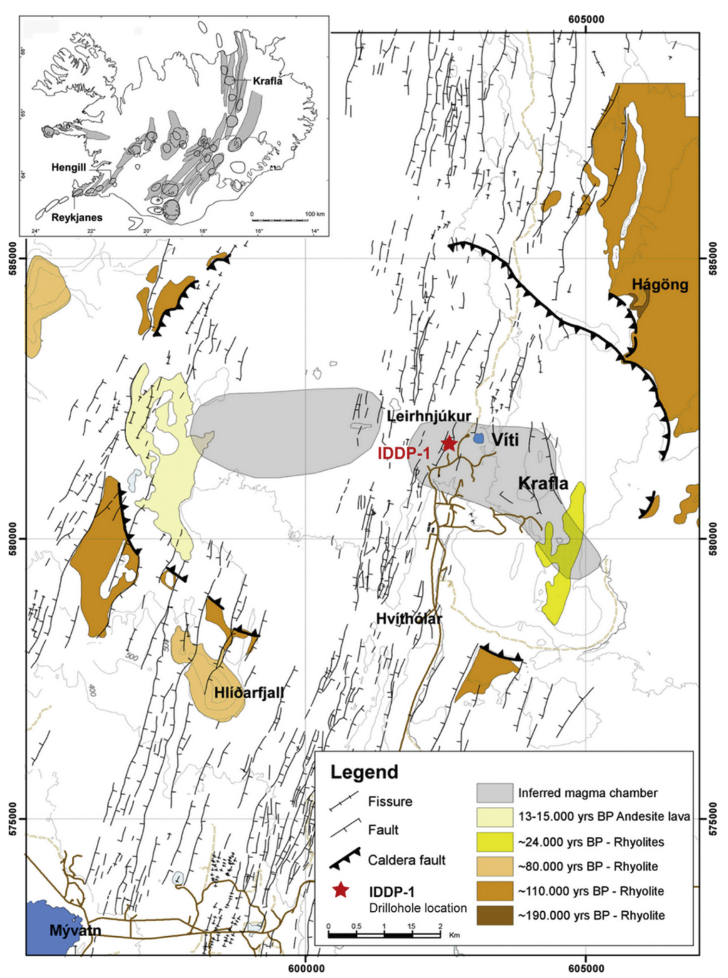
\includegraphics[width=1\linewidth]{img/chapter1/Krafla_1.png}
    \caption{\cite{masotta2018}}
    \label{fig:krafla_map}
\end{figure}

\subsubsection{Volcanic history}
The main structure in the Krafla systems is its caldera, formed around 110000 years ago, during the Eemian interglacial period after a phreatic, dacitic eruption took place, and was followed by two other silicic or semi-silicic eruptions, on 80 ka ago, forming the edifices of Hlíðarfjall to the Southwest of the caldera, Jörundur to the East-Southeast and Rani to the Northwest (\cite{sæmundsson1991}) This volcanism might have formed a inner caldera, now buried by more recent deposits (\cite{arnason2020}). Subglacial eruptions produced characteristic hyaloclastite ridges aligned with the fissure swarm trend within the caldera. Notable examples include the Mt. Krafla itself, which may represent a resurgent dome formed after the caldera collapse (\cite{castillo2021}). 24 ka ago a subglacial fissure eruption formed the obsidian ridge in the Southeastern are of the caldera known as Hrafntinnuhryggur. Alternating with these eruptions, the volcanic activity is dominated by basaltic fissure eruptions an dyke injections.

In the post-glacial era, about 8 ka ago, the spreading shifted from the East to the West of the fissure swarm, although volcanic activity didn't increase during this period. Just one noticeable phreatic eruption took place, at about 5 ka years ago, forming the Hvannstóð crater, in the Northwestern part of the main caldera. 3 ka years ago, the spreading moved back to the East, and since then, eruptions have occur every 300-1000 years (\cite{sæmundsson1991}). During both of these periods the volcanic activity was concentrated, with very few exceptions, on the eastern side fissure swarm due to a 18° difference on the opening directions of the East-side crust of the swarm, between the southern part from the caldera (with an approximate direction of 22°SE) and the northern part (with a direction of 4°SE approximately), according to (\cite{drouin2017}). This may have led to a N-S opening component, favoring magma ascent of magma (\cite{arnason2020}).

The last two eruptive episodes have occurred during historical times: the Mývatn Fires (1724-1729) and the Krafla Fires (1975-1984).

\subsubsection{Mývatn Fires (1724-1729)}
The Mývatn Fires started when a phreatomagmatic eruption occurred inside the caldera, forming the characteristic Víti crater on the 17th of May, 1724 (see the exact location of the crate in figure \ref{fig:krafla_map}. The eruption is believed to have been triggered by the intrusion of rhyolitic magma into the hydrothermal system (\cite{montanaro2021}). The main center of the activity moved towards Leirhnjúkur, situated 2 km West from Víti, with repeated dyke injections into the fissure swarm. In 1727 the peak activity commenced with effusive basaltic fissure eruptions around the area. Two main fissure eruptions occurred between 1727 and 1729 within the caldera, although there is record of a smaller eruption taking place west of Námafjall (\cite{sæmundsson1991}).

\subsubsection{Krafla Fires (1975-1784)}
The Krafla fires is the most recent eruption of the Krafla volcano. This eruptive period is exceptionally significant because it was the first such episode on a mid-ocean ridge segment to be extensively monitored using modern geophysical techniques, providing unprecedented insights into rift dynamics. The episode began in December of 1975 with a small and brief basaltic fissure eruption north of the Leirhnjúkur ridge within the caldera, preceded by an intense earthquake swarm.

It was characterized by repeated episodes of inflation and deflation. The inflation periods, lasting from months to over a year, were interpreted as magma accumulating in a shallow reservoir located approximately 3 km beneath the surface. Seismic studies using S-wave attenuation and P-wave delays supported the presence of a melt-bearing body at depths of 3-7 km (\cite{einarsson1978}). These S-wave "shadows", named as in \cite{arnason2020} can be seen in figure \ref{fig:krafla_map} as the gray-colored shapes referred as inferred magma chamber on the map's legend. The maximum rate of magma inflow into this reservoir during inflation was estimated at 5 m³/s. The rapid deflation events, typically lasting from a day to several months 31, corresponded to the failure of the magma reservoir walls and the lateral injection of magma as dikes into the NNE-SSW trending fissure swarm (\cite{einarsson1980}). In total, 9 of these inflation and deflation episodes actually ended up erupting, with the final eruption of the Krafla Fires taking place in September 1984. A detailed study of the ground deformation during and after this eruption (\cite{tryggvason1986}) suggests that deeper magma reservoirs feed shallower ones, at approximately 2.6 km depth, an idea that partially support the previously mentioned S-waves "shadows" as melt-bearing bodies at depths between 3 and 7 km. The average opening across the 70-80 km affected rift segment has been estimated at 4.3-5.4 meters (\cite{hollingsworth2012}). 

Recent detailed petrological analysis of the lavas erupted during the Krafla Fires has revealed a more complex magmatic system than previously assumed based solely on geophysics (\cite{rooyakkers2024}). Evidence indicates the simultaneous tapping of two distinct basaltic magma reservoirs during several eruptions: a primitive magma sourced from the lower crust (~14-19 km depth) and a more evolved tholeiitic magma from the shallower reservoir system (~7-9 km depth, likely encompassing the 3 km seismically-imaged chamber). Mixing between these two magma types occurred near the northern caldera margin. This implies rapid magma ascent pathways from the lower crust that potentially bypassed the main shallow storage zone, suggesting a decoupling of flow paths and hydraulic connection between reservoirs at different crustal levels during the rifting process and simultaneous feeding of the eruptions in several events.

\subsubsection{Geothermal System}
As previously mentioned, Krafla hosts a high-enthalpy geothermal system located in the center the outer caldera, which provides a geothermal power plant with a production capability of 60 MW. 
A total of 43 wells have been drilled inside the caldera for exploration and production purposes. Some of the wells have also being used for reinjection. Analizeing the well formation temperature from the drilling logs, \cite{mortesen2015}, \cite{arnason2020}, \cite{scott2022} and reference therein suggest the presence of five distinct subfields withing the caldera: Leirbotnar-Vítismór and Suðurhlíðar located west and east of the Hveragil fissure; Hvíthólar on the southern rim of the caldera and Vestursvæði and Sandabotnaskarð, located to the north and south of Suðurhlíðar respectively. 
Leirbotnar-Vítismór subfield is characterized by the presence of an isothermal layer between 500 and 1000 m b.s.l. at 200°C, interpreted as a low permeability aquitard (Bodvarsson, Pruess, et al., 1984; Stefánsson, 1981). This aquitard separates separates the sub-boiling upper reservoir from the underlying two phase zone, which follows the boiling curve with depth.


\subsubsection{Current status}
At present times and moment of production of this thesis, the Krafla volcano is generally considered to be in a state of quiescence following the end of the Krafla Fires in 1984, although ongoing processes related to post-rifting adjustment and geothermal activity continue. 

\subsection{Icelandic Deep Drilling Project - 1}

%============================= SECTIONS =================================

 % uncomment if you want part I
\chapter{Methods}
%--------------------------------------------------
% GOVERNING EQUATIONS
%--------------------------------------------------
In this chapter we present the physical and mathematical model. The governing equations for this problem are the weakly compressible Stokes flow equations for modeling the viscous flow and the heat transfer equation for computing the time dependent thermal evolution of the system.%Explain a bit each of the subsections


\section{Governing equations}
\subsection{Flow equations}
 Stokes flow, also known as creeping flow, describes the motion of viscous, incompressible fluids at very low Reynolds numbers, where inertial forces are negligible compared to viscous forces. Under this regime, the flow is governed by a simplified form of the Navier–Stokes equations, where the inertial terms are omitted. The governing equations consist of the and the conservation of mass, which reduces to the incompressibility condition, and the conservation of momentum, expressed as a balance between the pressure gradient and the viscous forces.
 This is vastly assumed to be a proper approximation for solving magmatic flows that imply large time scales, as mantle and magma chamber convection (include citations here). Whereas the Navier-Stokes equations are used to describe short-term phenomena, such as conduit flow or eruptive processes, the steady Stokes flow is a necessary assumption for us, since it's numerical requirements are considerably lower due to the time-scale of the processes we simulate. The equations are expressed as follows:

 \begin{align}
\nabla \cdot (\rho \mathbf{v}) &= 0 \quad \text{in } \Omega, \\
\nabla \cdot (p\boldsymbol{I} - \tau) &= \rho g\quad \text{in } \Omega,
\end{align}

where $p$ is pressure, $\rho$ is density, $v$ is the velocity vector, $g$ is the gravity vector, $\delta_{ij}$  is identity tensor and $\tau$ is stress tensor which depends on viscosity and strain rate:

\begin{equation}
\boldsymbol{\tau} = \mu \left( \nabla \mathbf{v} + (\nabla \mathbf{v})^\top \right) - \frac{2}{3} \mu (\nabla \cdot \mathbf{v}) \mathbf{I}
\end{equation}

For which $\mu$ is the viscosity of the mixture.
As our model accountes for phase changes within the magma system, such as crystallization and gas exsolution, we need to also account for the density changes. Thus, we include an isothermal compressibility coefficient transforming our incompressible Stokes system into a weakly compressible one. This coefficient is expressed as:

\begin{equation}
\beta_T = \frac{1}{\rho}\bigg(\frac{\delta\rho}{\delta p}\bigg)_T
\end{equation}

The set of conservation equations assumes that the different phases we can find in the magma (melt, crystals and gaseous phases) are mechanically coupled, they have the same velocity. This is justified in the frame of high viscosity magmas and time scales of the order of years, and not larger. 
Our system of equations can also be written and solved in a fully coupled monolithic way as a single transport system (Hauke and Hughes, 1998; Longo et al., 2012b; Garg et al., 2018a):
\begin{equation}
\boldsymbol{F^{a}_{i,i}} = \boldsymbol{F^{d}_{i,i}} + \boldsymbol{S}
\end{equation}


where $\boldsymbol{F_{i,i}^{a}}$, $\boldsymbol{F_{i,i}^{d}}$, and $\boldsymbol{S}$ are the advection flux, diffusion flux and source vectors, respectively, and are defined as:

\begin{equation}
\boldsymbol{F^{a}_{i}} = 
\begin{bmatrix}
\rho v_i\\
p\delta_{ij} 
\end{bmatrix}, ~~~~~~~~~~~
\boldsymbol{F^{d}_{i}} = 
\begin{bmatrix}
0\\
\mathbf{\tau}_{ji}
\end{bmatrix}, ~~~~~~~~~~~
\boldsymbol{S} =
\begin{bmatrix}
0\\
\rho g_i
\end{bmatrix}
\end{equation}

Equation (1) can then be re-expressed for any set of independent variables $\boldsymbol{Y} = [p,\mathbf{v}]$ as follows:


\begin{equation}
    \boldsymbol{A_iY_{,i}} = (\boldsymbol{K_{ij}Y_{,j})_{,i} + S}
\end{equation}


In this equation, $\boldsymbol{A_i = F^{a}_{i,Y}}$ is the $i^{th}$ Euler Jacobian matrix and $\boldsymbol{K = [K_{ij}]}$ is the diffusivity matrix with $\boldsymbol{K_{ij}Y_{,j} = F^{d}_{i}}$.

\subsection{Heat transfer}
In our magma simulations, heat transfer is simulated both inside and outside of the magma domain, although with different approaches. First we solve the heat convection inside the magma domain, as velocity is expected to play an important role on the transport of heat. Then, we couple the boundary of the magma domain with the host rock, trough which the heat will be transferred.

\subsubsection{Magma domain}
Although the fluid motion equations are solved in a fully coupled way as it has been just mentioned, the heat transfer equation needs to be time dependent or transient, since, as opposed to the Stokes assumption, temperature evolves largely with time, as the main process that we are simulating, and the mechanism that controls the evolution of the magma chamber is cooling. The heat transfer equation solved includes advection and diffusion terms, and can be written as follows:

\begin{equation}
\rho c_p \left(\underbrace{\frac{\partial T}{\partial t}}_{\text{Transient term}} + \underbrace{\mathbf{v} \cdot \nabla T }_{\text{Convection term}}\right) = \underbrace{\nabla \cdot (k \nabla T)}_{\text{Conduction term}} + \underbrace{\mathbf{S}}_{\text{Source term}}
\end{equation}

% \begin{equation}
% \rho c_p \left( \frac{\partial T}{\partial t} + \mathbf{v} \cdot \nabla T \right) = \nabla \cdot (k \nabla T) + \sum_{i}^{n} \rho_i qL_i \frac{\partial \phi_i}{\partial t}
% \end{equation}

where $c_p$ is the specific heat capacity, $T$ is the temperature, $\kappa$ is the thermal conductivity and $S$ is any source of sink of heat. Thermodynamical properties of the fluids can be set as fixed or, as they are computed for magma simulations, they can be set as a function of pressure, temperature and composition of the phases. This will be further explained in section XX.

\subsubsection{Rock domain}
The heat transferred across the chamber walls into the host rock is computed by calculating the heat flux along the boundary nodes:

\begin{equation}
\mathbf{q} = -\kappa_m \nabla T_m
\end{equation}

where $\kappa_m$ and $T_m$ the thermal conductivity and the temperature of the magma respectively. Then, the host rock utilizes the heat flux boundary condition to calculate the heat conduction trough the whole domain:

\begin{equation}
\rho_r c_{p_r} \frac{\partial T_r}{\partial t} = \nabla \cdot \left( \kappa_r \nabla T_r \right)
\end{equation}

where $\rho_r$ is the rock density, $c_{p_r}$ is the rock specific heat capacity, $T_r$ is the rock temperature and $\kappa_r$ is the rock thermal conductivity.

Once the new temperature profile is computed along the rocks, the new boundary temperature is passed back to the magma, for utilizing in the next time step.

\subsection{Numerical scheme}
Solution is obtained within a single time step by individually iterating over the three sets of equations as described in the following steps:

\begin{enumerate}
    \item Solve the mass and momentum conservation equations. Solution is then passed to the magma heat transfer equation.
    \item Solve the fluid heat transfer equation for the given time step $t_n$ with the velocity solution obtained from the previous step in the form of weak coupling (meaning that we do not correct the Stokes solution after computing the temperature of the system).
    \item Compute the heat flux on the boundary nodes and pass it to the host rock.
    \item From the heat flux obtained from the magma, compute the new temperature distribution inside the host rock and return the boundary temperature to the magma domain to be used on the following time step.
    \item Print the complete solution for the currently solved time step.
\end{enumerate}

The following chart better exemplifies the logic followed within a time step:

\hspace*{-2cm}
\begin{tikzpicture}[node distance=2cm]
    %\node (start) [startstop] {Start};
    \node (step1) [process, xshift=-2cm] {Solve Stokes equations (mass and momentum)};
    \node (decision1) [decision, right of=step1, xshift=2.90cm] {Solution found?};
    \node (step2) [process, right of=decision1, xshift=2.9cm] {Solve temperature equation};
    \node (decision2) [decision, below of=step2, yshift=-1.5cm] {Solution found?};
    \node (step3) [process, left of=decision2, xshift=-2.9cm] {Heat flux from magma to host rock};
    \node (step4) [process, left of=step3, xshift=-3cm] {Solve heat conduction in the rock};
    \node (decision3) [decision, below, below of=step4, yshift=-1.5cm] {Solution found?};
    \node (step5) [process, right of=decision3, xshift=2.9cm] {Set temperature at the interface for next time step};
    \node (stop) [startstop, right of=step5, xshift=2.9cm] {Assemble and print solution for current time step};
        
    \draw [arrow] (step1) -- (decision1);
    \draw [arrow] (decision1) -- (step2) node[midway, above] {Yes};
    \draw [arrow] (decision1.north) to[bend left=-45] node[midway, above] {No} (step1.north);
    \draw [arrow] (step2) -- (decision2);
    \draw [arrow] (decision2) -- (step3) node[midway, above] {Yes};
    \draw [arrow] (decision2.east) to[bend left=-45] node[midway, right] {No} (step2.east);
    \draw [arrow] (step3) -- (step4);
    \draw [arrow] (step4) -- (decision3);
    \draw [arrow] (decision3) -- (step5) node[midway, above] {Yes};
    \draw [arrow] (decision3.west) to[bend left=45] node[midway, left] {No} (step4.west);
    \draw [arrow] (step5) -- (stop);
    % \draw[dashed, red] (current bounding box.south west) rectangle (current bounding box.north east);
\end{tikzpicture}


%--------------------------------------------------
% BENCHMARKS
%--------------------------------------------------
\section{Benchmarking examples}
A number of benchmarking exercises have been made in order to test the accuracy and consistency of the new solver. We show two benchmark exercises for the non-thermally coupled Stokes flow and other four for the complete, thermally coupled solver: SolCx and SolKz from \cite{durez2011}, 2D convection cases 1c, 2a and 3 from \cite{blankenbach1989benchmark}, and 2D cylindrical shell benchmark from ASPECT (\cite{heister:etal:2017,kronbichler:etal:2012,aspect-doi-v2.5.0,aspectmanual}), described as taken from Davies et al case 1.1 BA-Ra104-Iso-ZS (paper yet to be published).

\subsection{SolCx and SolKz}
This two benchmarks test the accuracy of the stand-alone Stokes equations with varying viscosity. The domain is in both cases a square box ($l/h = 1$) with all boundaries set to be free slip.
In the case of SolCx, fluid flow is driven by a sinusoidal force:
\begin{equation} 
    F = (0,-sin(\pi y)cos(\pi x))
\end{equation}
and a sharp viscosity jump set as follows:
\begin{equation}
\eta (x) =
\begin{cases} 
1, & \text{if } 0 \leq x \leq 0.5 \\
10^6, & \text{if } 0.5 < 0 \leq 1 Ma
\end{cases}
\end{equation}
For the SolKz case, the driving force should be expressed as:
\begin{equation} 
    F = (0,-sin(2y)cos(3\pi x))
\end{equation}
while the viscosity distribution is defined as:
\begin{equation}
    \eta(y)=exp(2By)
\end{equation}
Results for both benchmarks are depicted in figure 1, matching perfectly the benchmark results described in the reference paper, hence assessing the Stokes solver accuracy.
\begin{figure}
    \centering
    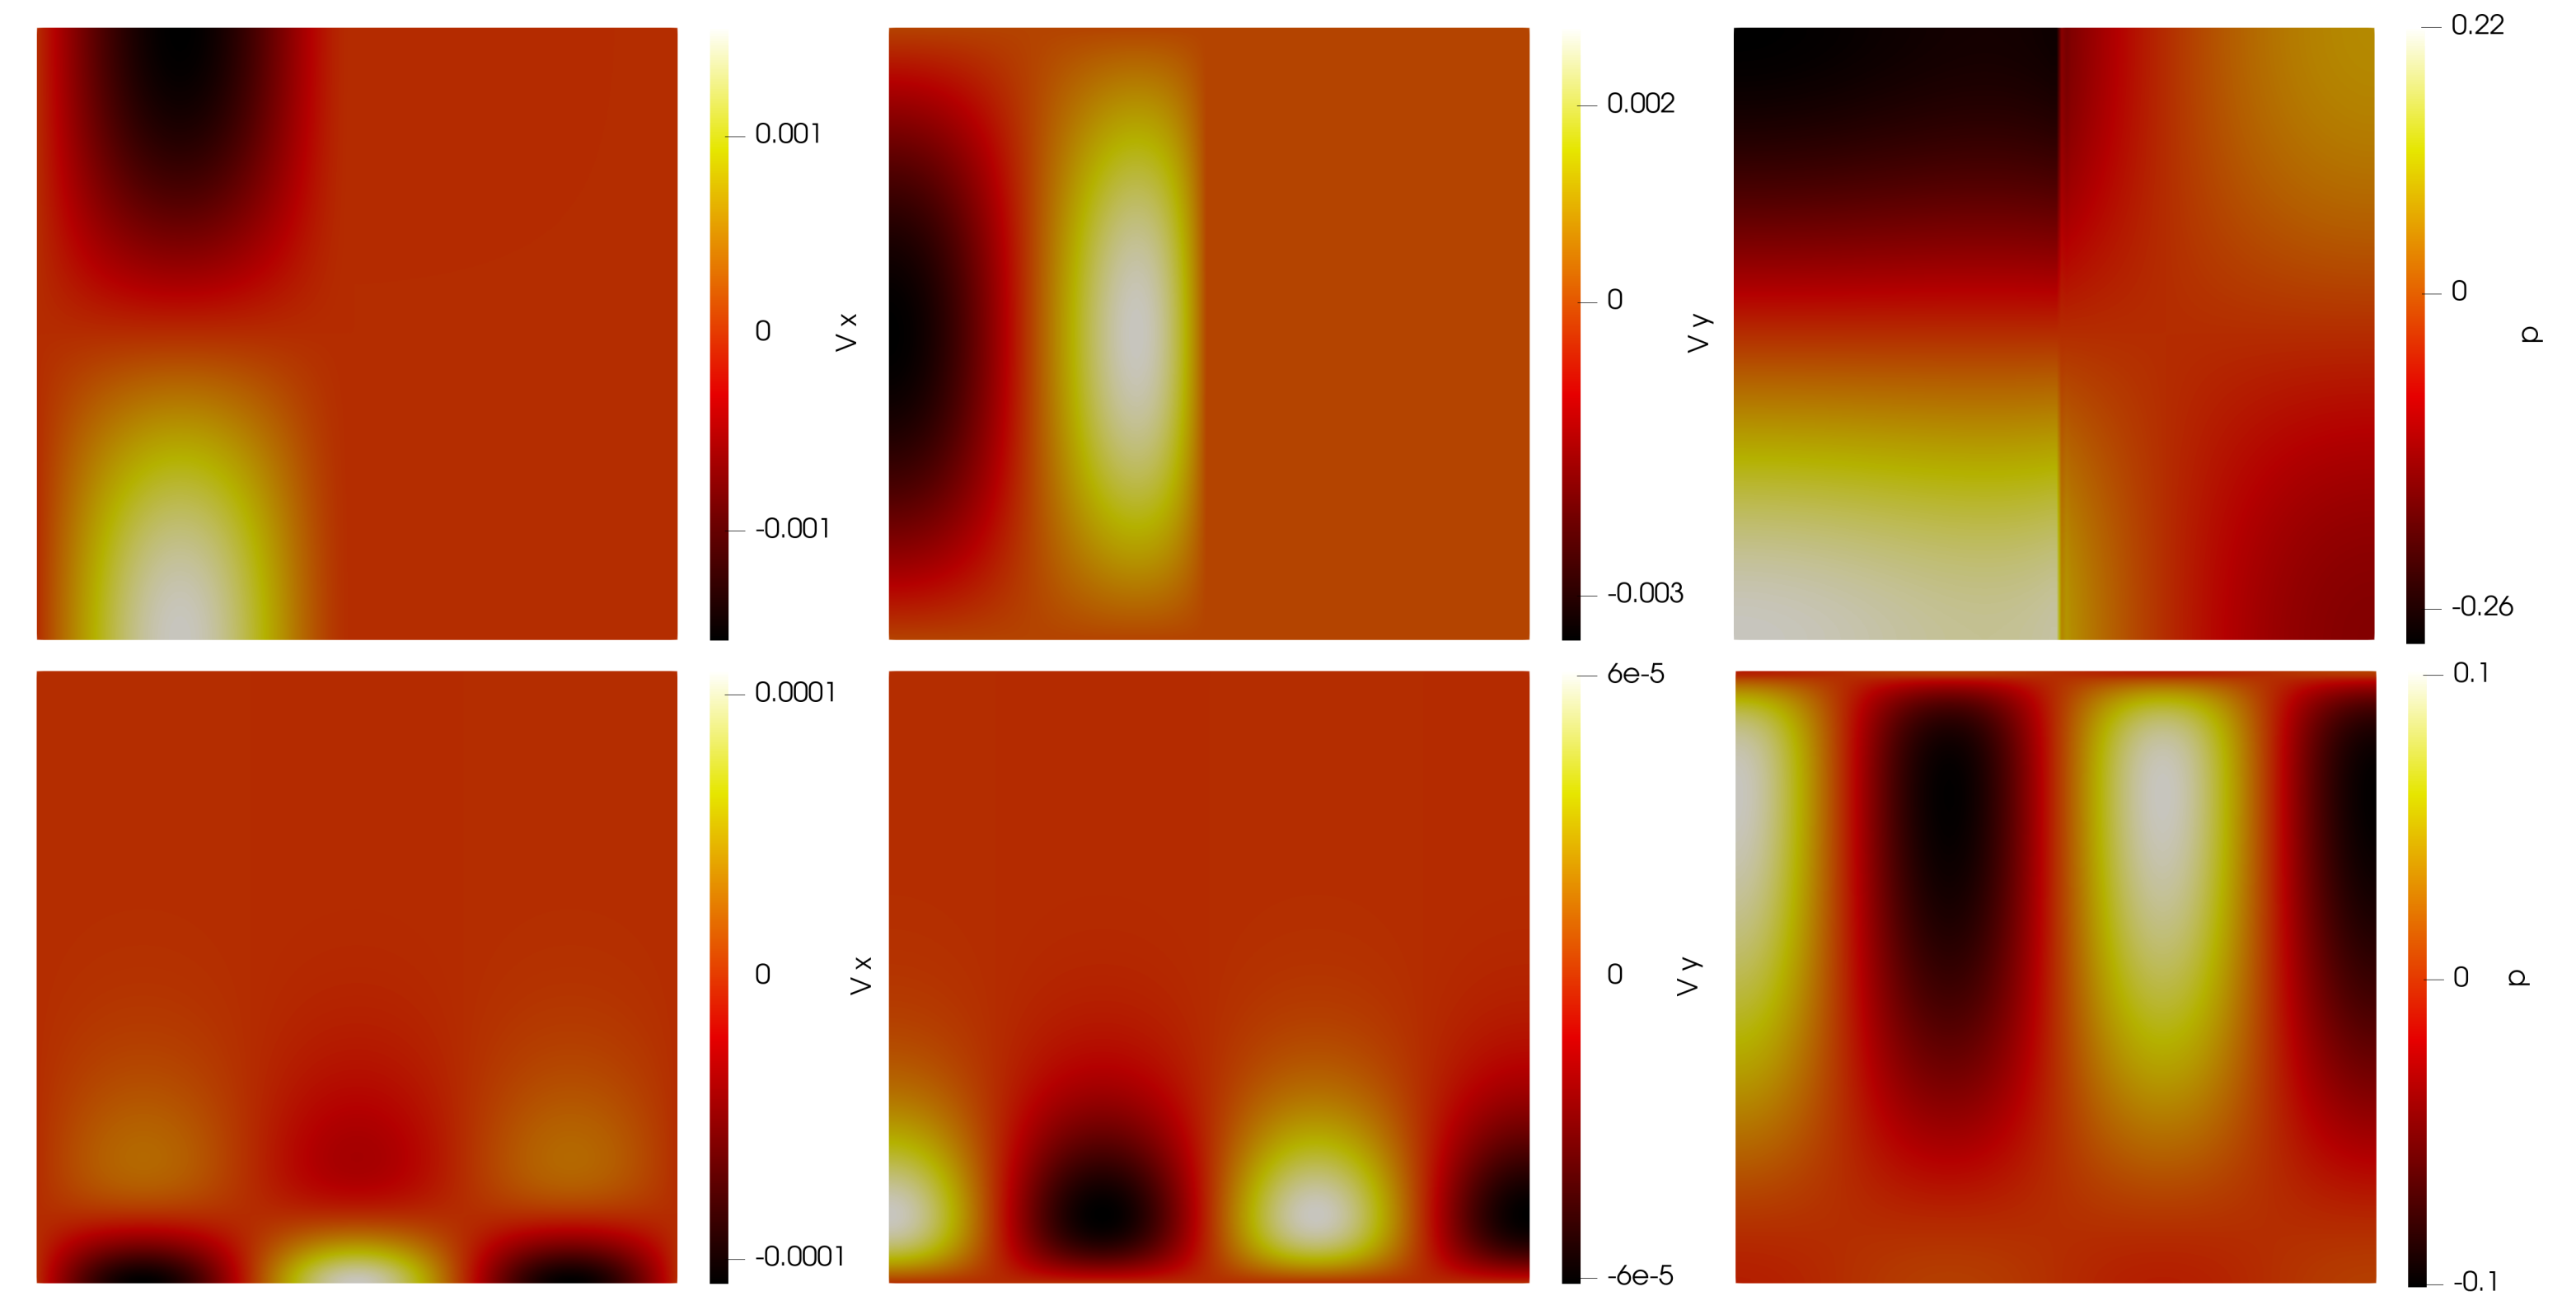
\includegraphics[width=1\linewidth]{img/chapter2/benchmarks/sols.png}
    \put(-442,100){SolKz}
    \put(-442,200){SolCx}
    \caption{Horizontal and vertical velocity fields as well as and pressure distribution for SolCx benchmark on top, and SolKz benchmark on the bottom of the figure}
    \label{fig:enter-label}
\end{figure}

\subsection{2D convection 1c}
This benchmark is described as steady convection with constant properties, including constant viscosity. Domain is a square box ($l/h = 1$) and the temperature is fixed to zero on top and to $\Delta T$ on bottom. There are no internal heat sources. No normal-velocity flux on the side boundaries (reflective symmetry conditions) and free slip condition (zero shear stress) on all boundaries. The Rayleigh number is
\begin{equation}
   Ra = \frac{\alpha g \delta T h^3}{\kappa \mu}
\end{equation}
and for this case it is set to have a value of $10^6$.
This benchmark requires calculating the Nusselt number as in:

\begin{equation}
   Nu = -\frac{\int_{0}^{1}\delta_zT(x,z=h)dx}{\int_{0}^{1}T(x,z=0)dx}
\end{equation}
the root-mean-square (rms) velocity:

\begin{equation}
   v_{rms} = \frac{h}{\kappa} \bigg[\frac{1}{hl}\int_{0}^{l}\int_{0}^{h}(u^2+w^2)dzdx\bigg]^{\frac{1}{2}}
\end{equation}

and the temperature gradients at the corners:

\begin{equation}
    q = \frac{-h}{\Delta T}\bigg(\frac{\delta T}{\delta z}\bigg)
\end{equation}

All of this three quantities are non-dimensional in this examples. Results are within the benchmark limits, with a Nusselt number of 20.73, a v$_{rms}$ of 849.97, q$_1$ equal to 34.5 and q$_2$ equal to 0.863.  
Figure 1 shows the temperature distribution at the steady state of the simulation, showing a right-wise convective pattern.


\subsection{2D convection 2a}
In this case, non dimensional viscosity is temperature and depth dependent following this equations:
\begin{equation}
    \mu = \mu_0 exp\bigg[-\frac{bT}{\Delta T} + \frac{c(1-z)}{h}\bigg]
\end{equation}
with $b = ln(1000)$ and $c = 0$ and $\mu_0$ is 1 in its dimensionless form. Boundary conditions for this case are the same as for the previous one and Rayleigh number has a value of $10^4$. Requirements for this example are the same as for the previous one (case 1c).
The results for this quantities are: Nu equal to 10.29, v$_rms$ equal to 499.74 and q$_1$ and q$_2$ equal to 18.04 and 1.01 respectively. 
Figure 2 shows temperature and temperature contours distributions and velocity and with streamlines once steady state is achieved. 

\subsection{2D convection 3}
This time-dependent case of convection has constant viscosity and internal heating. The domain changes to an aspect ratio of $l/h = 1.5$. Side boundaries again have reflective symmetry conditions. No-slip conditions on top and bottom. Temperature at the top is zero, while at the bottom of the domain, the heat flux is zero.


\subsection{2D cylindrical shell}
This case is described as a 2D non-dimensional spherical earth with an outer radius on 1.22 and an inner radius of 2.22. Temperature is 1 in the internal boundary (inner radius) and 0 in the outer as an initial condition. Boussinesq approximation is assumed, and non-slip boundary conditions. Rayleigh number is $10^4$ and the initial temperature distribution follows a spherical harmonic of degree 0 and order 4.
The simulation should arrive to an steady state stage in which four convective cells have formed, staged that is successfully reached, as seen in figure X.

\begin{figure}
    \centering
    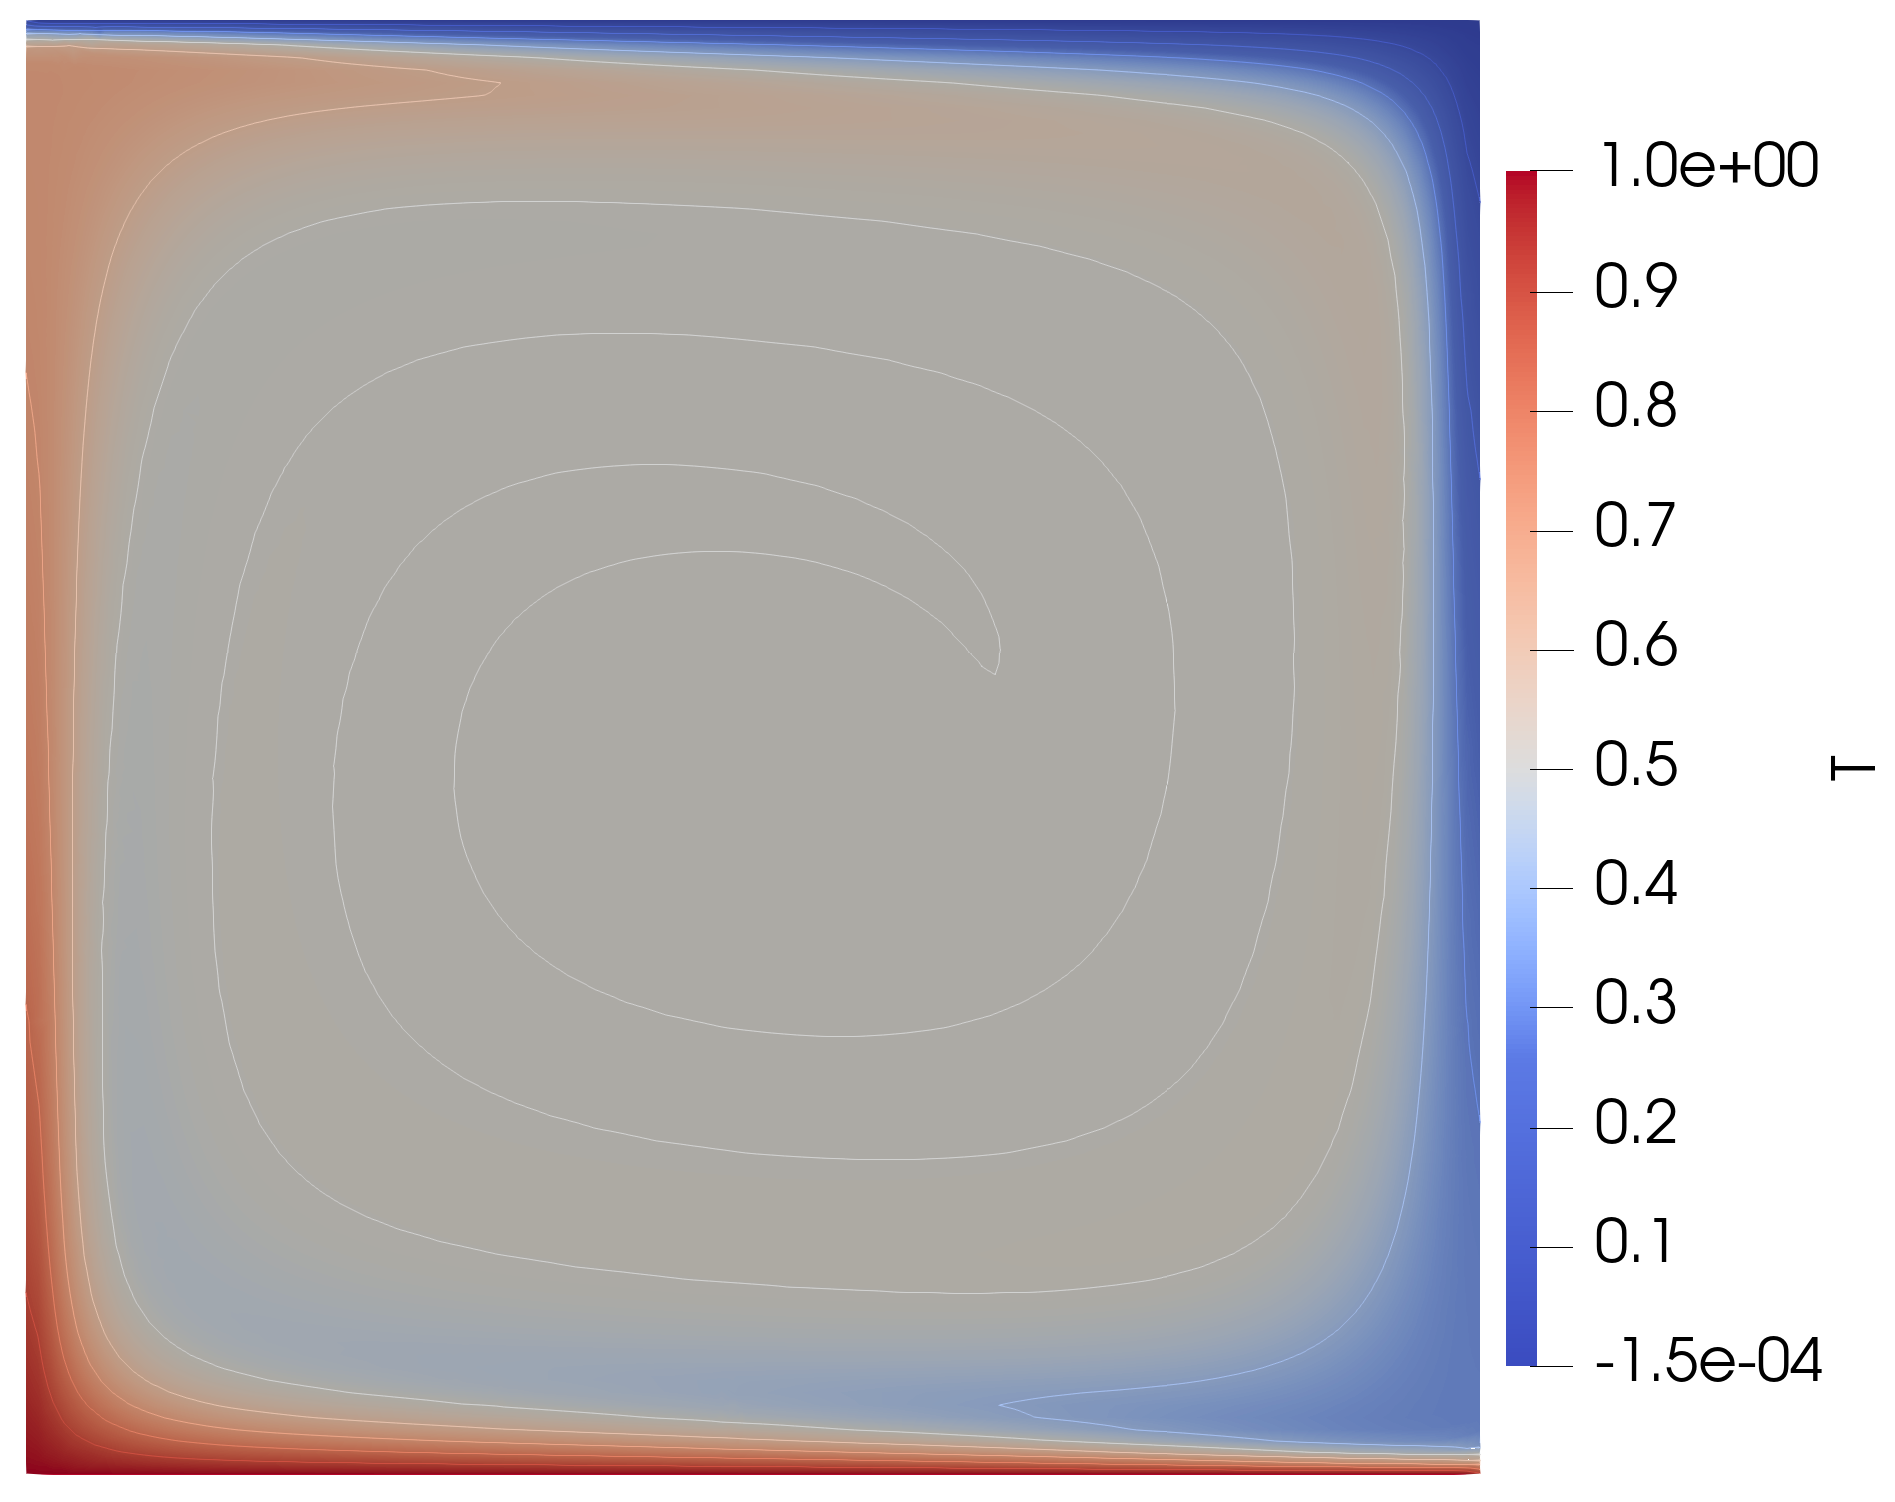
\includegraphics[width=0.75\linewidth]{img/chapter2/benchmarks/contours.png}
    \caption{Temperature field for the 2D convection 1c benchmark once it has reached the final steady state stage}
    \label{fig:enter-label}
\end{figure}


\begin{figure}
    \centering
    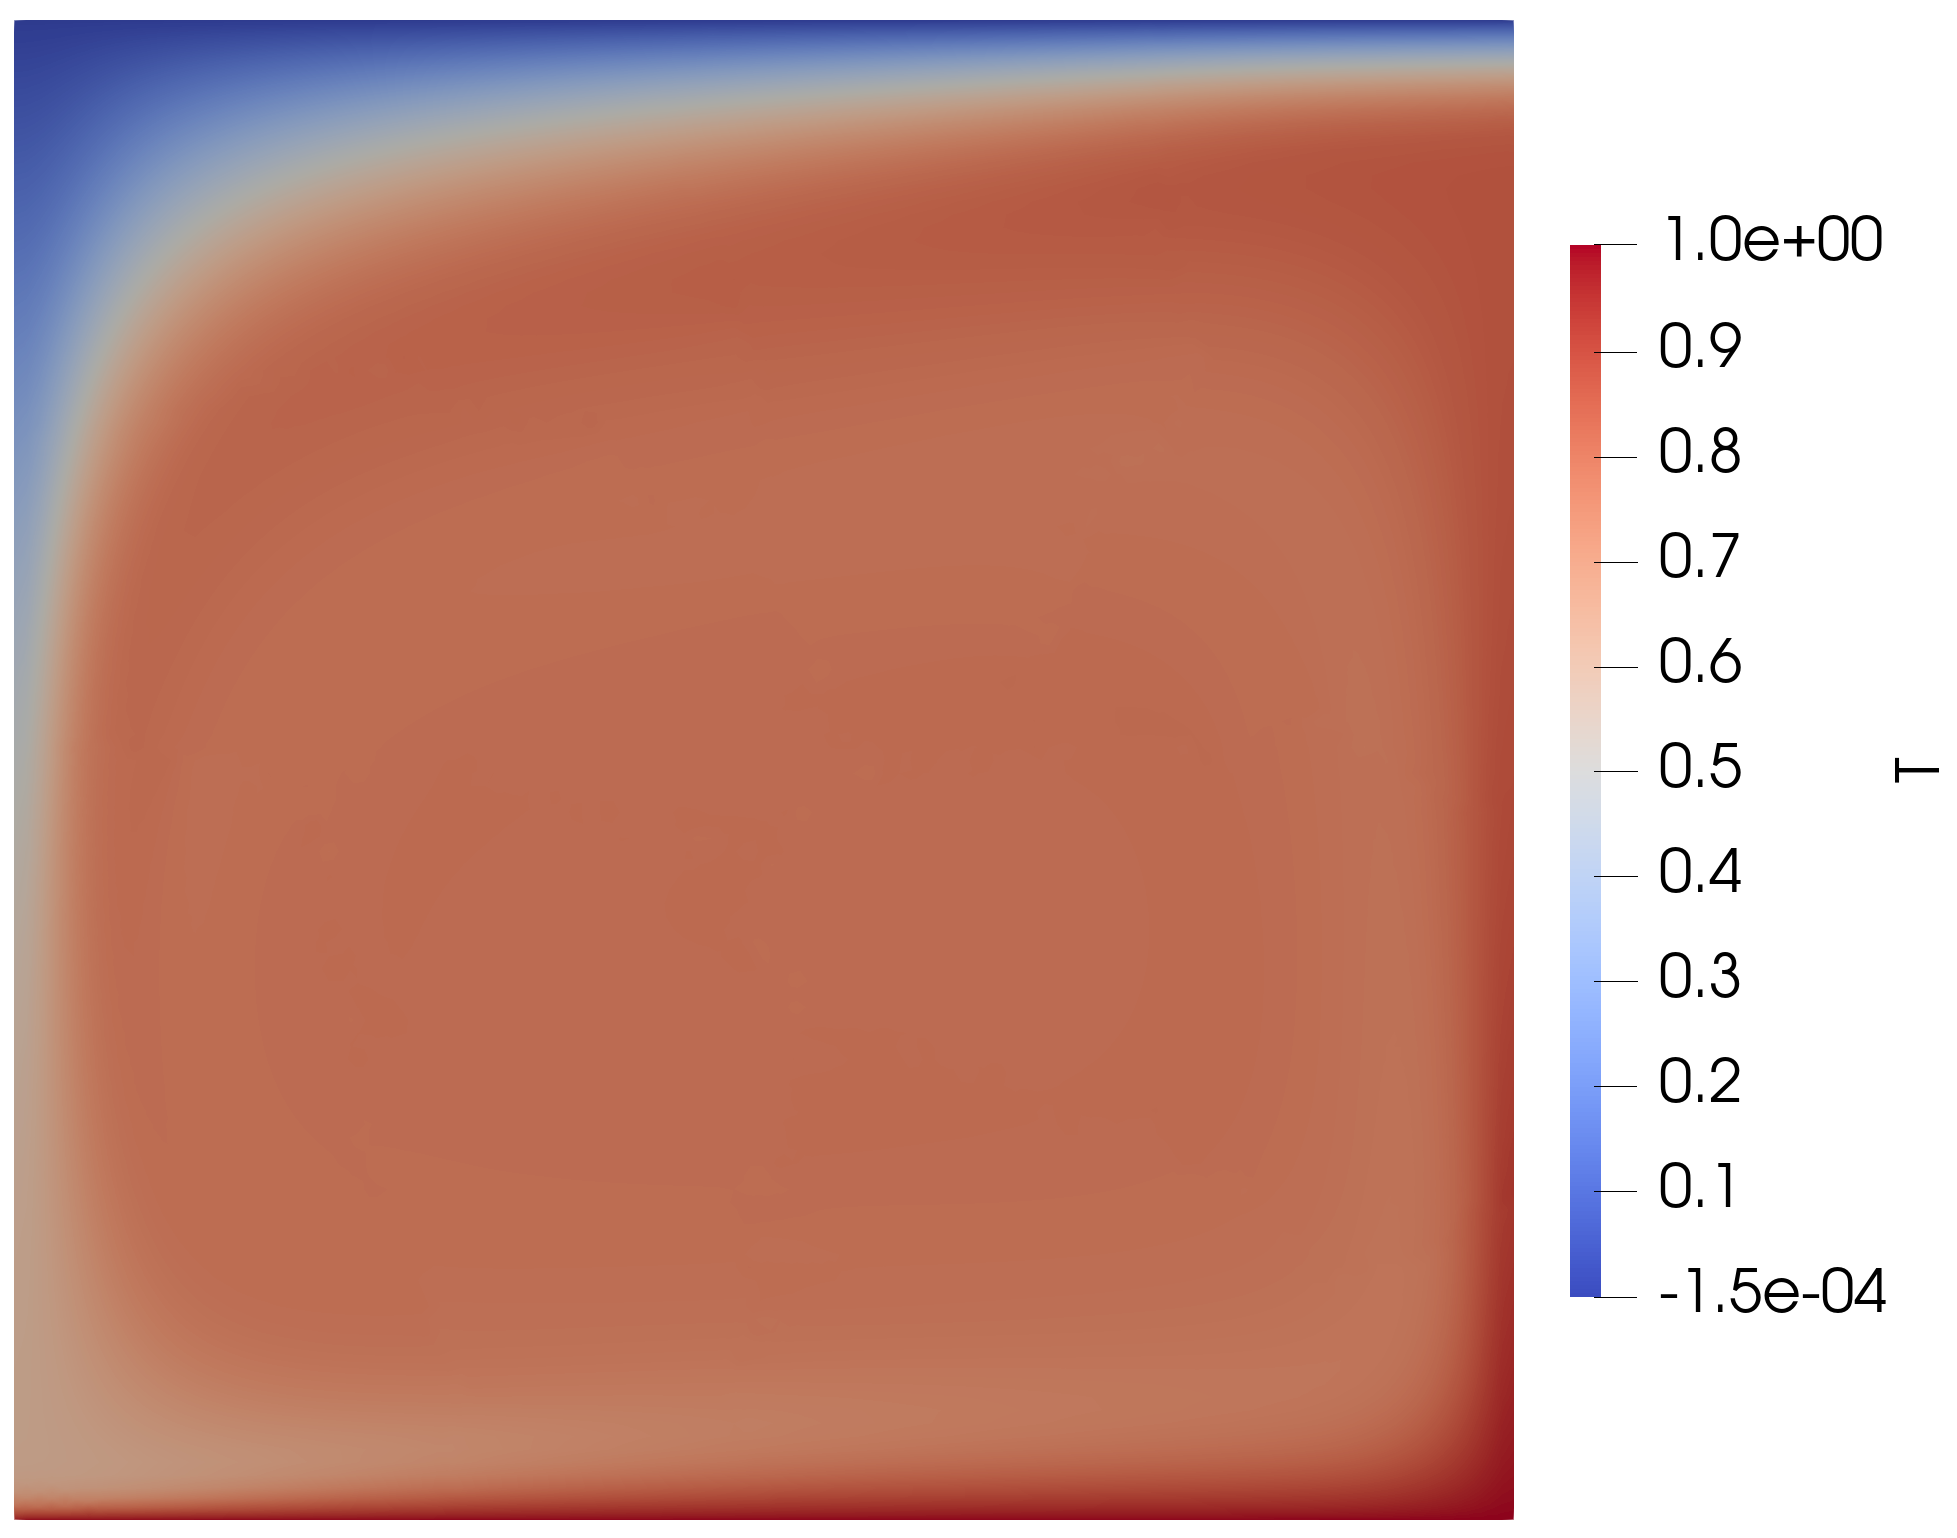
\includegraphics[width=0.75\linewidth]{img/chapter2/benchmarks/temp.png}
    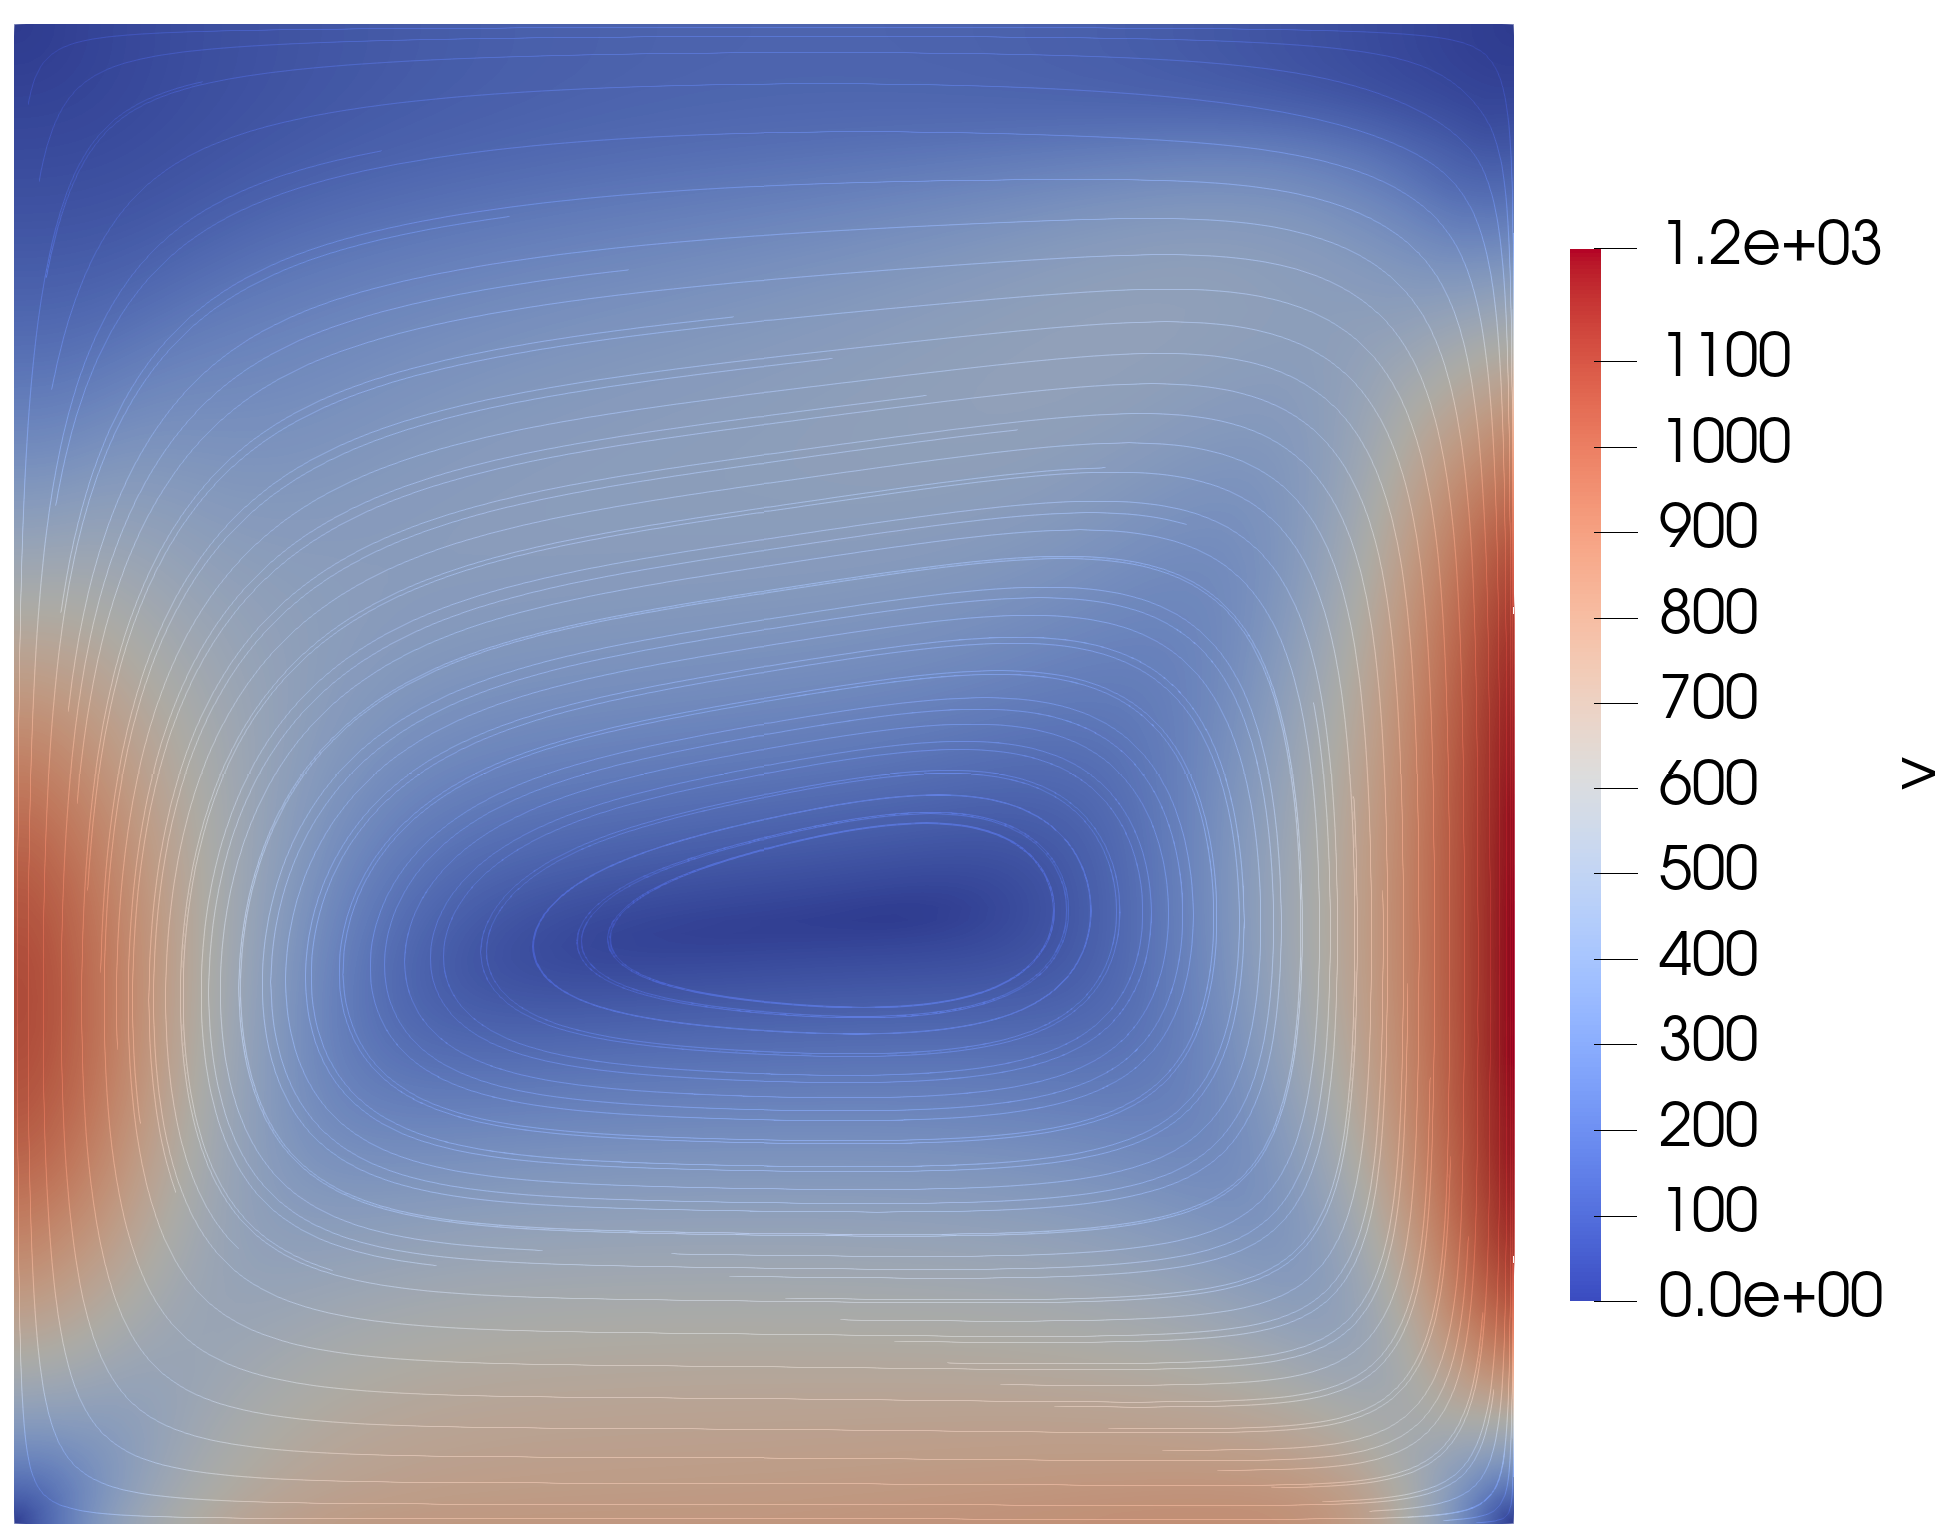
\includegraphics[width=0.75\linewidth]{img/chapter2/benchmarks/streamlines.png}
    \caption{Temperature field for the 2D convection 1c benchmark once it has reached the final steady state stage}
    \label{fig:enter-label}
\end{figure}

\begin{figure}
    \centering
    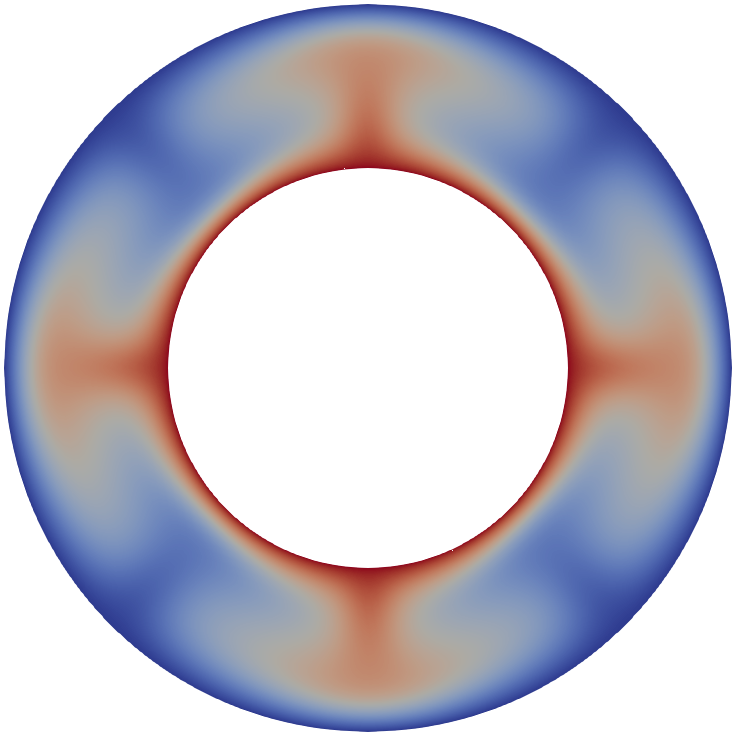
\includegraphics[width=0.75\linewidth]{img/chapter2/benchmarks/t_1.png}
    \caption{Temperature field for the 2D cylindrical benchmark once it has reached the final steady state stage}
    \label{fig:enter-label}
\end{figure}


\subsection{OUR OWN BENCHMARK}
% Develop a simple crystallization and exsolution temperature equations, just normal relationships with T (and P?) 
Due to the significant lack of benchmarking exercises for the thermally coupled stokes flow under magmatic conditions, we propose a benchmark simulation. A simple setup is presented: a rectangular magma chamber 1250 meters long and 500 meters high, with an outer 500 meters rectangle that is set to be the host rock. Initial pressure of the magma is 50 MPa at the top, evolving towards the bottom according to  , while the initial temperature is 900°C. Initial temperature of the surrounding rocks is 350°C. No-slip condition is applied to all boundaries of the magma domain.  
Crystallization and exsolution are defined as simple temperature dependent exponential functions as follows the:

% \begin{equation}    
% \begin{array}{cc}
%     \phi_{cryst}(T) =
%     \begin{cases} 
%     0.1, & T \leq 700 \\
%     0.1* \left(\frac{900 - T}{200} \right)^2, & 700 < T \leq 900 \\
%     0, & T > 900
%     \end{cases}
%     & \ \ \ \ \ \ \
%     \phi_{gas}(T) =
%     \begin{cases} 
%     1.0, & T \leq 700 \\
%     \left(\frac{850 - T}{200} \right)^2, & 700 < T \leq 850 \\
%     0, & T > 850
%     \end{cases}
% \end{array}
% \end{equation}

\begin{equation}   
    \phi_{cryst}(T) =
    \begin{cases} 
    1, & T \leq 700 \\
    0.1* \left(\frac{850 - T}{150} \right)^2, & 700 < T \leq 850 \\
    0, & T > 850
    \end{cases}
\end{equation}

\begin{equation}
    \phi_{gas}(T) =
    \begin{cases} 
    0.1, & T \leq 700 \\
    \left(\frac{900 - T}{200} \right)^2, & 700 < T \leq 900 \\
    0, & T > 900
    \end{cases}
\end{equation}

This functions ensure a fully crystallized and exsolved magma at temperatures bellow 700°C and a fully melted magma at temperatures above 900°C, as can be easily appreciated in figure XX.

\begin{figure}
    \centering
    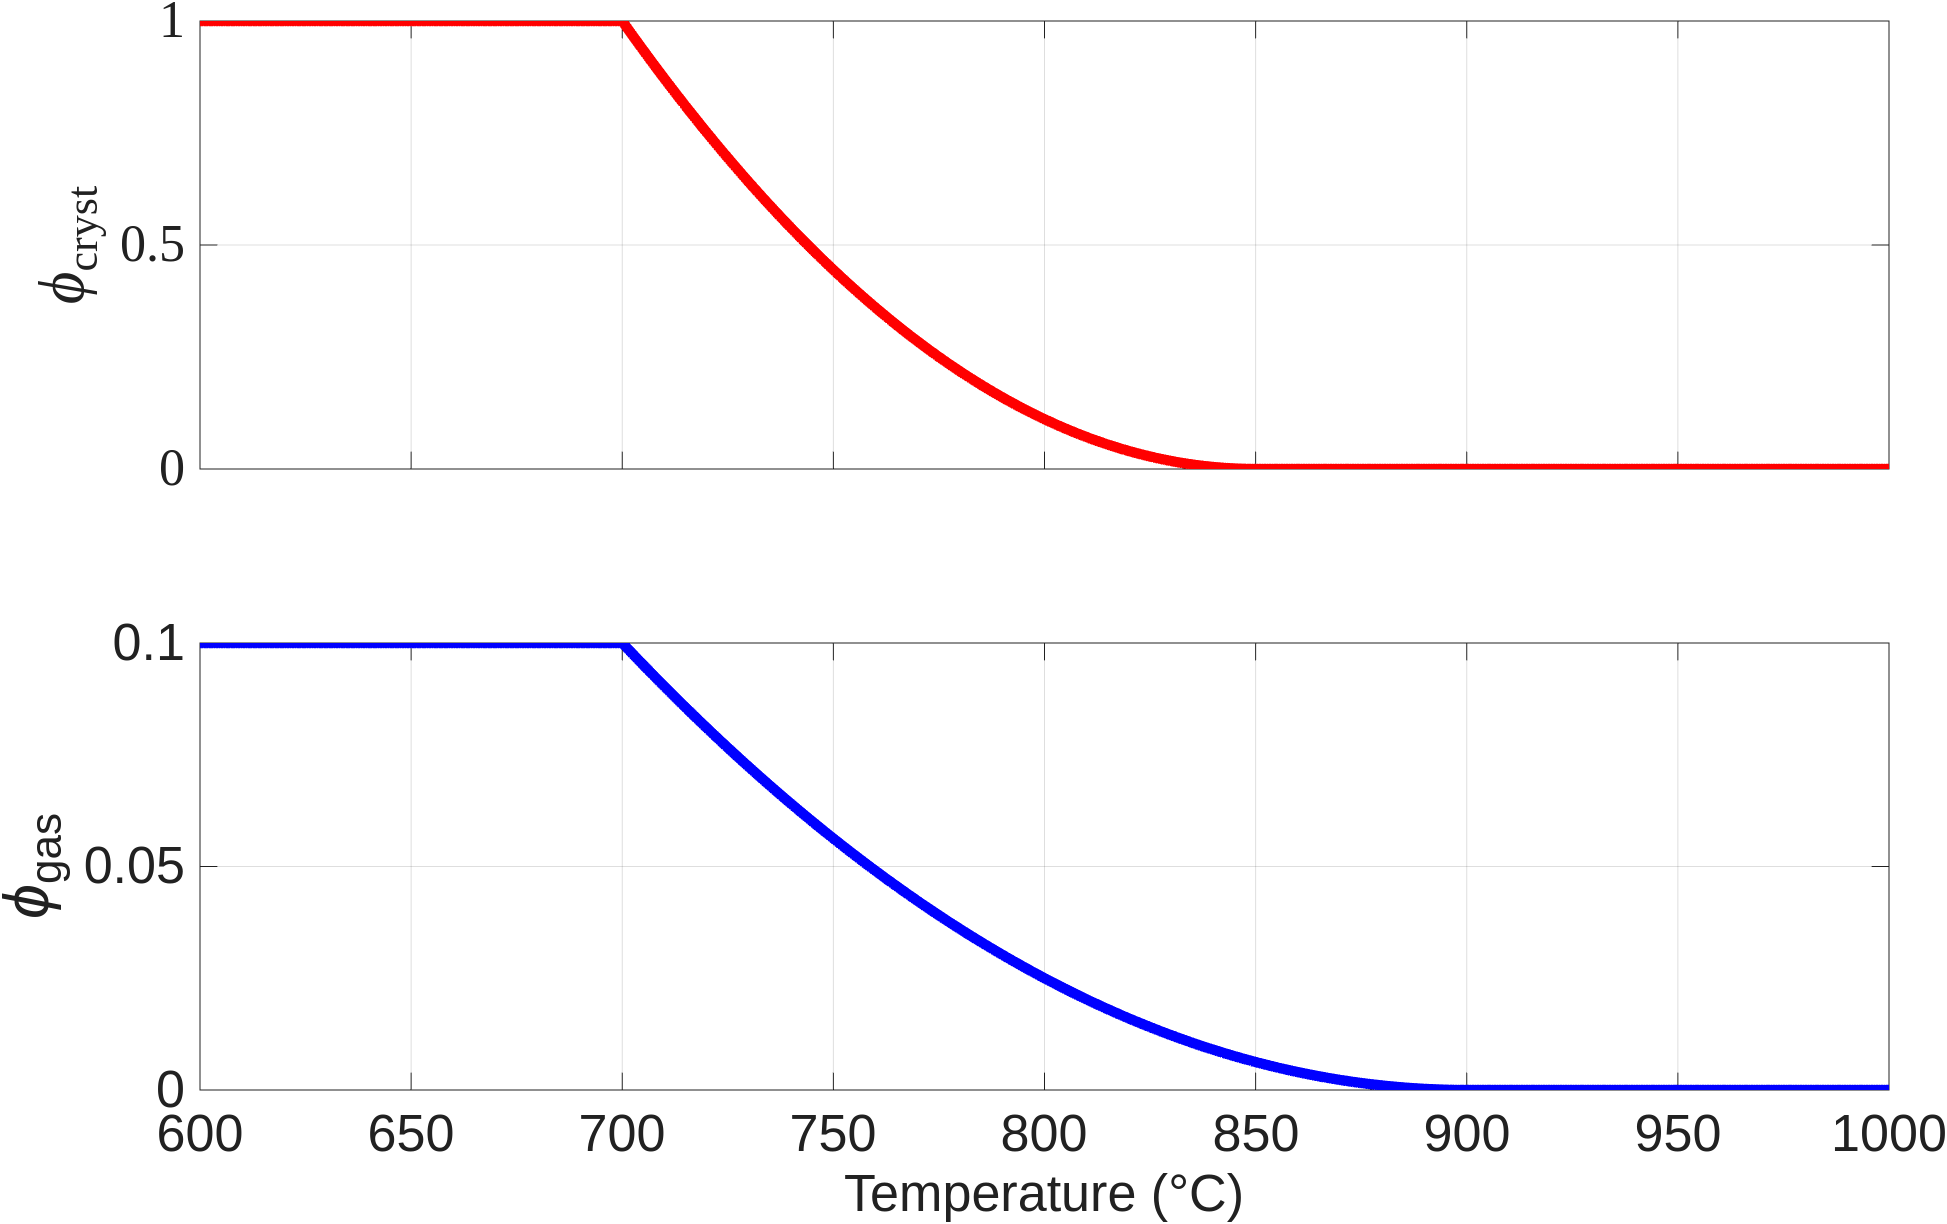
\includegraphics[width=1\linewidth]{img/chapter2/benchmarks/phis.png}
    \caption{Crystal and gas fractions exsolution curves for the proposed benchmark exercise}
    \label{fig:enter-label}
\end{figure}

The properties for each phase are described in the following table:

\begin{table}[H]
\resizebox{\columnwidth}{!}{%
     \begin{tabular}{|c|c|c|c|c|}
     \hline
          & density($g/m^3$) & thermal conductivity($W/mK$) & specific heat capacity($J/kg°C$) & latent heat($J/kg$)\\ 
         \hline
         Melt & 2400 & 1.0 & 1300 & \\
         \hline
         Crystals & 2600 & 3.0 & 1000 & 200000\\
         \hline
         Gas & 200 & 0.1 & 2000 & -100000\\
         \hline
    \end{tabular}
    }
     \caption{Material properties for the different phases present in the magma, for the proposed benchamr simulation}
     \label{tab:enter_label}
 \end{table}


\section{Thermomechanical modeling}
\subsection{Magma properties}
Physical properties are fundamental in the understanding of the behavior and evolution of magmas. They determine the velocity at which magmas move, how fast they cool, how they crystallize and even erupt. For instance, density controls buoyancy and has an strong influence on whether a magma will ascent, stall, or sink, directly influencing magma chamber formation. Heat capacity dictates how much energy a magma is able to store and how resistant it is to temperature variations, affecting the longevity and thermal stability of magma bodies. Thermal conductivity regulates how efficiently magmas lose heat to surrounding rocks, shaping the rate of crystallization and the thermal evolution of intrusive systems. Viscosity controls magma mobility, eruption style, and even the formation of crystal mushes. 

Thus, their importance is of the utmost essence, and need to be properly and realistically modeled in order to maximize the resemblance between the simulated results and reality.  As most of the properties are well constrained by diverse models and natural observations, they serve as the link between the computational domain and the natural world. 

In our simulations, the magmatic properties are computed as a bulk quantities, meaning that the three coexisting phases contribute to the total value of a said property proportionally to its abundance within the magmatic system.
\subsubsection{Temperature}
Temperature constitutes one of the, if not the most important variables controlling magma generation, evolution and overall behavior. It determines whether rocks remain solid, partially or fully molten, and it directly influences fundamental properties such as viscosity, density and crystallinity. Higher temperatures promote low viscosity magmas, magmas capable of flowing and convecting. Cooling drives crystallization, increases viscosity, and eventually leads to solidification. Temperature also controls phase equilibria, determining which minerals crystallize at different stages and influencing the chemical differentiation of magma. Additionally, it affects the solubility of volatiles, the rate of diffusion and the kinetics of chemical reactions. In magma chambers, spatial and temporal variations in temperature can create thermal gradients that drive convection, melt segregation, and even reactivation of previously solidified zones. Overall, temperature is not only a measure of thermal energy but a key control on the dynamics, structure, and eruptive behavior of magmatic systems.

In the present study, temperature is both the solution of the heat transfer equations and an input parameter in computing the phase equilibria and magmatic properties. It is of the upmost importance when analizing results
\subsubsection{Pressure}
Pressure is, alongside temperature, a fundamental variable in any magmatic system with a profound effect on the physical, chemical and phase behavior of magma. It strongly controls gas solubility, favoring volatile dissolution at higher pressures, thereby affecting magma viscosity, crystallization temperatures, and eruptive potential. It is also important on determining melting and crystallization paths. As magma ascends toward the surface, decreasing pressure triggers volatile exsolution, bubble growth, and potentially explosive eruptions if gas escape is restricted. Changes in pressure also shift mineral stability fields, influencing which phases crystallize and when, thus shaping the final rock paragenesis. Furthermore, pressure affects magma chamber dynamics by modulating buoyancy, convection, and the potential for magma recharge or chamber collapse.

Pressure is computed as part of the solution of the Stokes equations alongside the velocity. The initial pressure distribution, however, is computed to be a horizontally uniform profile.

\subsubsection{Volatiles}
Volatiles make up for the one of the three possible phases that are found in magmas, alongside melt and crystals. The most abundant one is water ($H_2O$), followed by carbon dioxide ($CO_2$), and, normally in smaller amounts than the first two, sulfur species ($SO_2$ and $H_2S$) and others. These gases have a profound influence in the physical behavior of magmas, as well as in their chemical evolution, and have major importance regarding eruptive dynamics. Gases in magmas can be found dissolved in the fluid phase when pressure is sufficiently high, and exsolved, forming bubbles in the magma. Dissolved volatiles reduce the viscosity and lower the liquidus of the melt, delaying the formation of crystals and enhancing magma mobility. On the contrary, the role of bubbles can either reduce or increase the viscosity of the magma, as will be discussed further below. Bubble formation normally leads to magma overpressure and, ultimately, volcanic eruptions. Also, the amount and type of volatiles have an deep control on weather an eruption es effusive or explosive.

In this work, the partition between the dissolved and exsolved volatiles is done utilizing the equation of state of SOLWCAD (\cite{papale2006}). SOLWCAD is a numerical software initially written in FORTRAN that computes the fully non-ideal and multi-component compositional-dependent saturation surface of $H_2O$ and $CO_2$ in silicate melts over a wide range of pressure and temperature conditions. The software has been rewritten in C++ and implemented within GALES  to allow run-time gas-equilibria computations for any P-T-X inside the magma domain. 

\begin{figure}
    \centering
    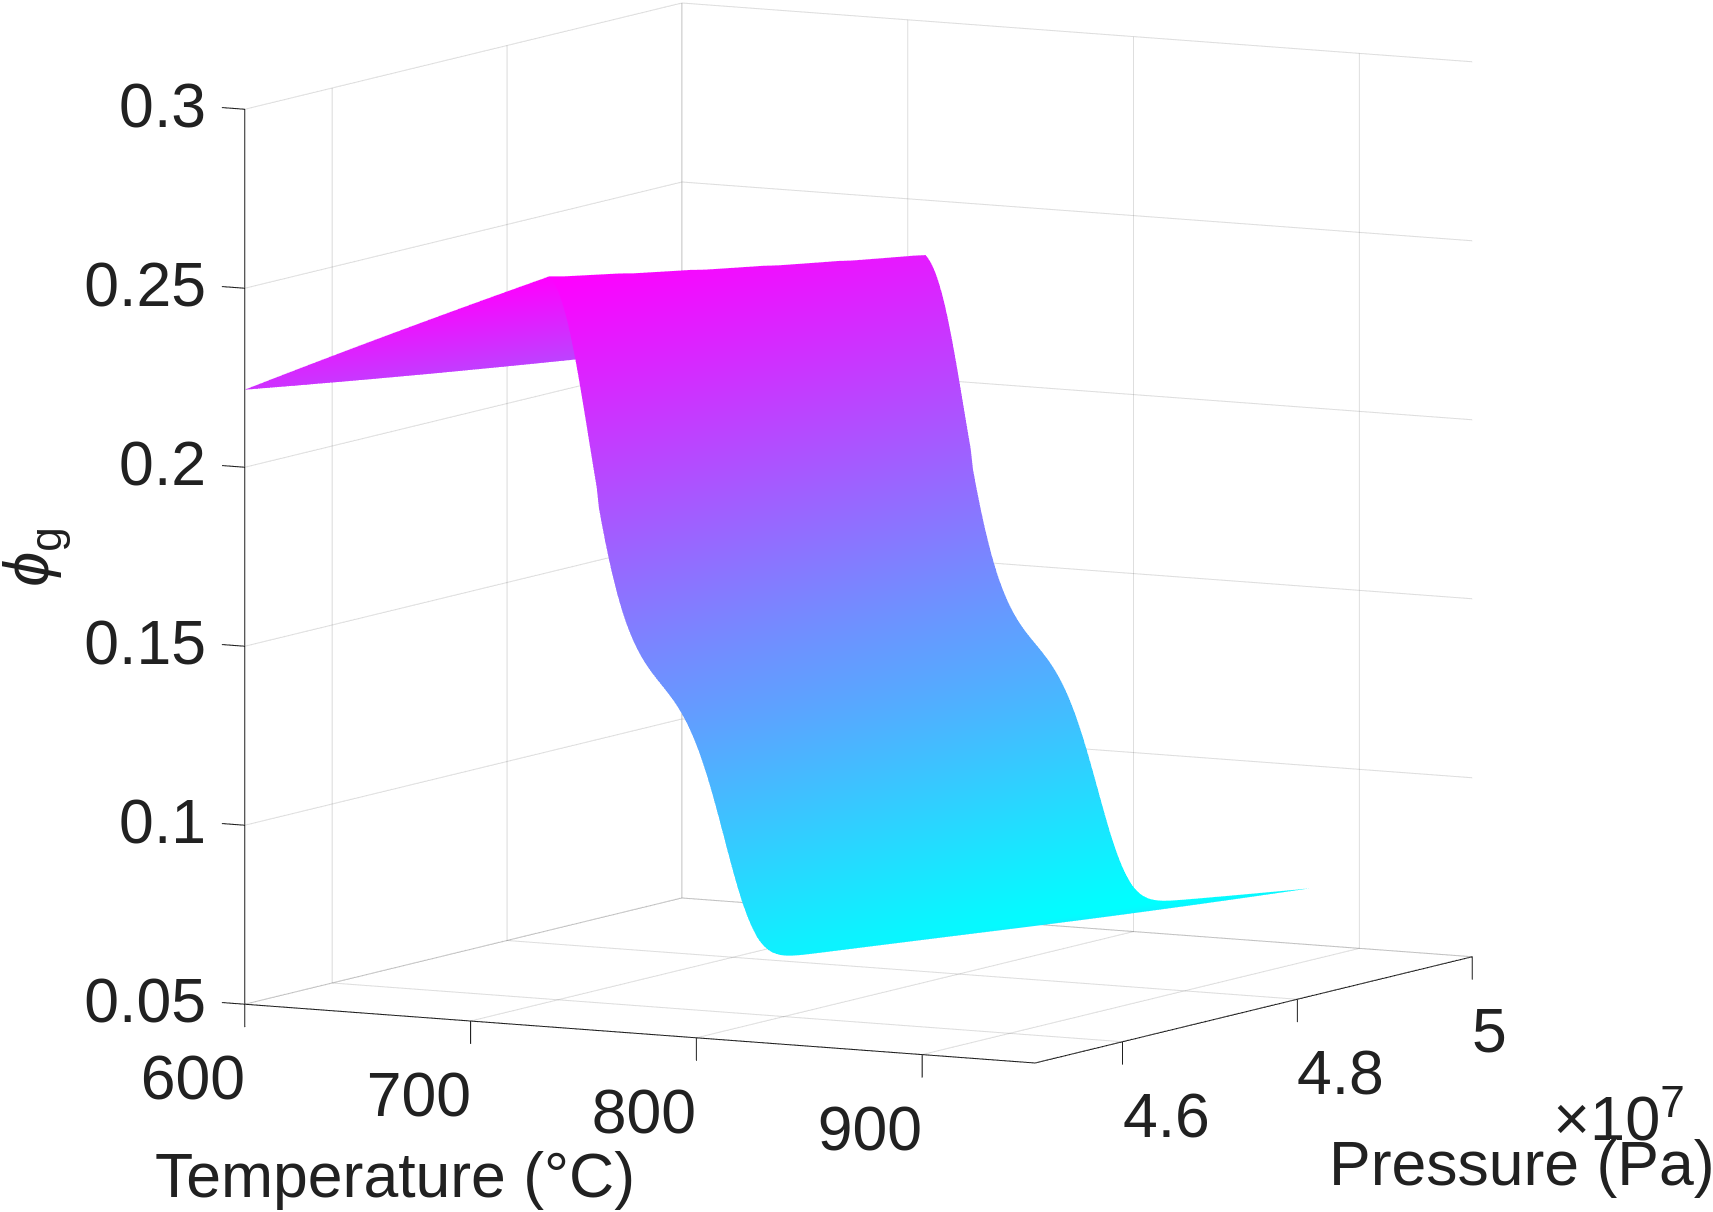
\includegraphics[width=1\linewidth]{img/chapter2/properties/vf_g/vf_g.png}
    \caption{Bulk thermal conductivity modeled for 45 MPa}
    \label{fig:enter-label}
\end{figure}

\subsubsection{Crystallinity}
Crystallinity is crucial in the understanding of magmas evolution, as it serves as an indicator of its thermal, chemical and mechanical state. As magmas cool, they normally undergo partial crystallization, influencing properties such as viscosity, density and thermal conductivity, but not only, since the impact of crystallinity also extents to the magma dynamics and eruptive potential and style. Magmas with low crystal fraction behave as fluids, capable of mixing and flowing, while high-crystallinity ones (typical more than 50\% crystal fraction) typically form rather immobile crystal mushes. Crystallinity plays a fundamental role in magma differentiation, as melt segregation is normally produced due to crystal accumulation, modifying melt and mineral composition, and leading to the generation of evolved magmas.

Crystal fraction can be computed from a number of numerical models, empirical data calculated from petrological observations or simply by setting a fixed a unique value, typical for isothermal simulations. Within GALES, any of these can be easily implemented. For this work, the relation obtained by \cite{abdullin2024} from laboratory experiments on silicic samples is used. This has the advantage of being numerically efficient, as for us it is just a simple mathematical relation.

\begin{equation}
\begin{aligned}
T_i = T_c - 273.15, \\ 
\Delta T_{\text{liq}} = A + B \cdot \text{SiO}_2, \\
T_S = a_S + b_S \cdot P - X_{\text{H}_2\text{O}_d} \cdot \left(c_S + f_S \cdot P - \frac{d_S}{P + e_S} \right),\\
T_L = a_L + b_L \cdot P - X_{\text{H}_2\text{O}_d} \cdot \left(c_L + f_L \cdot P - \frac{d_L}{P + e_L} \right) + \Delta T_{\text{liq}}, \\
T_o = \frac{T_i - T_S}{T_L - T_S}, \\
x = a_F + b_F \cdot T_o + c_F \cdot T_o^2 + d_F \cdot T_o^3, \\
\beta = \frac{1}{1 + \exp(x)}
\end{aligned}
\end{equation}

where $\beta$ is the weight fraction of crystals. The fitting parameters are: 
\( a_L = 1205.7 \), \( b_L = 6.0 \), \( c_L = 285.7 \), \( d_L = 200.0 \), \( e_L = 0.7 \), \( f_L = 11.0 \), \( a_S = 854.1 \), \( b_S = 6.0 \), \( c_S = 224.1 \), \( d_S = 80.0 \), \( e_S = 0.36 \), \( f_S = 6.0 \), \( A = 1287.6 \), \( B = -20.15 \), \( a_F = -4.974 \), \( b_F = 28.623 \), \( c_F = -52.708 \) and \( d_F = 34.816 \).

This relation depends upon pressure, temperature total silica in the system and water content dissolved in the melt.

\begin{figure}
    \centering
    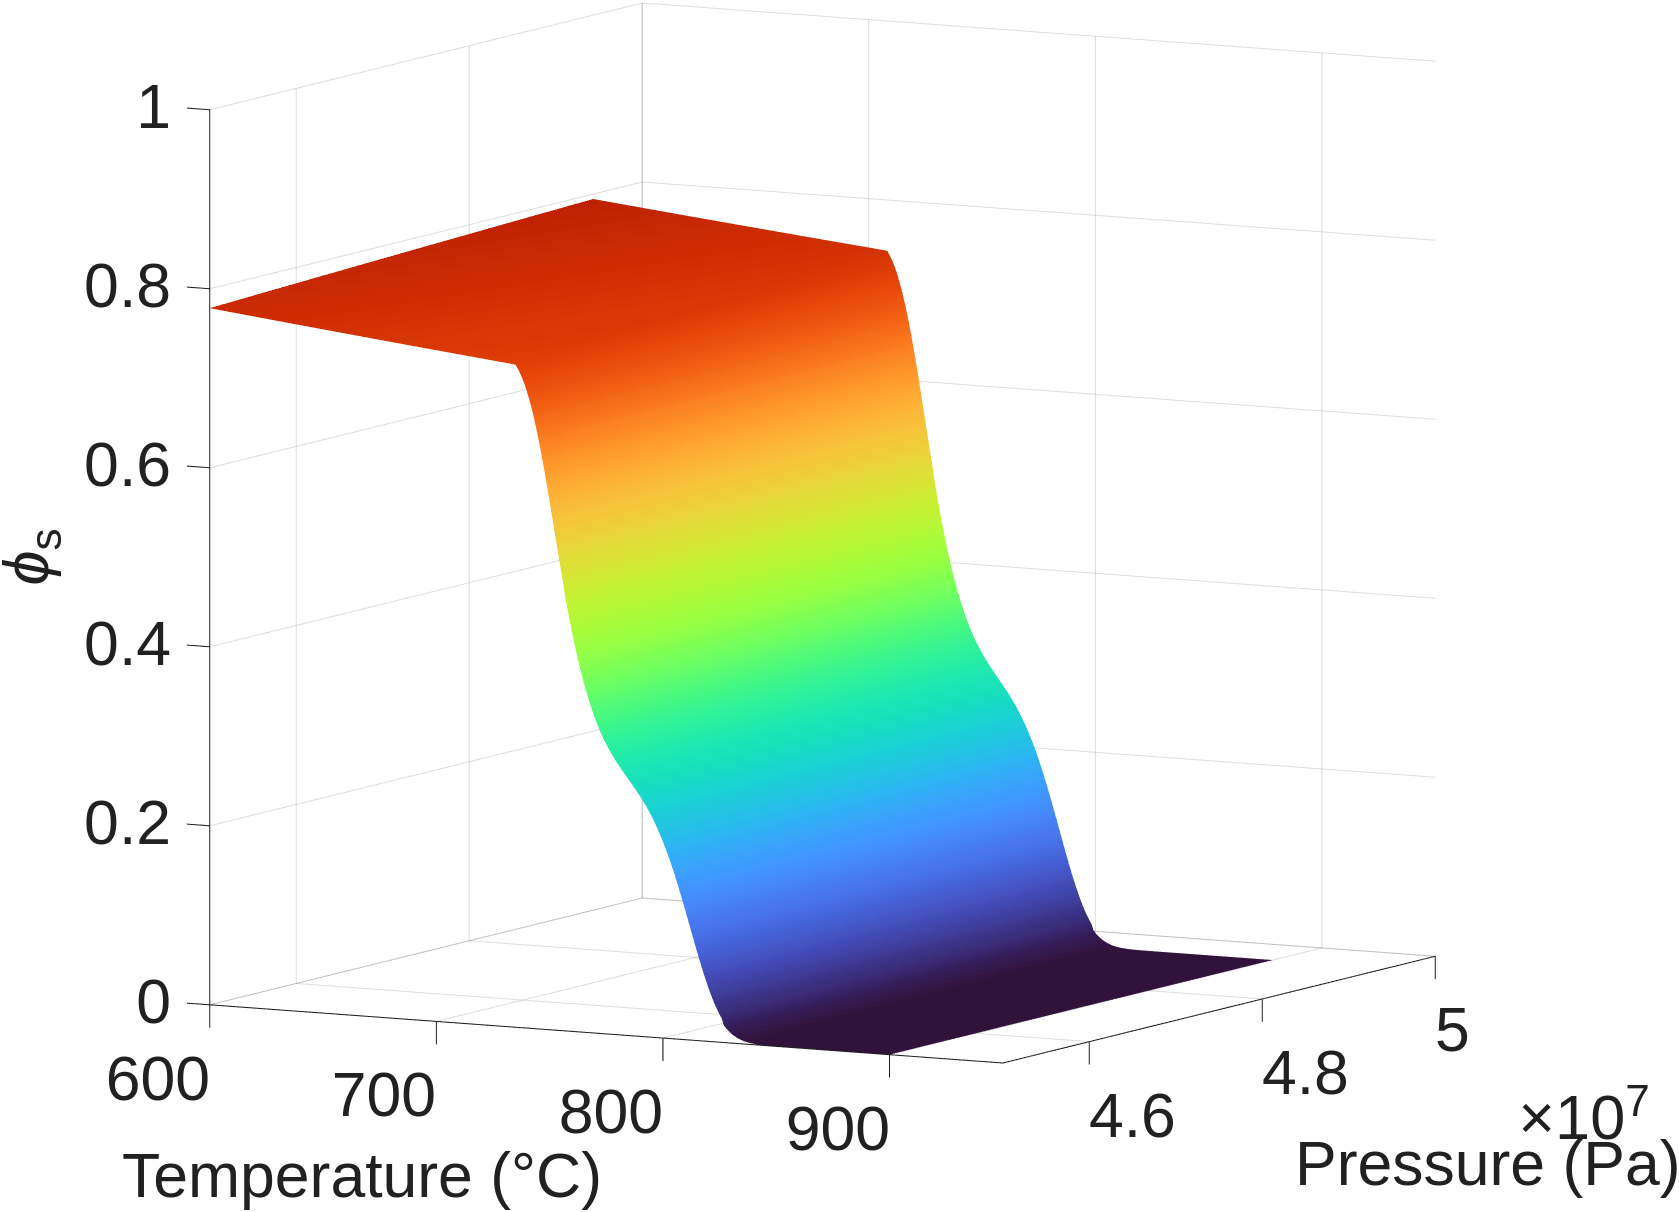
\includegraphics[width=1\linewidth]{img/chapter2/properties/vf_s/vf_s_3D.png}
    \caption{Bulk thermal conductivity modeled for 45 MPa}
    \label{fig:enter-label}
\end{figure}


\subsubsection{Density}
Density plays a critical role in the physical behavior and thermal evolution of magmas within the Earth's interior. It governs buoyancy-driven processes, such as magma ascent, crystal settling, magma mixing and melt segregation, which in turn influence magma chamber dynamics, volcanic eruptions, and the formation of igneous rock textures. Magma density is not constant, it varies with temperature, pressure, chemical composition (notably silica content), and volatile content (especially water and carbon dioxide). Typically, more mafic magmas are denser than felsic ones due to their higher iron and magnesium contents. As magmas cool and crystallize, the residual melt becomes more evolved and less dense, since it gets depleted in heavy elements, often leading to gravitational stratification. Additionally, the exsolution of volatiles during decompression reduces magma density, enhancing buoyancy and potentially triggering eruptions and magma mixing of deeper, more primitive, volatile rich magmas with shallower, evolved and partially degassed magmas. Overall, density controls the mechanical stability and dynamics of magma reservoirs, influencing how magmas differentiate, interact, and ultimately reach the surface.

In our model, melt density is pressure, temperature and composition dependent, obtained from the molar volume expression in \cite{lange1990}:

\begin{equation}
    V_{liq}(T,P,X_i) = \sum X_i \bigg[V_i + \frac{dV_i}{dT} (T-1673) + \frac{dV_i}{dP}(P-10^5)\bigg]
\end{equation}
\begin{equation}
    \rho = \frac{M_{liq}}{V_{liq}}
\end{equation}
where $V_{liq}$ and $M_{liq}$ are the molar volume and mass of the melt, which depend on the oxide composition. $X_{liq}$, $\frac{dV_i}{dT}$ and $ \frac{dV_i}{dP}$ the molar fraction, thermal expansion and compressibility coefficients of the $i_{th}$ oxide. The later are calculated from the data in \cite{lesher2015}.
The density of the exsolved volatile phase, which includes water and carbon dioxide, is computed with the equation of estate from SOLWCAD (\cite{papale2006}) for consistency.

\subsubsection{Heat capacity}
The heat capacity of a substance describes how much energy is required to rise the temperature of a unit of mass of said substance by one degree. It strongly governs the thermal evolution of magmatic systems by controlling how much heat magmas store and release during any process that depends upon temperature such us cooling, heating, crystallization os assimilation. Magmas with higher heat capacities, typically those with higher silica and volatile contents, can absorb more thermal energy without undergoing rapid temperature changes, leading to longer cooling times and more stable magma chambers. During crystallization, the specific heat capacity of the residual melt often increases due to the changes in composition, affecting the thermal gradient and the solidification rate.

Our model computes the specific heat capacity as the weighted average of the different oxide's heat capacities, which are obtained from \cite{lesher2015}, accounting the dissolved water:
\begin{equation}    
    cp_{melt} = \sum_{i=1}^L w_i cp_i + w_{H_2O} cp_{H_2O}
\end{equation}

Heat capacity of the gas phase is temperature dependent, obtained from a regression from classical engineering books, for both components, water and carbon dioxide:

\begin{equation}
\begin{split}
H_2O: &\; 1840.4 - (0.14972 \cdot T) + (9.145 \times 10^{-4} \cdot T^2) \\
&\quad - (3.1759 \times 10^{-7} \cdot T^3) \\
CO_2: &\; 472.27 + (1.5228 \cdot T) - (1.014 \times 10^{-3} \cdot T^2) \\
&\quad + (2.5368 \times 10^{-7} \cdot T^3)
\end{split}
\end{equation}

Mineral heat capacities are modeled after (burman...):

\begin{equation}
\begin{aligned}
cpx_{cp} &= \frac{305.41 - 1604.9\, T^{-0.5} - 7.166 \times 10^6\, T^{-2} + 9.2184 \times 10^8\, T^{-3}}{0.24855} \\[2ex]
kfpr_{cp} &= \frac{381.37 - 1941\, T^{-0.5} - 1.20373 \times 10^7\, T^{-2} + 1.83643 \times 10^9\, T^{-3}}{0.27833} \\[2ex]
qtz_{cp} &= \frac{80.01 - 240.3\, T^{-0.5} - 3.5467 \times 10^6\, T^{-2} + 4.9157 \times 10^8\, T^{-3}}{0.06008} \\[2ex]
plg_{cp} &= \frac{393.64 - 2415.5\, T^{-0.5} - 7.8928 \times 10^6\, T^{-2} + 1.07064 \times 10^9\, T^{-3}}{0.26222} \\[2ex]
mgt_{cp} &= \frac{235.90 - 1766.6\, T^{-0.5} - 1.7104 \times 10^6\, T^{-2} + 4.062 \times 10^8\, T^{-3}}{0.23153}
\end{aligned}
\end{equation}

\begin{figure}[H]
    \centering
    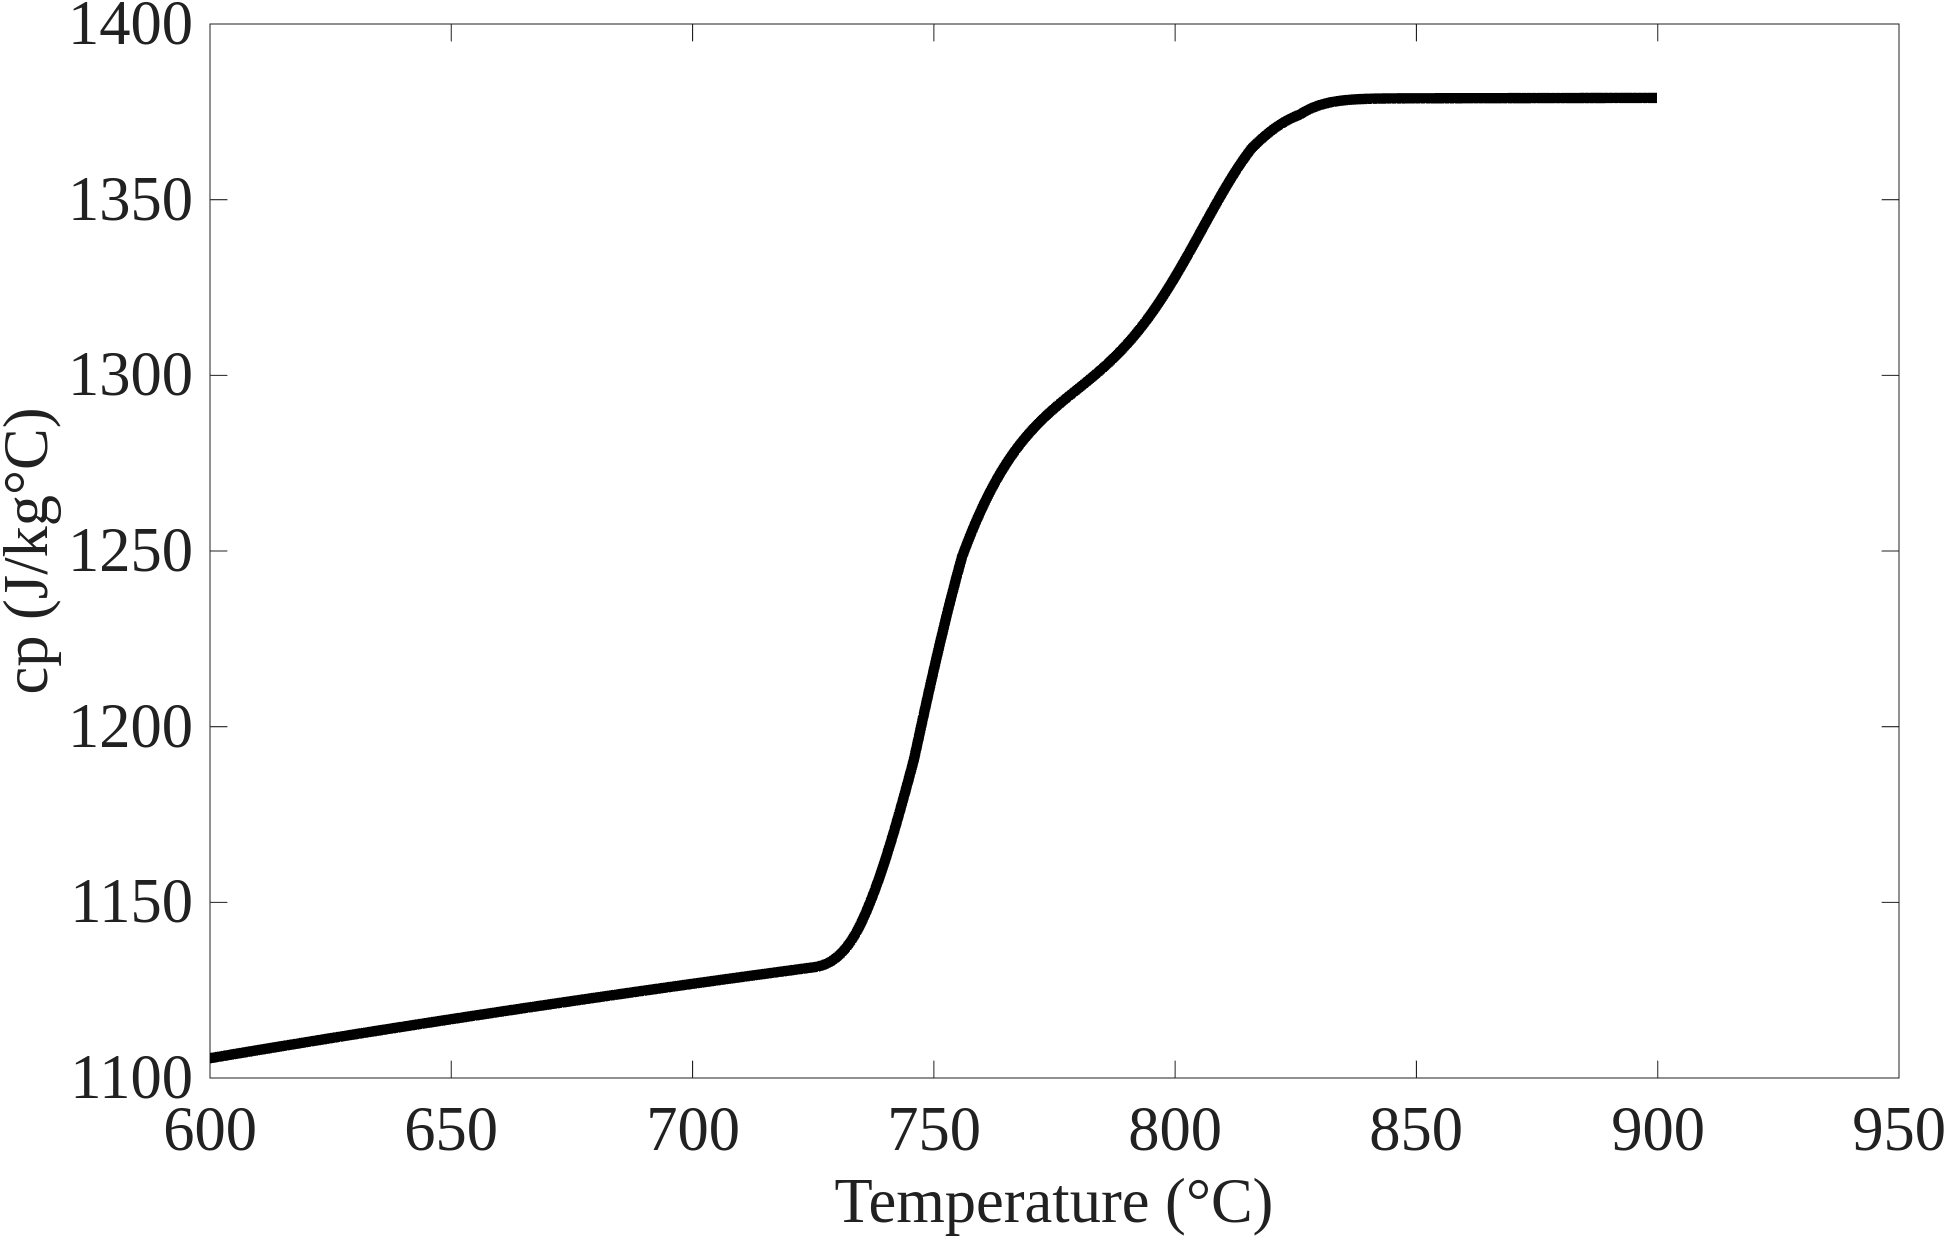
\includegraphics[width=1\linewidth]{img/chapter2/properties/heat_capacity/SMOOTHED_cp.png}
    \caption{Bulk heat capacity modeled for 45 MPa}
    \label{fig:enter-label}
\end{figure}

\subsubsection{Thermal conductivity}
Thermal conductivity can be defined as how efficiently heat is transmitted through any substance by molecular or lattice vibrations. It is a crucial parameter that strongly controls the rate of heat loss from magma to surrounding rocks, which influences cooling rates, crystallization times, and overall magma chamber stability. Generally, magmas have relatively low thermal conductivity compared to solid rocks, due to their disordered liquid structure and high temperatures. This low conductivity causes magmas to efficiently retain heat, contributing to the long-lived nature of magma chambers. As crystallization advances, thermal conductivity normally increases due crystals higher thermal conductivity when compared to melt. Additionally, variations in composition, crystal content, and volatile phases can cause anisotropy in thermal transport, affecting localized cooling paths and magma differentiation.

Thermal conductivity of the melt is calculated from the thermal diffusivity definition from \cite{moitra2018}
\begin{equation}
\begin{split}
&\alpha_L = (-0.06 + 4.57*T)\times 10^{-6}\\
&\kappa_L = \rho_L cp_L \alpha_L\\
\end{split}
\end{equation}
With the equation of \cite{heap2020} we calculate the thermal conductivity of combined mixture of crystals and melt.
\begin{equation}
\begin{split}
&\kappa_D = \frac{\kappa_L(1-\phi_c)(1-m_c) + m_c \beta_c \phi_c}{(1-\phi_c)(1-m_c) + \beta_c \phi_c}\\
&m_c = \frac{\kappa_c}{\kappa_L} \qquad \beta_c = \frac{3(1-m_c)}{2+m_c}
\end{split}
\end{equation}
Gas thermal conductivity is calculated from a regression of data and \cite{udoetok2013} equation for binary mixtures of gases:   
\begin{equation}
\begin{split}
&\kappa_G = \frac{1}{2}\bigg[\frac{\kappa_{H_2O}\kappa_{CO_2}}{\chi_{H_2O}\kappa_{H_2O} + \chi_{CO_2}\kappa_{CO_2}}\bigg] \\
&\quad +\chi_{H_2O}\kappa_{H_2O} + \chi_{CO_2}\kappa_{CO_2}\\
\\&\kappa_{H_2O} = 4.1771\times 10^{-3} + 2.2849\times 10^{-5}*T \\
&\quad + 9.4663\times 10^{-8} * T^2 - 2.5778\times 10^{-11} * T^3\\
\\&\kappa_{CO_2} = -1.0081\times 10^{-3} + 9.1422\times 10^{-5}*T \\
&\quad - 6.4318\times 10^{-8} * T^2 - 4.31\times 10^{-11} * T^3\\
\end{split}
\end{equation}
where $\chi_{H_2O}$ and $\chi_{CO_2}$ are the molar concentration of each component in the total gas mixture. Similarly to how it is done for the crystal and magma dense phase, we compute the bulk thermal conductivity for the dense phase plus gas phase using equation (14).

\begin{figure}[H]
    \centering
    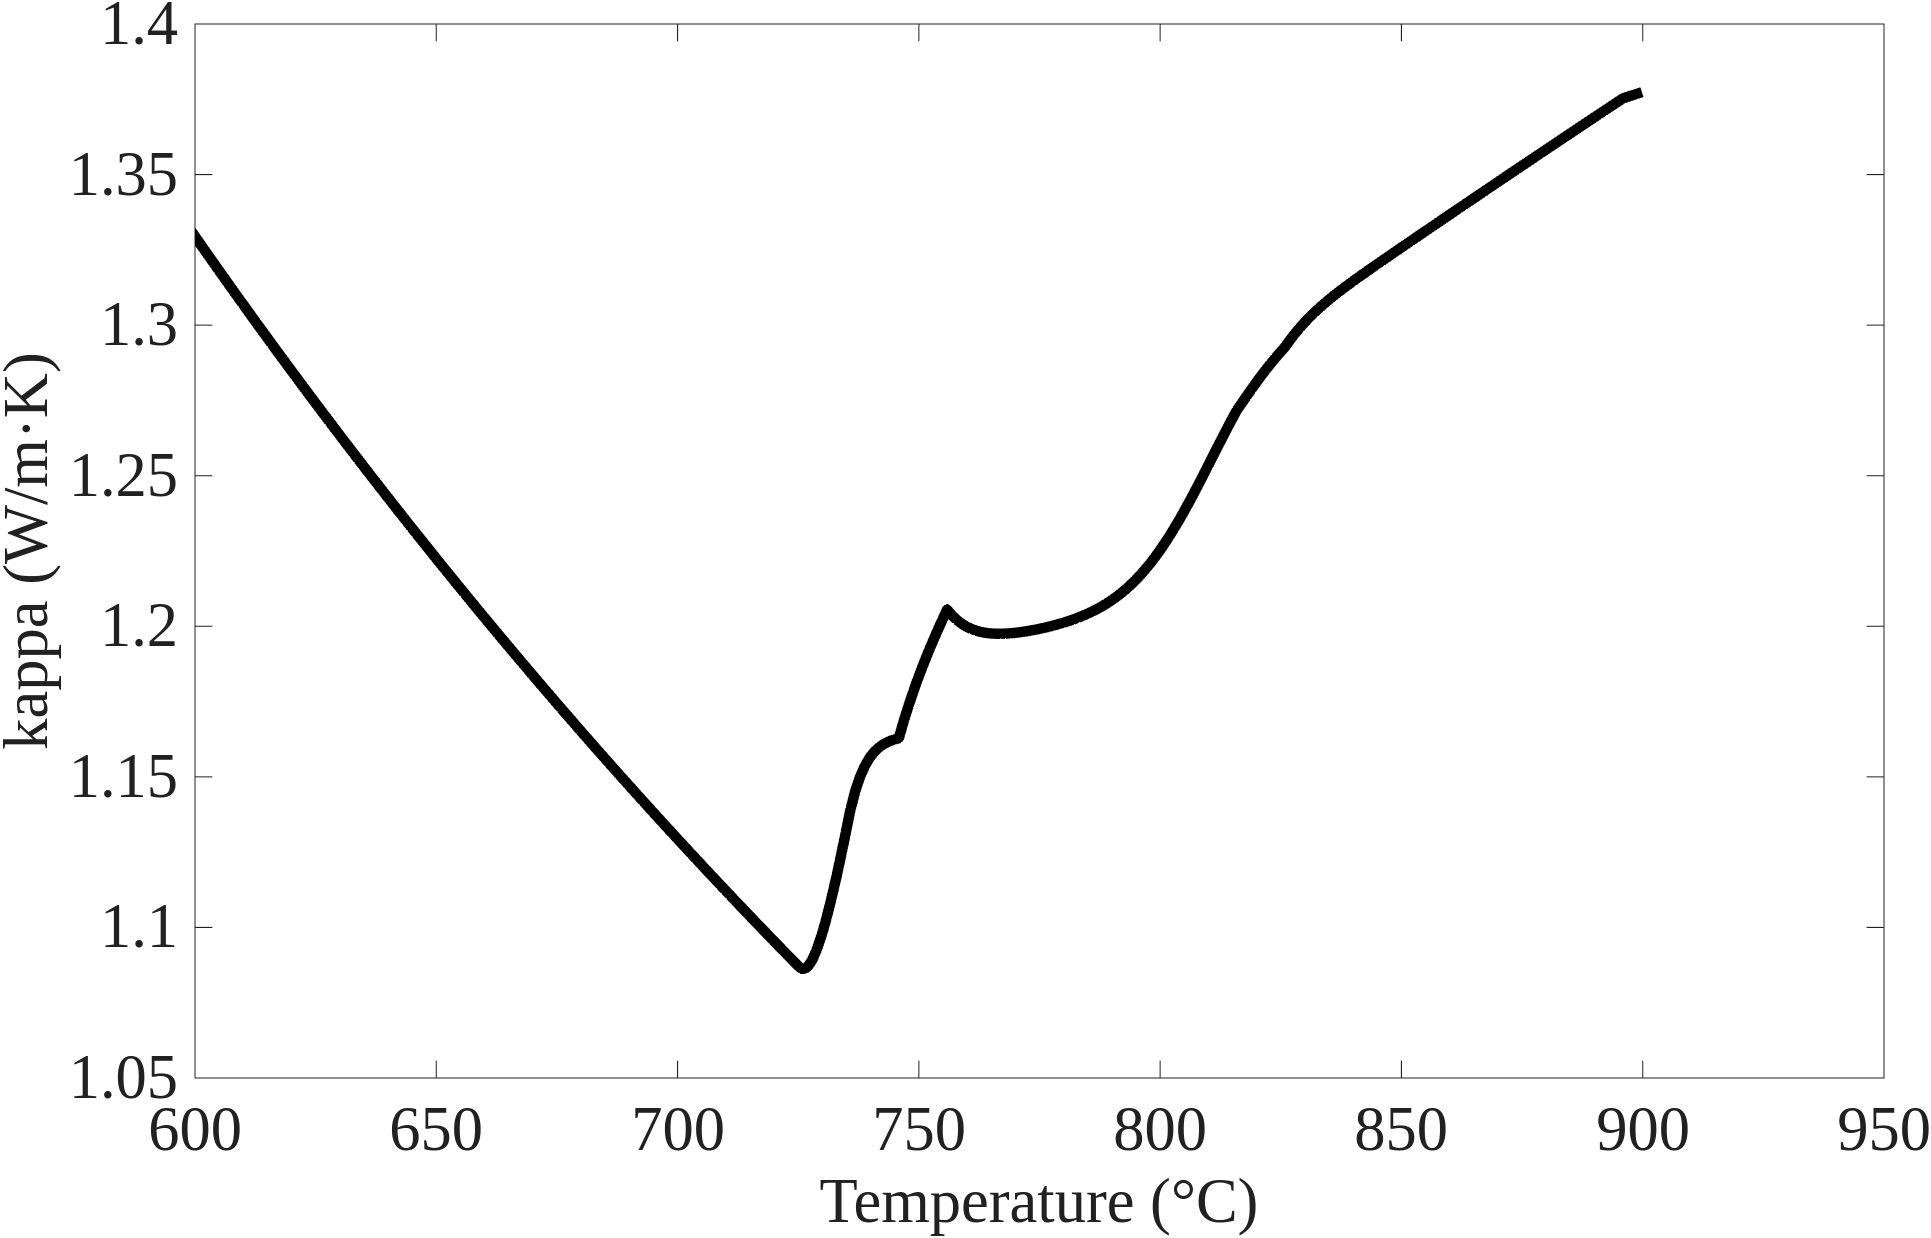
\includegraphics[width=1\linewidth]{img/chapter2/properties/kappa/SMOOTHED_kappa.png}
    \caption{Bulk thermal conductivity modeled for 45 MPa}
    \label{fig:enter-label}
\end{figure}

\subsubsection{Viscosity}
Viscosity is one of the most critical physical properties of magma, which exerts major control on its flow behavior, eruption dynamics, crystallization history and many more processes. In simple words, it measures a fluid's resistance to flow and deformation. Viscosity of magmas is highly sensitive to temperature, composition and crystal and volatile content. Silica-rich magmas such as rhyolite have, generally, much higher viscosity than silica-poor, such as basalt, due to its higher state of polymerization of the silica tetrahedra within the melt. As magmas cool, viscosity increases exponentially due to the combined effect of higher polymerization and crystallization. This can strongly influence magma behavior, slowing down convection o favoring mush formation, and have a profound effect on its eruptive behavior, ranging from tranquil, effusive eruptions to violent and explosive ones with increasing viscosity, as gas bubbles struggle to coalesce and easily scape, and, as opposed, get over-pressurized. The effect of volatiles is less clear and more varied: higher dissolved volatiles content decreases magma viscosity, but exsolved bubbles can behave as rigid, non-deformable particles, hence increasing viscosity, or like deformable objects, decreasing viscosity.

In order to compute de viscosity of the system we need to account at any time and in any point in space for the combined effect of all the coexisting phase, as well as the strain rate. Due to the complexity of such system, a model that is able to able to approximate the viscosity accounting for the contribution of all these variables is yet non existent. Therefore, we tackle this issue as follows: first we compute the Newtonian viscosity according to the well known and widely used model by \cite{giordano200} and add to this viscosity the effect of crystals and strain rate applying the model by \cite{caricchi2007}, described as follows:

\begin{equation}
\eta_r(\phi) = \frac{1 + \big(\frac{\phi}{\phi_{\text{max}}}^{\delta}\big)}
{\bigg(1 - \alpha \, \text{erf} \bigg\{ \frac{\sqrt{\pi}}{2a} \frac{\phi}{\phi_{max}}
\bigg[ 1 + \bigg(\frac{\phi}{\phi_{max}}\bigg)^\gamma \bigg] \bigg\}\bigg)^{\gamma \phi_{\text{max}}}}
\end{equation}

where B is the Einstein coefficient (\cite{einstein1905}) with a value of 2.5. The rest of the parametres are calculated from the following relations:

\begin{equation}
    \begin{aligned}
        \phi_{max} = 0.066499·tanh(0.913424)·log_{10}(\dot{\gamma}) + 3.850623 + 0.591806 \\
        \delta =-6.301095·tanh(0.818496·log_{10}(\dot{\gamma}) + 2.86 + 7.462405 \\
        \alpha = 0.000378·tanh(1.148101·log_{10}(\dot{\gamma}) +3.92+0.999572 \\
        \gamma = 3.987815·tanh(0.8908·log_{10}(\dot{\gamma} + 3.24 + 5.099645)        
    \end{aligned}
\end{equation}

To this mixture of melt and crystals we then add the contribution of gas bubbles with the also strain rate dependent model of \cite{llewellin2005}, a simplification of the model by \cite{pal2003}, which defines two regimes depending on the capillary number: with capillary numbers larger than 1, viscosity increases with the increase of the gas volume fraction, as bubbles behave rigidly. On the other hand, the second regime occurs when the capillary number is smaller than 1: bubbles are able to deform, hence, shear viscosity decreases with increasing volume fraction of gas. The capillary number can be expressed as follows:

\begin{equation}
    Ca = \frac{R\eta\dot{\gamma}}{\sigma}
\end{equation}
 where R is the bubble radius, $\eta$ is the viscosity of the melt+crystals mixture, $\dot{\gamma}$ is the strain rate and $\sigma$ is the surface tension.

\cite{llewellin2005} reduce the model by \cite{pal2003} to more simple expression: 

\begin{equation}
    \begin{aligned}
        \text{If Ca < 1} \ \ \ \ \ \ \ \ \eta_r=(1-\phi_g)^{-1} \\
    \text{If Ca $\geq$ 1} \ \ \ \ \ \ \ \ \eta_r=(1-\phi_g)^{\frac{5}{3}}
    \end{aligned}
\end{equation}
 
where $\phi_g$ is the volume fraction of the gas phase. 
Once obtained the relative viscosity applying the effect of the gas phase, the total viscosity of the system can be easily obtained by multiplying this relative viscosity with the viscosity of the melt+crystals mixture. In addition, and for numerical stabuility and convergence it is necessary to fix the maximum viscosity to $10^{13}$ Pa$\cdot$s.


% \begin{figure}
%     \centering
%     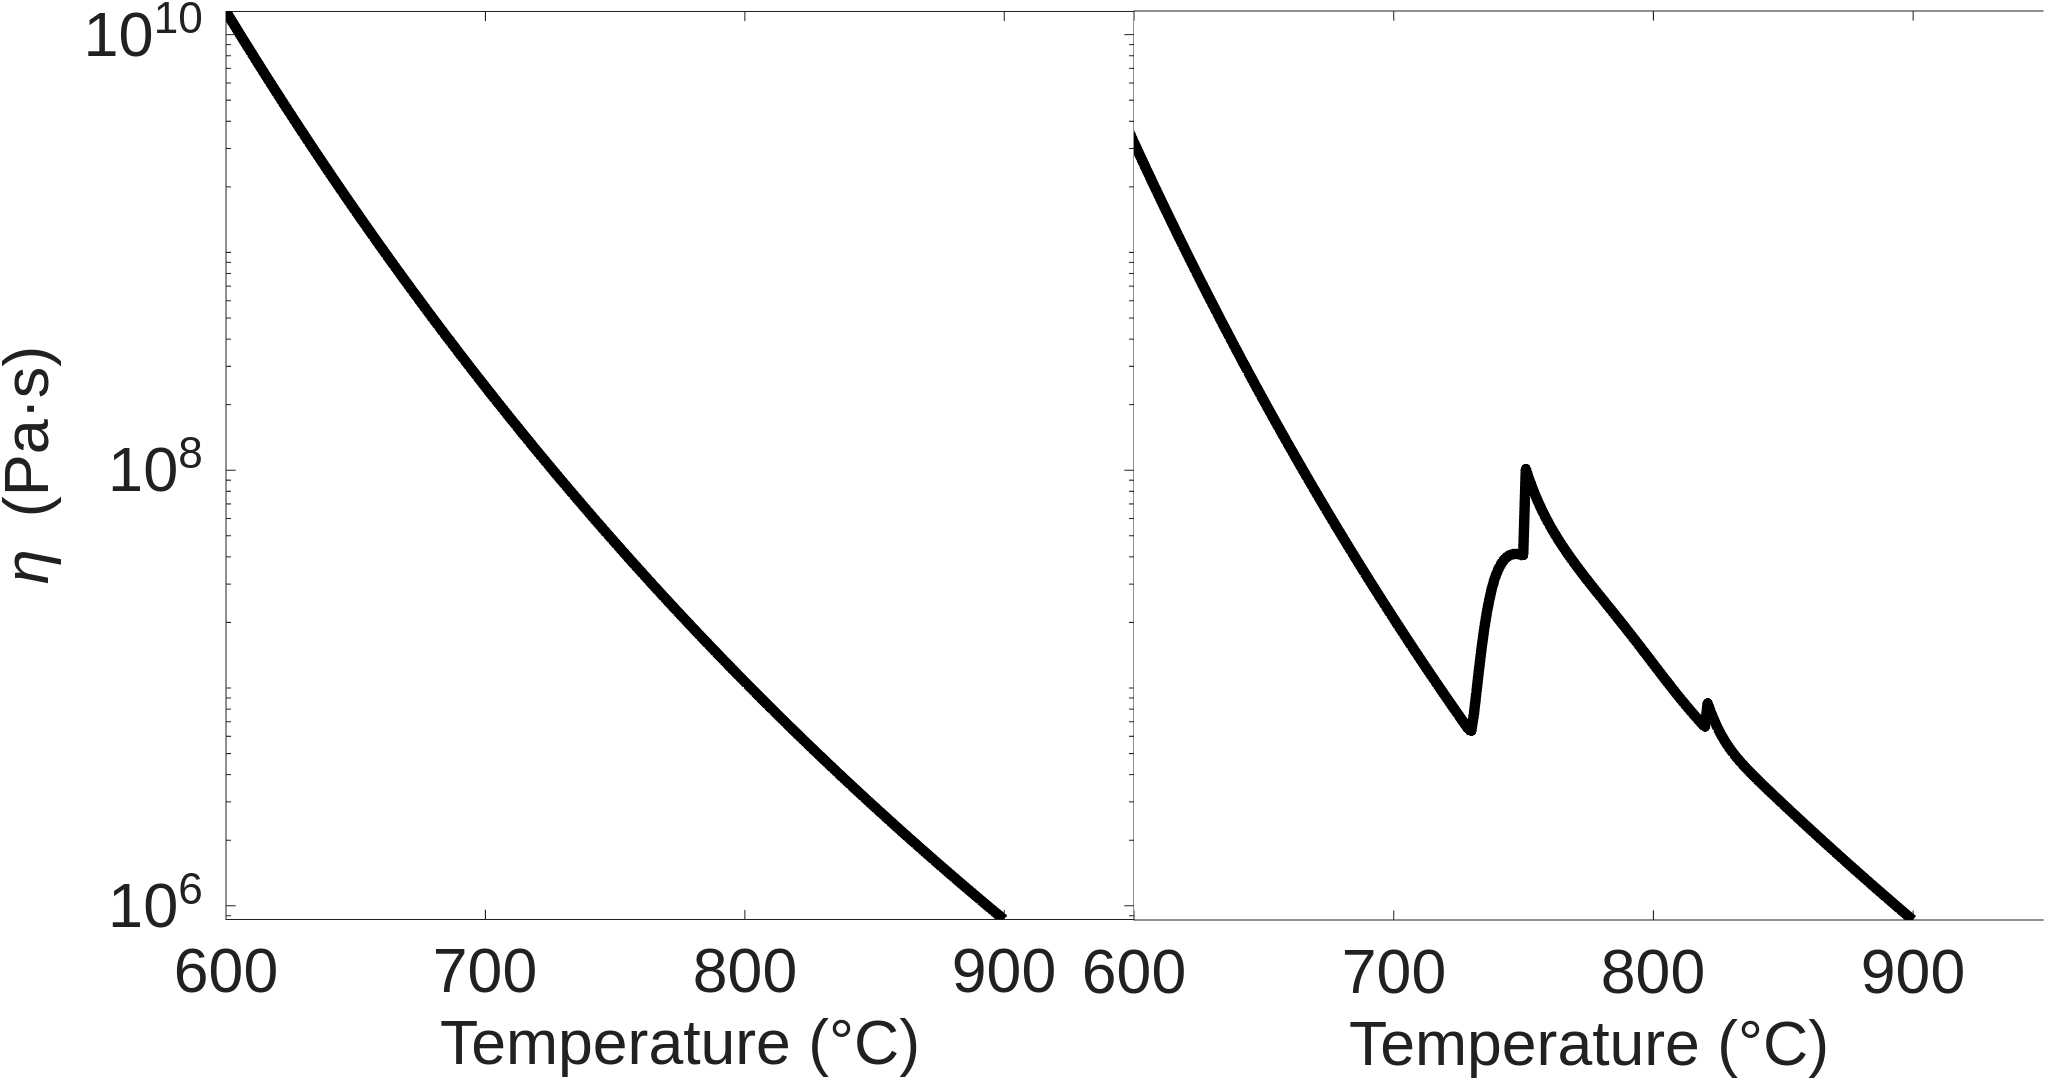
\includegraphics[width=1\linewidth]{img/chapter2/properties/viscosity/newtonian_square_30font_merged.png}
%     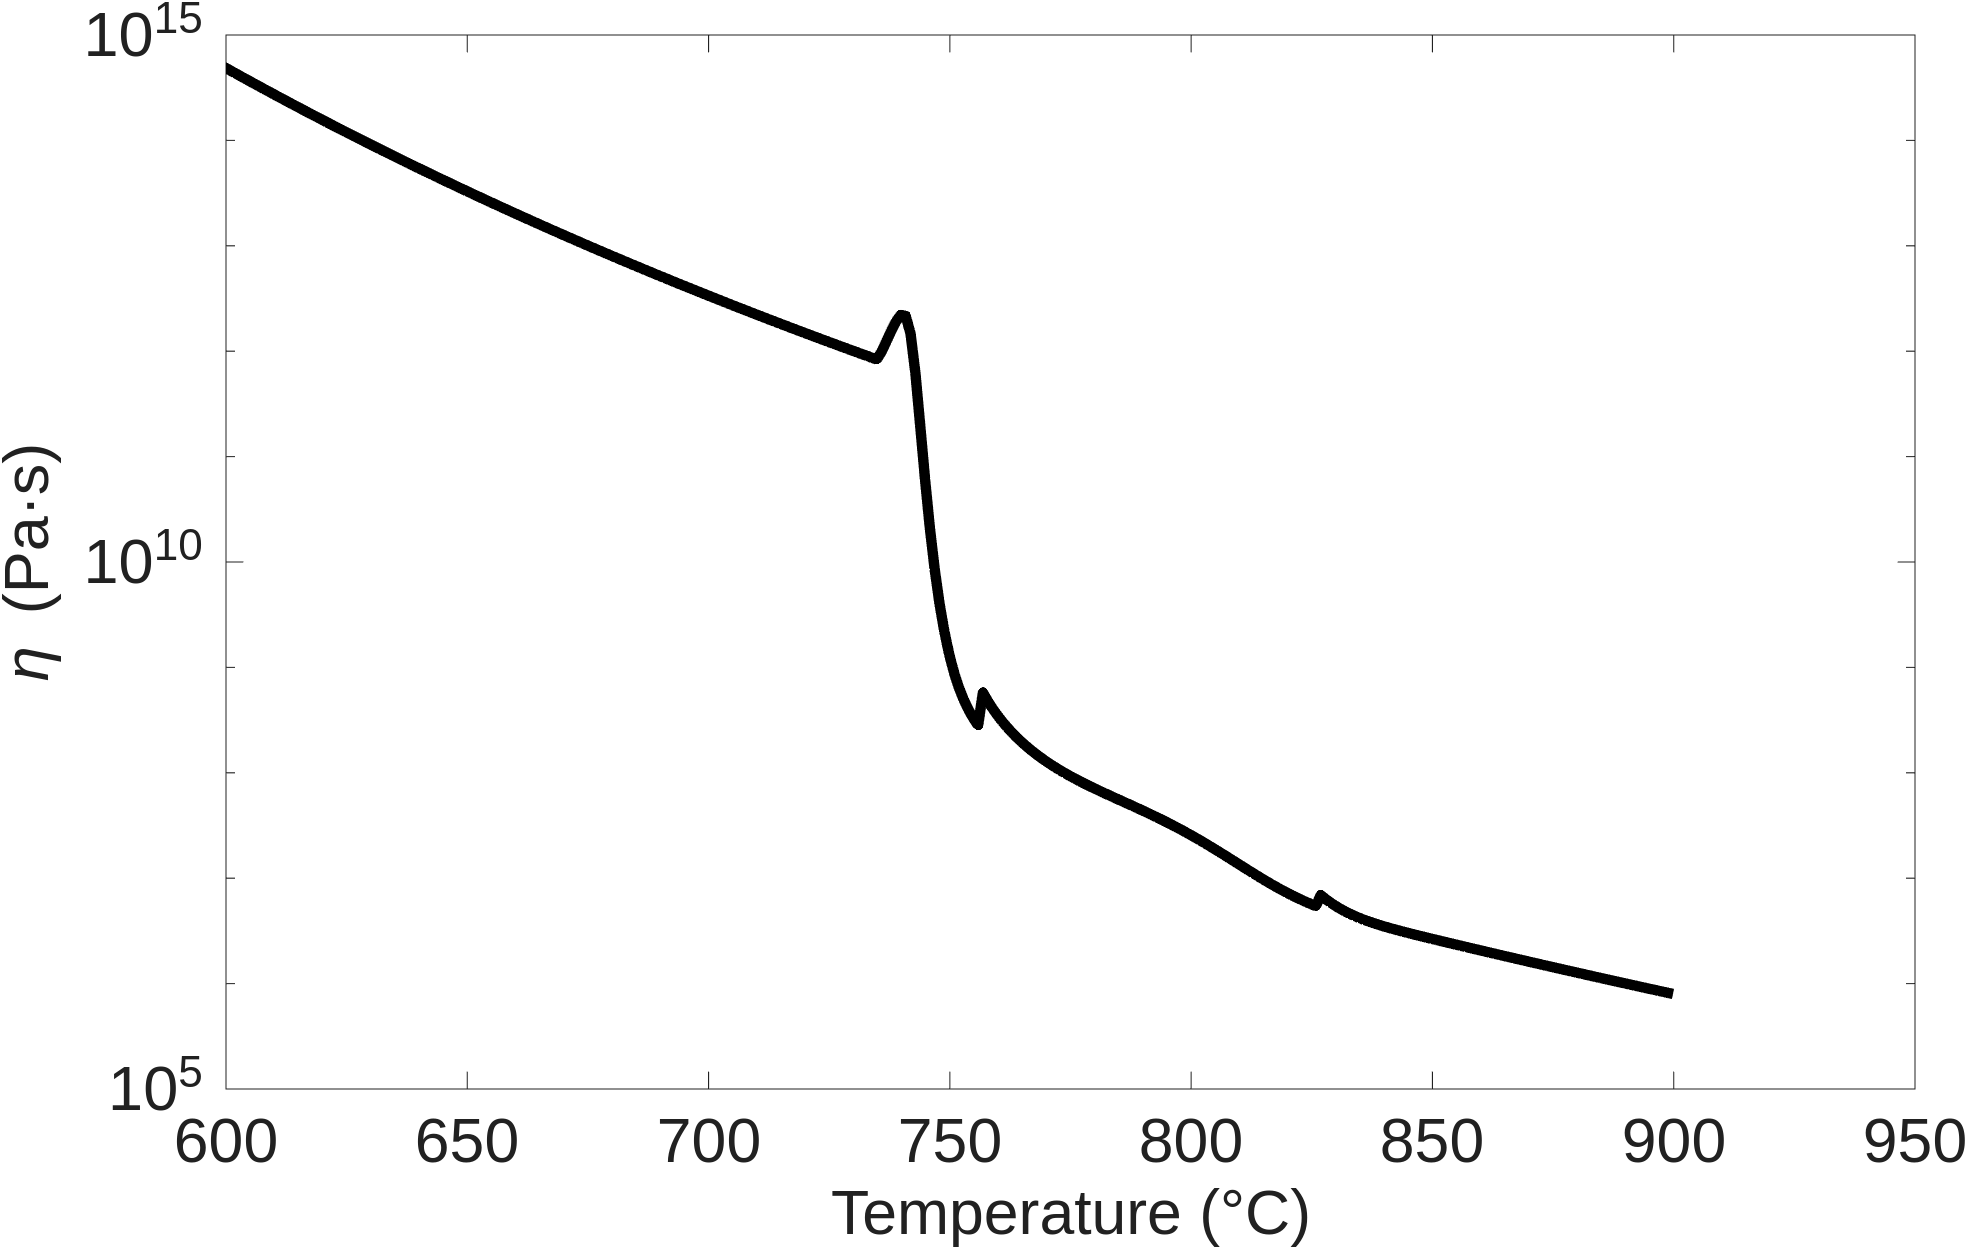
\includegraphics[width=1\linewidth]{img/chapter2/properties/viscosity/non_newt_full.png}
%     \caption{Temperature field for the 2D convection 1c benchmark once it has reached the final steady state stage}
%     \label{fig:enter-label}
% \end{figure}


\begin{figure}
    \centering

    \begin{tikzpicture}
        \node[inner sep=0pt] (img1) at (0,0) {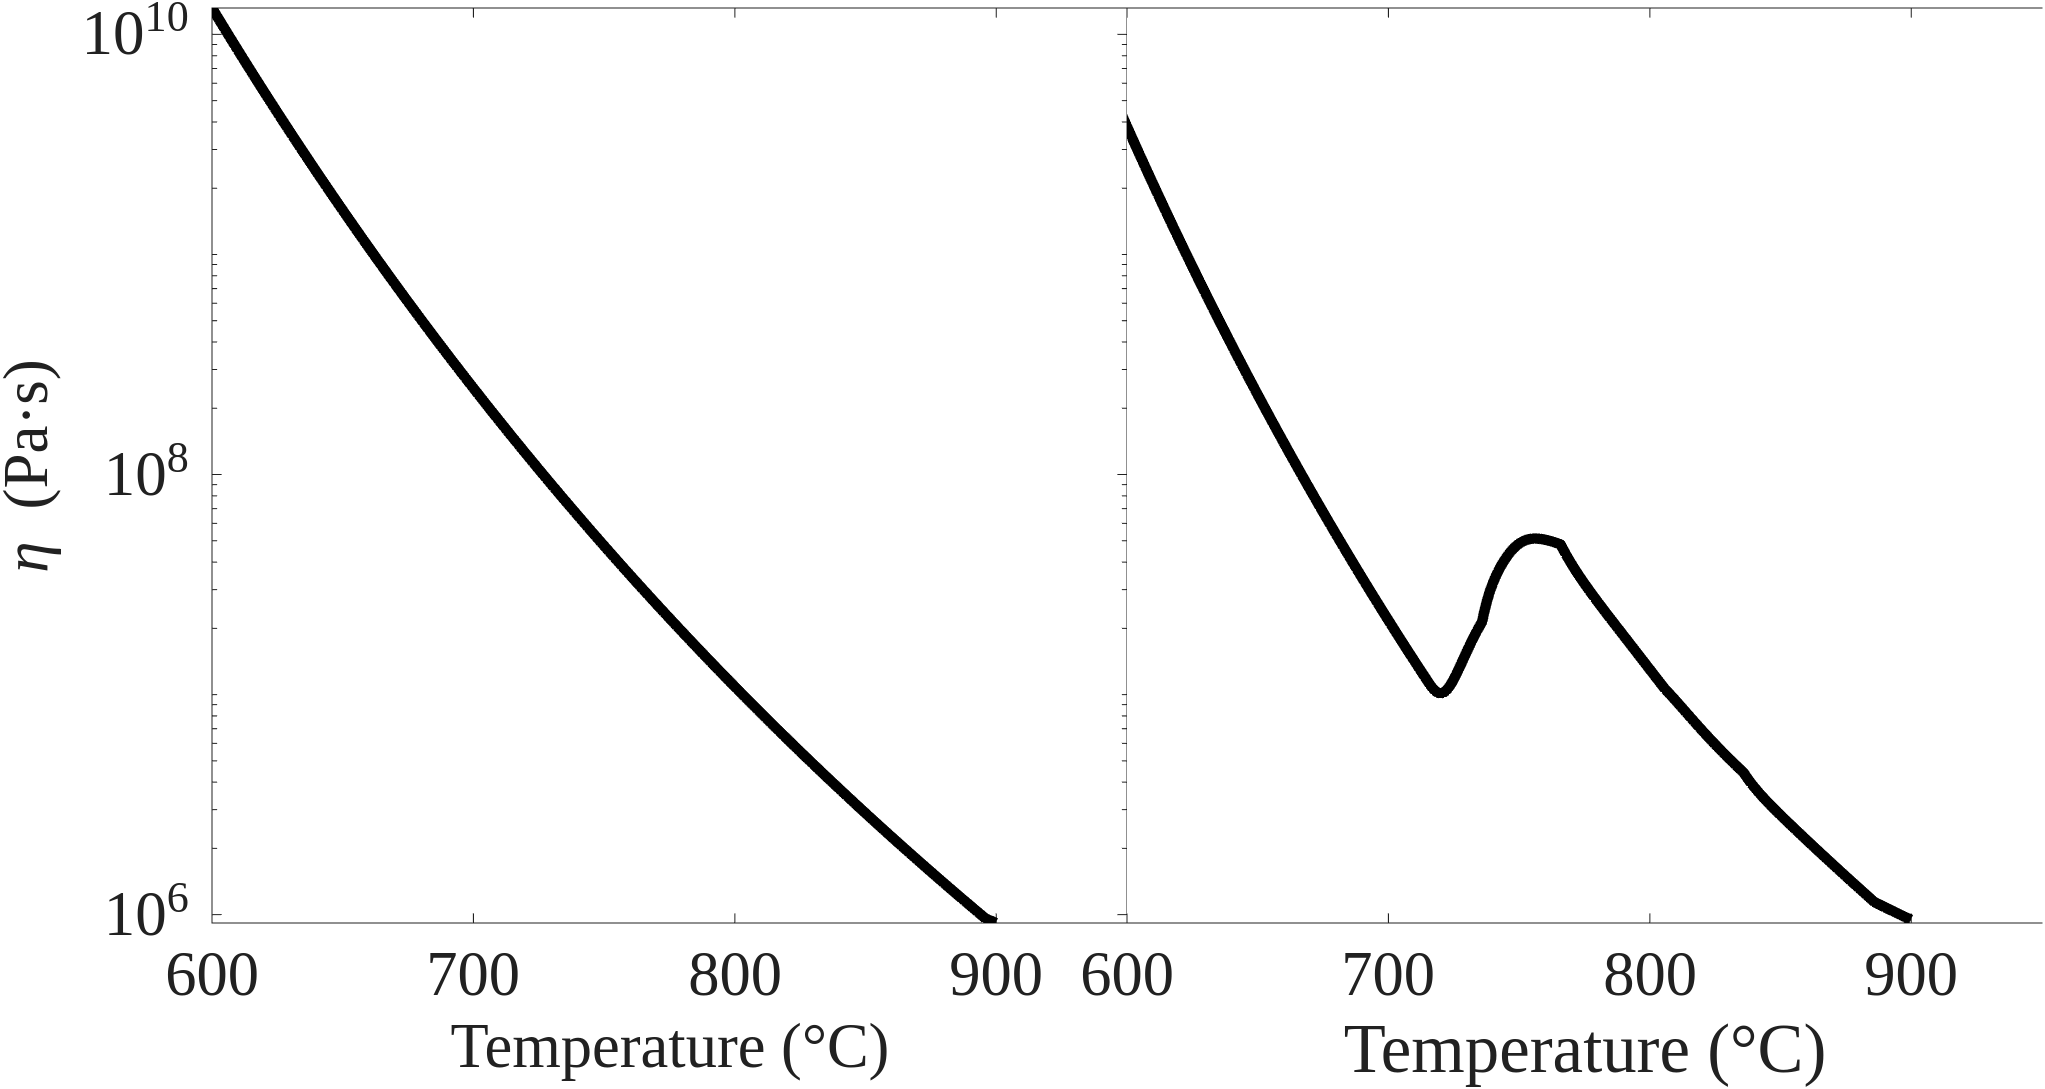
\includegraphics[width=1\linewidth]{img/chapter2/properties/viscosity/SMOOTHED_newtonian_square_30font_merged_1.png}};
        \node[anchor=north east, xshift=-8pt, yshift=-5pt] at (img1.north east) {\textbf{(a)}};
    \end{tikzpicture}
    \begin{tikzpicture}
        \node[inner sep=0pt] (img2) at (0,0) {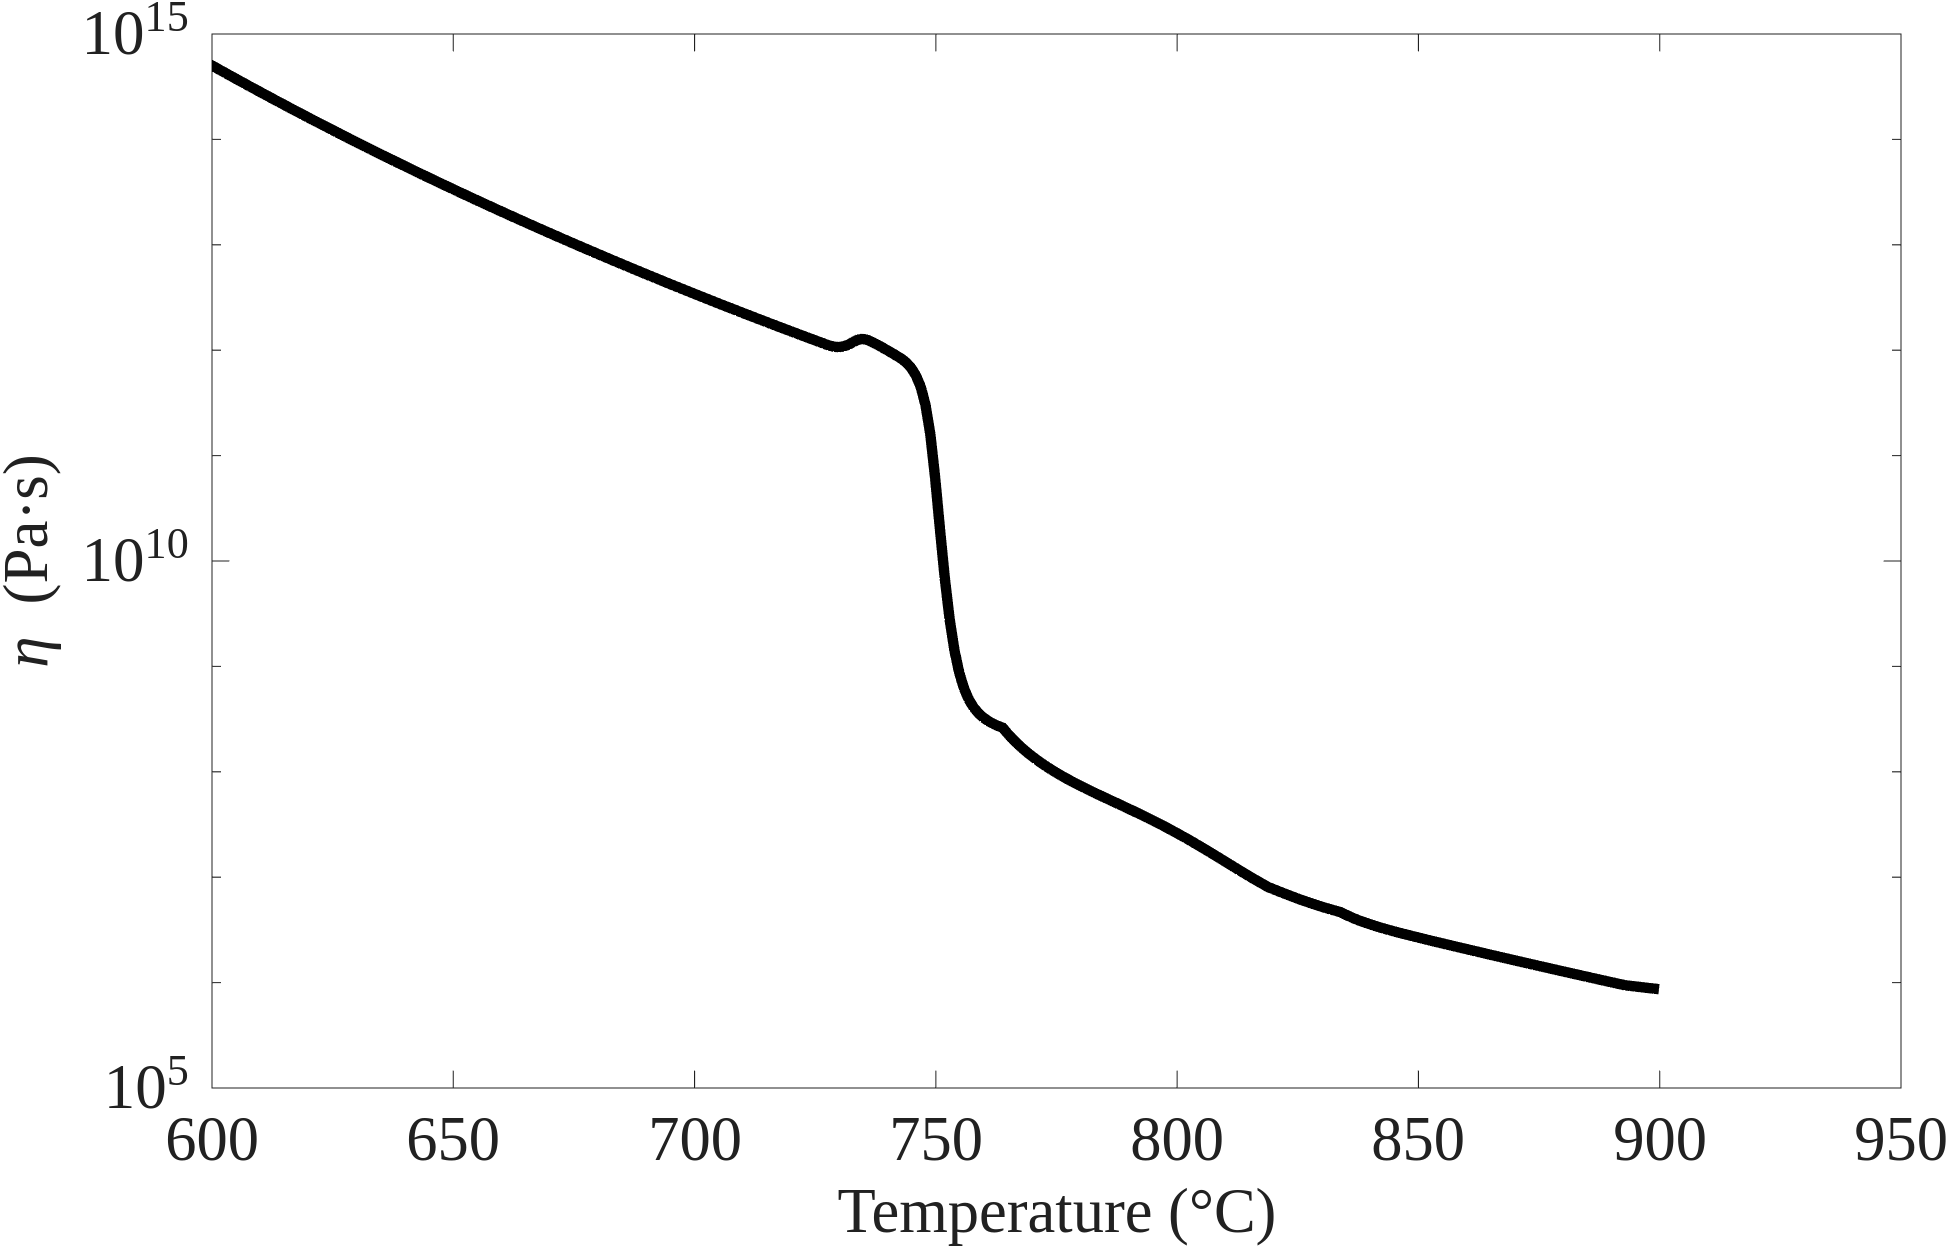
\includegraphics[width=1\linewidth]{img/chapter2/properties/viscosity/SMOOTHED_non_newt_full.png}};
        \node[anchor=north east, xshift=-8pt, yshift=-5pt] at (img2.north east) {\textbf{(b)}};
    \end{tikzpicture}

    \caption{Temperature field for the 2D convection 1c benchmark at final steady state.}
    \label{fig:2d-convection-temp}
\end{figure}


\begin{figure}
    \centering
    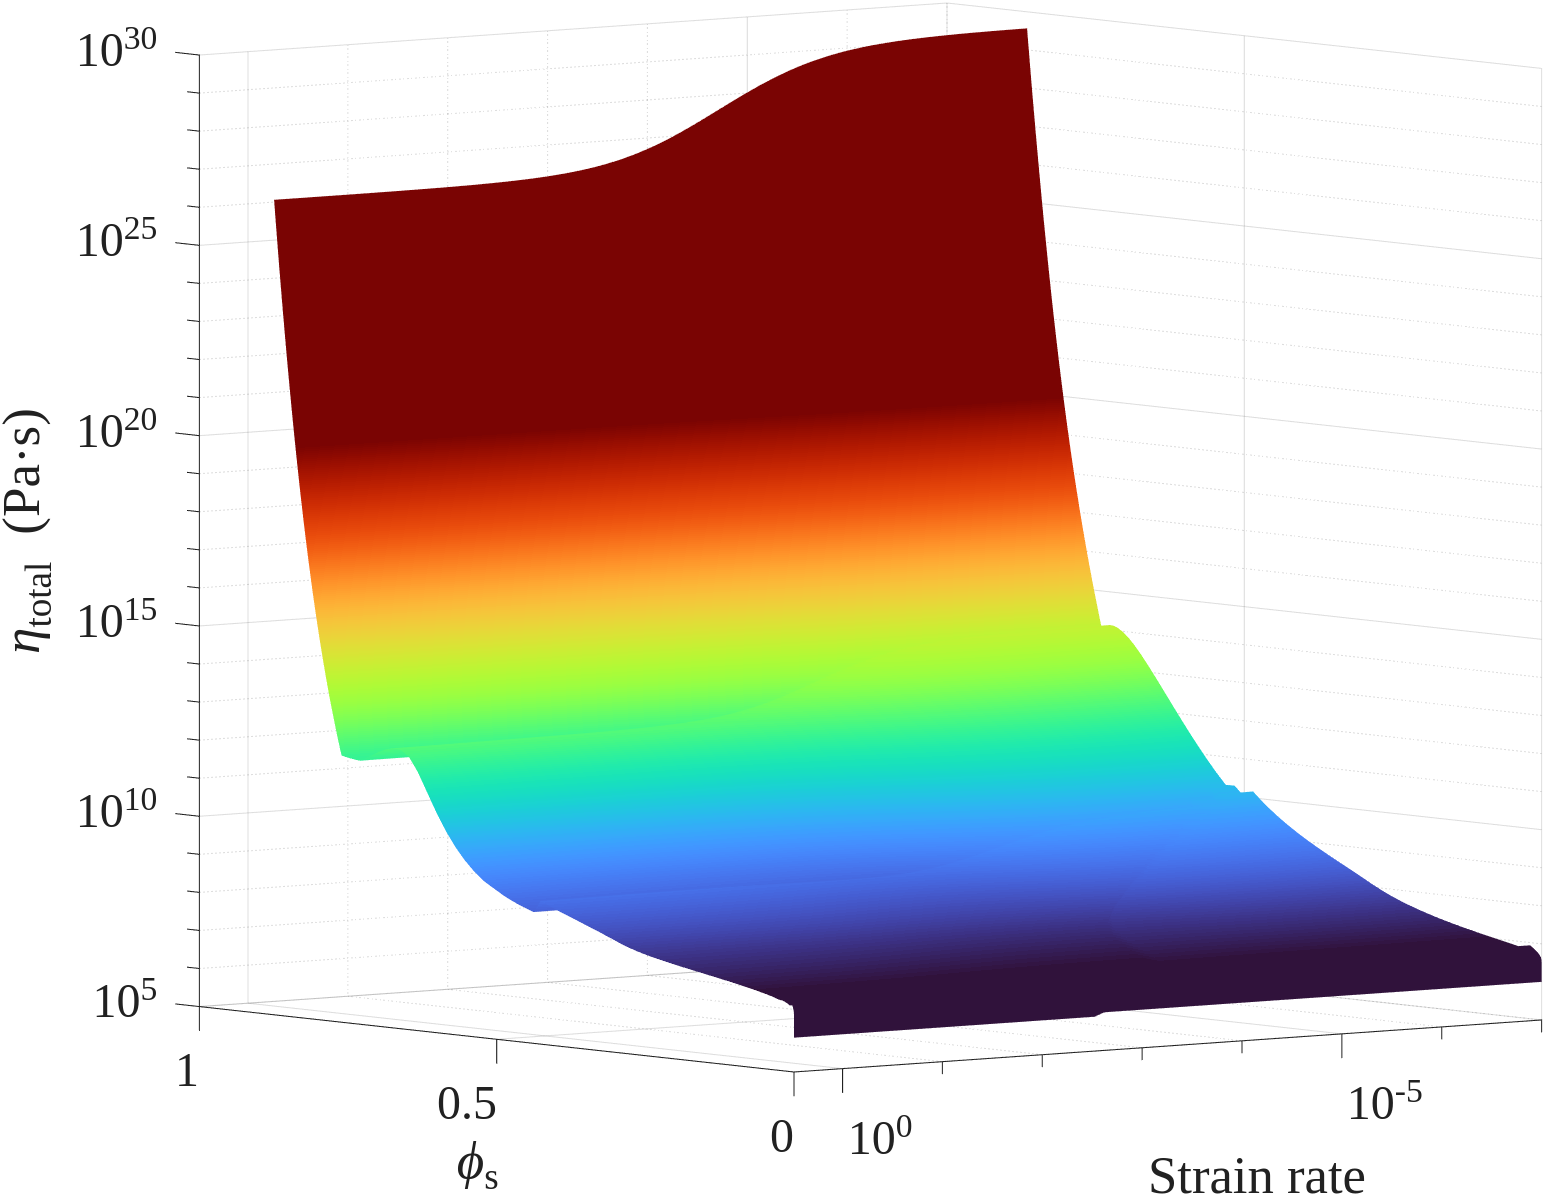
\includegraphics[width=1\linewidth]{img/chapter2/properties/viscosity/non_newt_3D_phi.png}
    \caption{Temperature field for the 2D convection 1c benchmark once it has reached the final steady state stage}
    \label{fig:enter-label}
\end{figure}

\subsubsection{Latent heat}
Latent heat of phase change can be described as the amount of energy that is supplied of extracted from a substance in order to change its state at constant temperature and pressure. Within the context of magma kinetics, it is the heat released when a crystal is formed from the melt, or the heat absorbed by the melt when a volatile particle is exsolved. It is a fundamental magmatic process. Its influence on the energy balance of magmatic regions has being extensively studied. It partially or totally controls diverse processes that strongly affect magma emplacement, evolution and migration. \cite{depaolo1981}, \cite{huppert1988}, \cite{spera2001}, \cite{tavazzani2024} state that primitive magmatic intrusions release enough heat during crystallization to induce partial melting of the crustal rocks. \cite{anne2005}, \cite{blundy2006}, \cite{dufek2010}, \cite{namur2014}, \cite{newcombe2020}, among many others state the importance of latent heat of crystallization in buffering magma chambers against fast crystallization, suntanning deep crustal mush zones, and even influencing shallow processes like eruptions, by exerting some control over the temperature evolution during magma the ascent. It is clear then, that latent heat is not something to be overlooked, and it is of the most importance to account for its effect on our numerical simulations. 

As it is the nature itself of the latent heat of phase change, it is added to the heat transfer equation as a source term, since it can be both a source of heat, when crystallizing, or a sink of heat, when reabsorbing mineral phases or exsolving volatiles. The temperature equation is modified as follows:

\begin{equation}
\rho c_p \left(\underbrace{\frac{\partial T}{\partial t}}_{\text{Transient term}} + \underbrace{\mathbf{v} \cdot \nabla T }_{\text{Convection term}}\right) = \underbrace{\nabla \cdot (k \nabla T)}_{\text{Conduction term}} + \underbrace{\sum_{i}^n\rho_iqL_i\phi_{i_{,t}}}_{\text{Latent heat of phase change term}}
\end{equation}

This term is described by the summation of each phase's density ($\rho_i$), its latent heat of phase change ($qL_i$) and the change on its volume fraction ($\phi_i$) with respect to time. The latent heat of phase change is computed for each phase, mineral or gas as the difference between between the heat capacity and the melt, multiplied by the increment in temperature from an standard state:

\begin{equation}
    qL_p = (cp_p-cp_L)(T-T_0)
\end{equation}

where cp$_p$ is the heat capacity of the phase, cp$_L$ is the heat capacity of the melt, T is the current temperature at the calculation point, and T$_0$ is the temperature at the standard state, that we take as 0°K. The value of $qL$ is in the order -250000 $J/Kg$ for the mineral phases and 600000 $J/Kg$ for the gas phase. As in can be expected, this term accounts for the latent heat of crystallization as well as for the heat absorbed by reabsorption or remelting of the phases.


\section{Simulation setup}
In this section, the setup for the main simulations that constitute the core of this work is explained. The simulations aim to be representative of the Krafla system, since the main objective of the work is to analyze and determine the stability conditions of the found magma, including the internal dynamics of the magma. Thus, we design a number of simulations that are representative of the Krafla system, but not only, since the results can potentially explain, hence applied to other potential shallow magmatic bodies in any other part of the world. 

Since the magma pocket, as it has being already mentioned, is yet to be constrained in size and shape by geophysical methods, the approach taken in the present work is a first order and straightforward approximation: a sill-like disk shaped magma chamber and a set of chamber sizes that are arbitrarily chosen, but representative, and of dimensions that are not larger than the resolution of usual geophysical methods, since the body (or bodies) went unnoticed under every geophysical survey that had taken place before the encounter. 

This section presents the magma domain, discussing the geometries of the simulated magmatic bodies and the different set if boundary and initial conditions such as pressure and temperature for each of the chambers. Following, the rock domain is presented in a similar way.
\subsection{Simulation domain}
\subsubsection{Magma domain}
For the magma domain, three sizes are chosen, which are referred as:\textit{small}, \textit{medium} and \textit{large}.
\textit{Small} body's long axis is 782 meters while the short axis is 156 meters. The simulated volume would be $~5*10^7 m^3$. 
Thickness and with of the \textit{medium} body are 336 meters and 1648 meters respectively, adding up to a volume of $~5*10^8 m^3$. 
Lastly, for the \textit{large} body, the dimensions are $2672x534$ meters, which would be a volume of $~2*10^9 m^3$. 

The initial temperature of the magma is set to be 900°C in all simulations, which is a consistent value with the thermometry data from \cite{elders2011} and \cite{zierenberg2013}. Initial pressure is 45 MPa for all simulations at the rooftop of the magma chamber. Pressure and volatiles content are constrained by analyzing the dissolved volatile content found in the glass cuttings (1.77 wt\% of $H_2O$ and 85 ppm $CO_2$ according to \cite{elders2014}). Any pair of dissolved $H_2O$ and $CO_2$ provides only one entrapment pressure and composition of the gas phase for any given redox conditions, which means that, knowing the dissolved quantities and the redox conditions, the gas composition and entrapment pressure can be calculated utilizing SOLWCAD. This is better shown in figure XX, where we can see that for the dissolved volatiles content, the computations throw an entrapment pressure of 45.4 MPa for which the amount of $CO_2$ in the gas phase should be 58.9 wt\%. However, this computations deliver the pressure and the gas phase composition, but there are infinite pairs of total (dissolved and exsolved) volatiles for the set redox conditions which lay in a straight line (as in figure XX). The minimum volatiles content is the one found in the glass cuttings, that would mean there are no exsolved volatiles. However, in order to be as consistent as possible with the general reality, the base total volatiles content in the base simulations is set to be 2 wt\% of $H_2O$ and 0.352 wt\% of $CO_2$. This pair means that the exsolved volatiles phase should be around 9.5\% volume for the calculated pressure. 

Initial velocity inside the domain is 0 m/s. No slip conditions are applied to the boundary. Boundary temperature is not computed in the magma domain, but instead is passed as a Dirichlet boundary condition from the solution of the host rock temperature.


\begin{table}[H]
	\resizebox{\columnwidth}{!}{%
		\begin{tabular}{|c|c|c|c|c|c|c|}
			\hline
			& long axis (m) & short axis (m) & vol (m$^3$) & $T_{\mathrm{init}}$ (°C) & $P_{\mathrm{init}}$ (MPa) & $H_2O^{\mathrm{tot}}$, $CO_2^{\mathrm{tot}}$ (wt\%) \\
			\hline
			Small & 782 & 156 & $\sim 5 \times 10^{7}$ & 900 & 45 & 2, 0.352 \\
			\hline
			Medium & 1648 & 336 & $\sim 5 \times 10^{8}$ & 900 & 45 / 50 & (2 ; 0.352) / (1.77 ; 85 ppm) / (2.5 ; 1.105) \\
			\hline
			Large & 2672 & 156 & $\sim 2 \times 10^{9}$ & 900 & 45 & 2, 0.352 \\
			\hline
		\end{tabular}%
	}
	\caption{This table summarizes the set of conditions for the different simulations carried for the three different sizes. Along the work, a base simulation is one with 45 MPa initial pressure and 2 wt\% $H_2O$ and 0.352 wt\% $CO_2$.}
	\label{tab:enter_label}
\end{table}

\subsubsection{Rock domain}
The rock domain is quite simpler. It is set to be a 4 km by 4 km squared box surrounding the magma body. A geothermal of 0.16°C/m from the surface. This ensures that the temperature at the 2070 meters is 350°C, which is in accordance to the temperature registered by the IDDP-1 temperature log. A steeper geothermal gradient (18.3°C/m) is imposed in the last 30 meters around the magma pocket, since temperature needs to rise from 350°C up to the magmatic temperature.

For the shake of simplicity, the properties of the rock domain are set as fixed. Density is set to 

The temperature at the surface boundary is fixed to 0°C, while the rest of the domain is free to evolve.
The overall setup can be better seen in figure XX. Top image represents the domains of the three different bodies, while the bottom image a zoomed version of one of the domains with the a schematic representation of the initial and coupling conditions for the base simulations. 

\begin{figure}
    \centering
    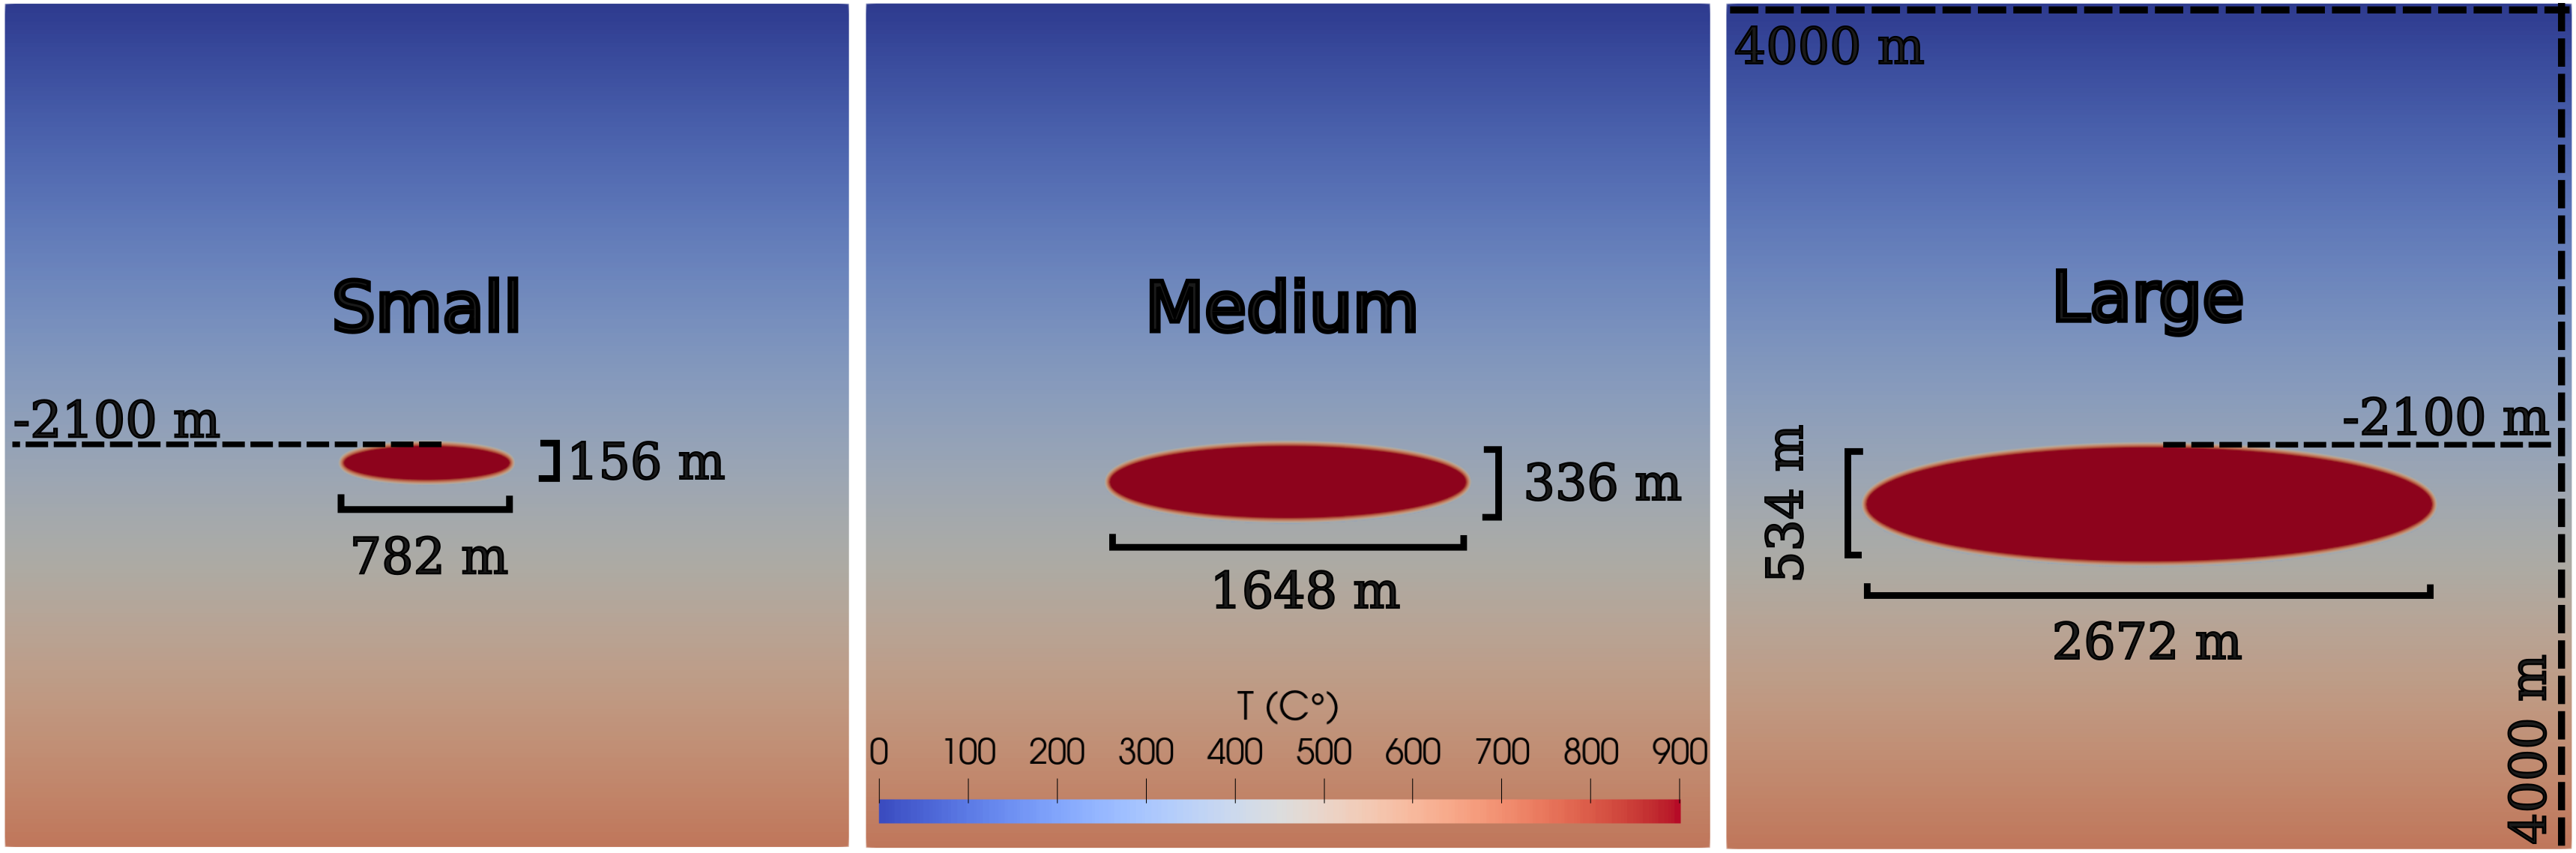
\includegraphics[width=1\linewidth]{img/chapter2/sim_setup/ic_cut.png}
    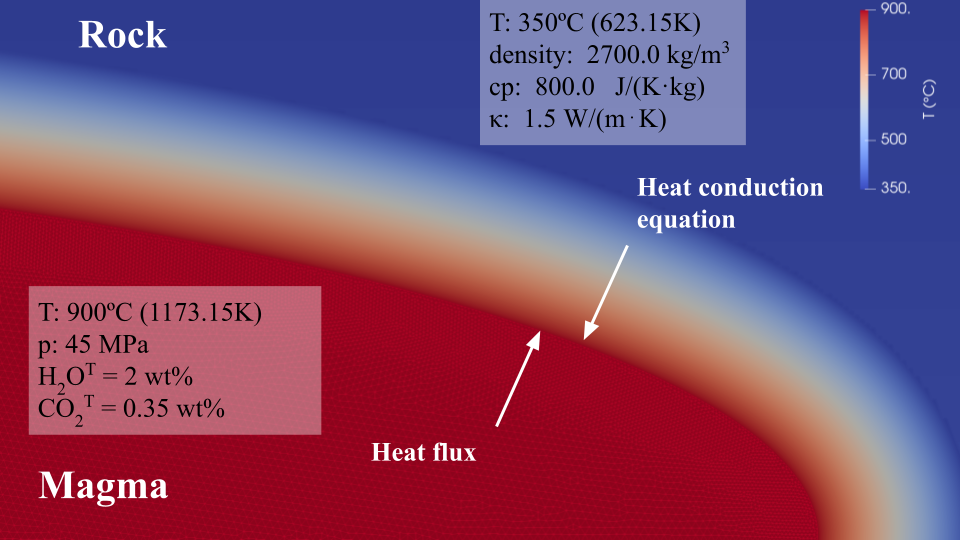
\includegraphics[width=1\linewidth]{img/chapter2/sim_setup/setup.png}
    \caption{Temperature field for the 2D convection 1c benchmark once it has reached the final steady state stage}
    \label{fig:enter-label}
\end{figure}



\chapter{Results}
%Introductions

%Typology: thermal evolu, pressure, velocity:  2D space-time distrinution. Secondary props: This is what simulations produce, and then we focus on....... whatever is the scope for us.

%One Reference simulations where everything is explained

%The others serve to see what changes and what not: effect of size, press, vols...

%Then we explain all together 

\subsubsection{Chapter overview}
In the present chapter, the results of the previously described simulations are presented. On a first instance, I discuss the information and the data that can be obtained from this type of numerical simulations, and which part of this data is of most interest for the development of the present work. Next, a full and detailed description of the results for one of the simulations, that will be considered the \textit{base} simulation is carried on. Following this description, the focus will move towards the effect of the different parameters such as size or volatile content and how these modify the evolution of the magma pocket with regard to the \textit{base} simulation. To finish, a joint and comparative analysis of the results of every simulation is presented.

\section{Typology of the results}
Numerical simulations of magma dynamics produce the 2D space-time distribution of the magmatic phases, thus, a number of solved variables at each point in space, during a given simulated time. Primary variables obtained from the simulations are pressure, velocity and temperature. These variables standalone fully describe the evolution of the magmatic system and are main source of information fo the present work, although there are other sets of variables, or rather properties that are useful to better understand the complex physics, which are considered secondary in the sense that they are not the direct solution of the flow and energy equations. These are the magma properties described in the previous chapter: density, viscosity, phases fractions, heat capacity and thermal conductivity and others. These secondary properties usually have a more direct link to real life observations, and are easier to interpret than the primary variables, which can have an abstract component to them, and are not as straightforward to translate into physically meaningful processes.

In summary, the output of the simulations can be divided into: 
\begin{enumerate} 
	\item Kinematic and dynamic flow fields, which include the 2D velocity distribution, shear ans strain fields, convective patterns and stagnant fields
	\item Temperature field evolution, which includes temperature profiles and cooling rates.
	\item Density, crystal and volatile distribution, which include both solid and gas fraction fields, latent heat effects, magma rheology evolution and possible mush/solidification zones.
	\item Thermal properties fields such as heat capacity and thermal conductivity, which include thermodynamic changes due to composition and phase change. 
\end{enumerate}

Within the scope of the present work, the most relevant variable is the temperature, since the main interest lies on the thermal evolution of the magma beneath the surface of the Krafla caldera. However, the rest of the primary variables should no be overlooked, since the relations between them are tight and of great importance. As a direct effect of the temperature (and to a lesser extent, pressure), particular attention is payed in the crystallinity fields, since they are visually more accessible in assessing the stability conditions of mushy zones or solidification fronts.

\section{Base simulation results}
In this section I present the results of the \textit{base} simulation, starting with the temperature, pressure and velocity, followed by the secondary properties. For this particular simulation, all the secondary properties are presented.

\subsubsection{Temperature}
As it has already been mentioned, the initial temperature of the magmatic system is set to 900°C, whereas the temperature of the host rock domain follows the local geothermal gradient. 
Figure \ref{fig:temperature}a shows the temperature evolution over 500 hundred years, while figure \ref{fig:temperature}b shows the integrated temperature time series over that same period of simulated time. As it can be seen, the temperature decrease during the first 60 years is quite steep, quickly going from 900°C to around 830°C, which translates into a cooling rate of 1.17 °C/year. From then on, the temperature is kept quasi constant. This is easily visible as well on the color scale, since the snapshots between 60 and 500 years seem to show the same temperature (light blue color); and more so on the integrate temperature plot, which shows an almost asymptotical behavior, with a sub-horizontal, negative slope of ~$0.004$. This slow cooling is not linear nor smooth, but instead adopts a stepped behavior, with local temperature minima followed by local maxima giving the curve its characteristic serrated shape.



\begin{figure}
	\centering
	\begin{tikzpicture}
		\node[inner sep=0pt] (img1) at (0,0) {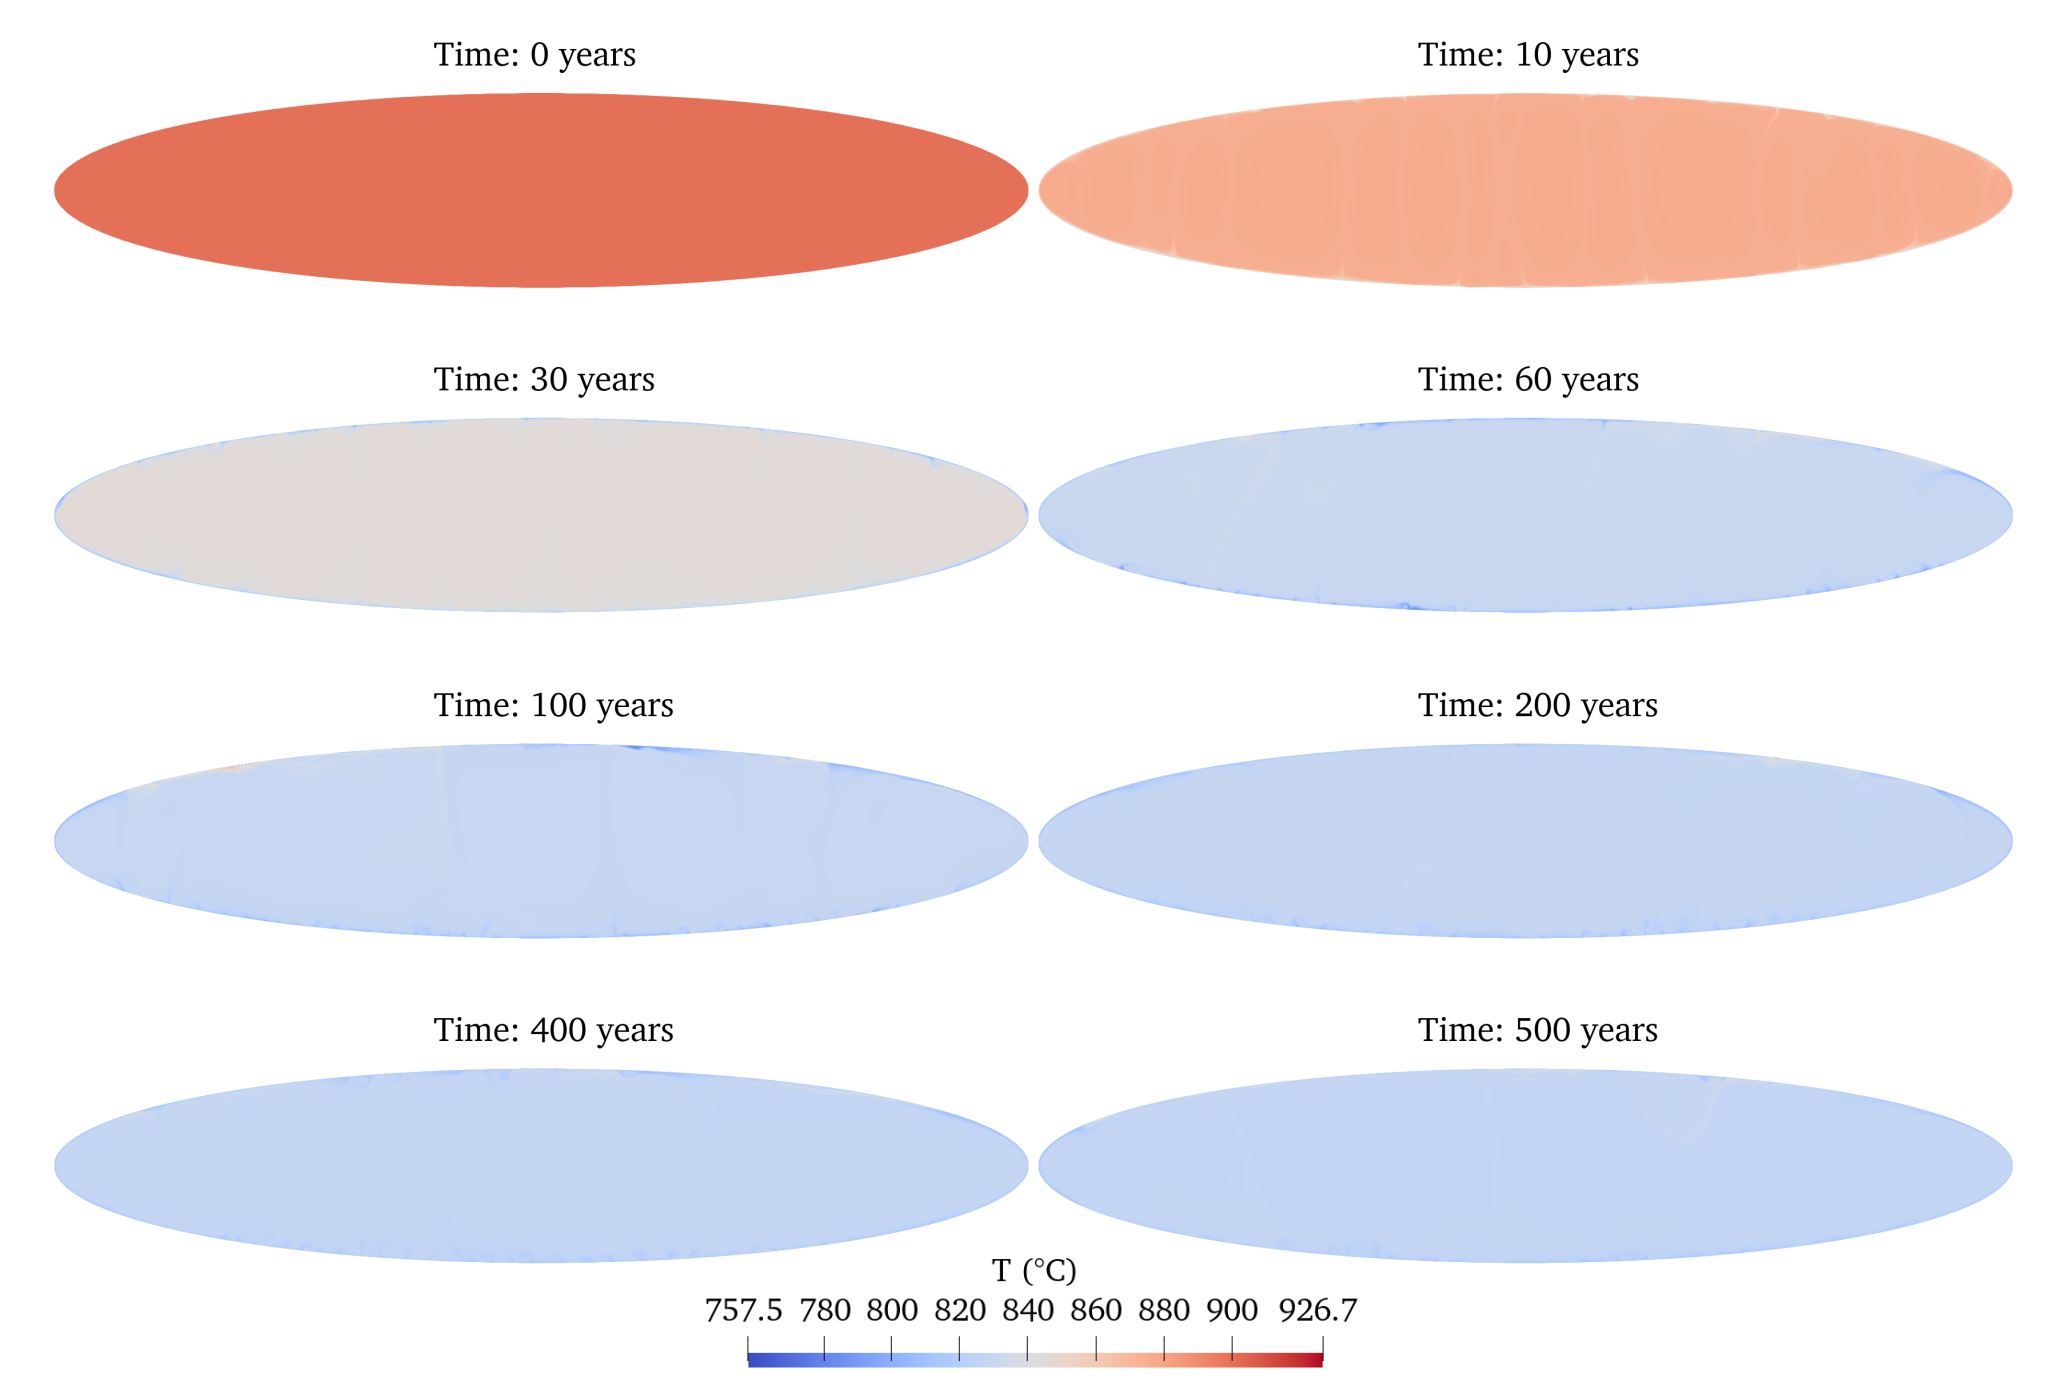
\includegraphics[width=1\linewidth]{img/chapter3/temp_2.png}};
		\node[anchor=north east, xshift=-8pt, yshift=-5pt] at (img1.north east) {\textbf{(a)}};
	\end{tikzpicture}
	\begin{tikzpicture}
		\node[inner sep=0pt] (img2) at (0,0) {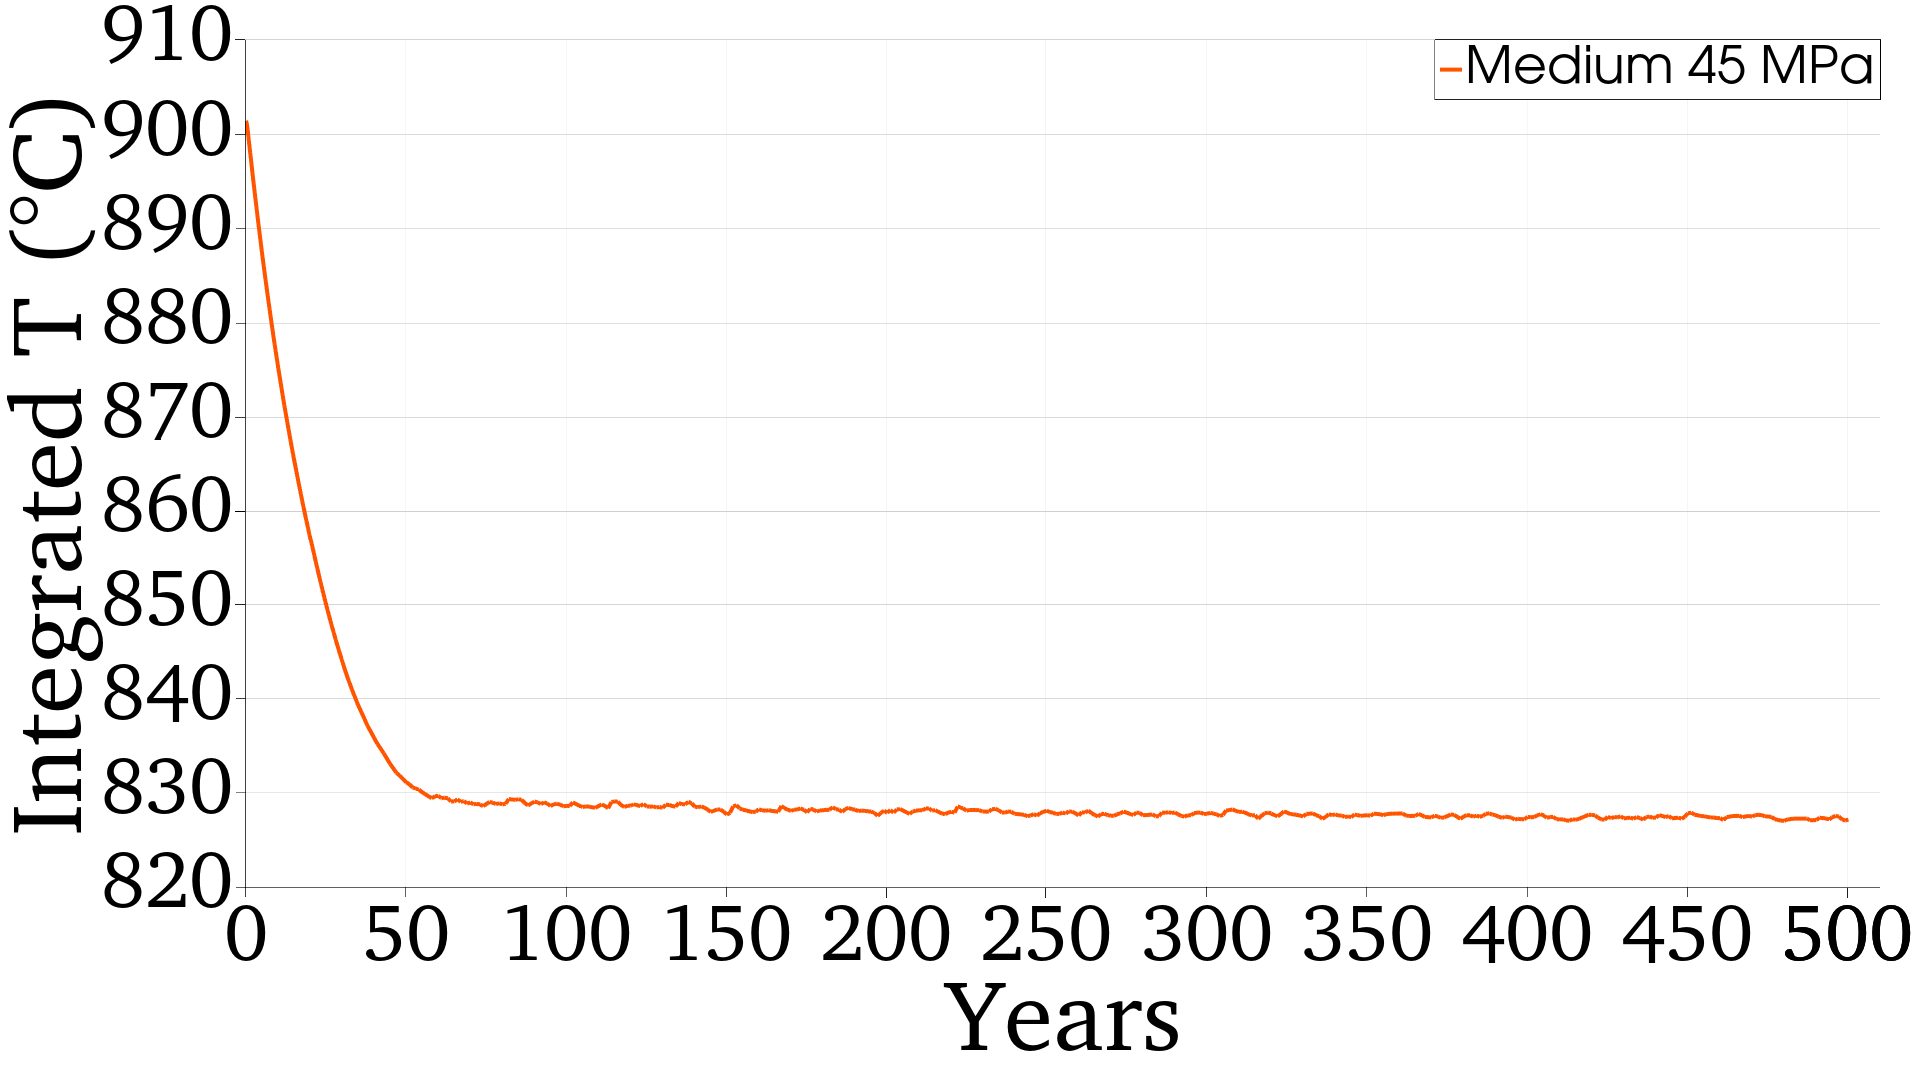
\includegraphics[width=1\linewidth]{img/chapter3/integrated_1.png}};
		\node[anchor=north east, xshift=-8pt, yshift=-5pt] at (img2.north east) {\textbf{(b)}};
	\end{tikzpicture}
	
	\caption{a) Shows snapshots of the simulations at different times up to 500 years. 
		b) Shows the integrated temperature over the whole domain}
	\label{fig:temperature}
\end{figure}

\begin{figure}
	\centering
	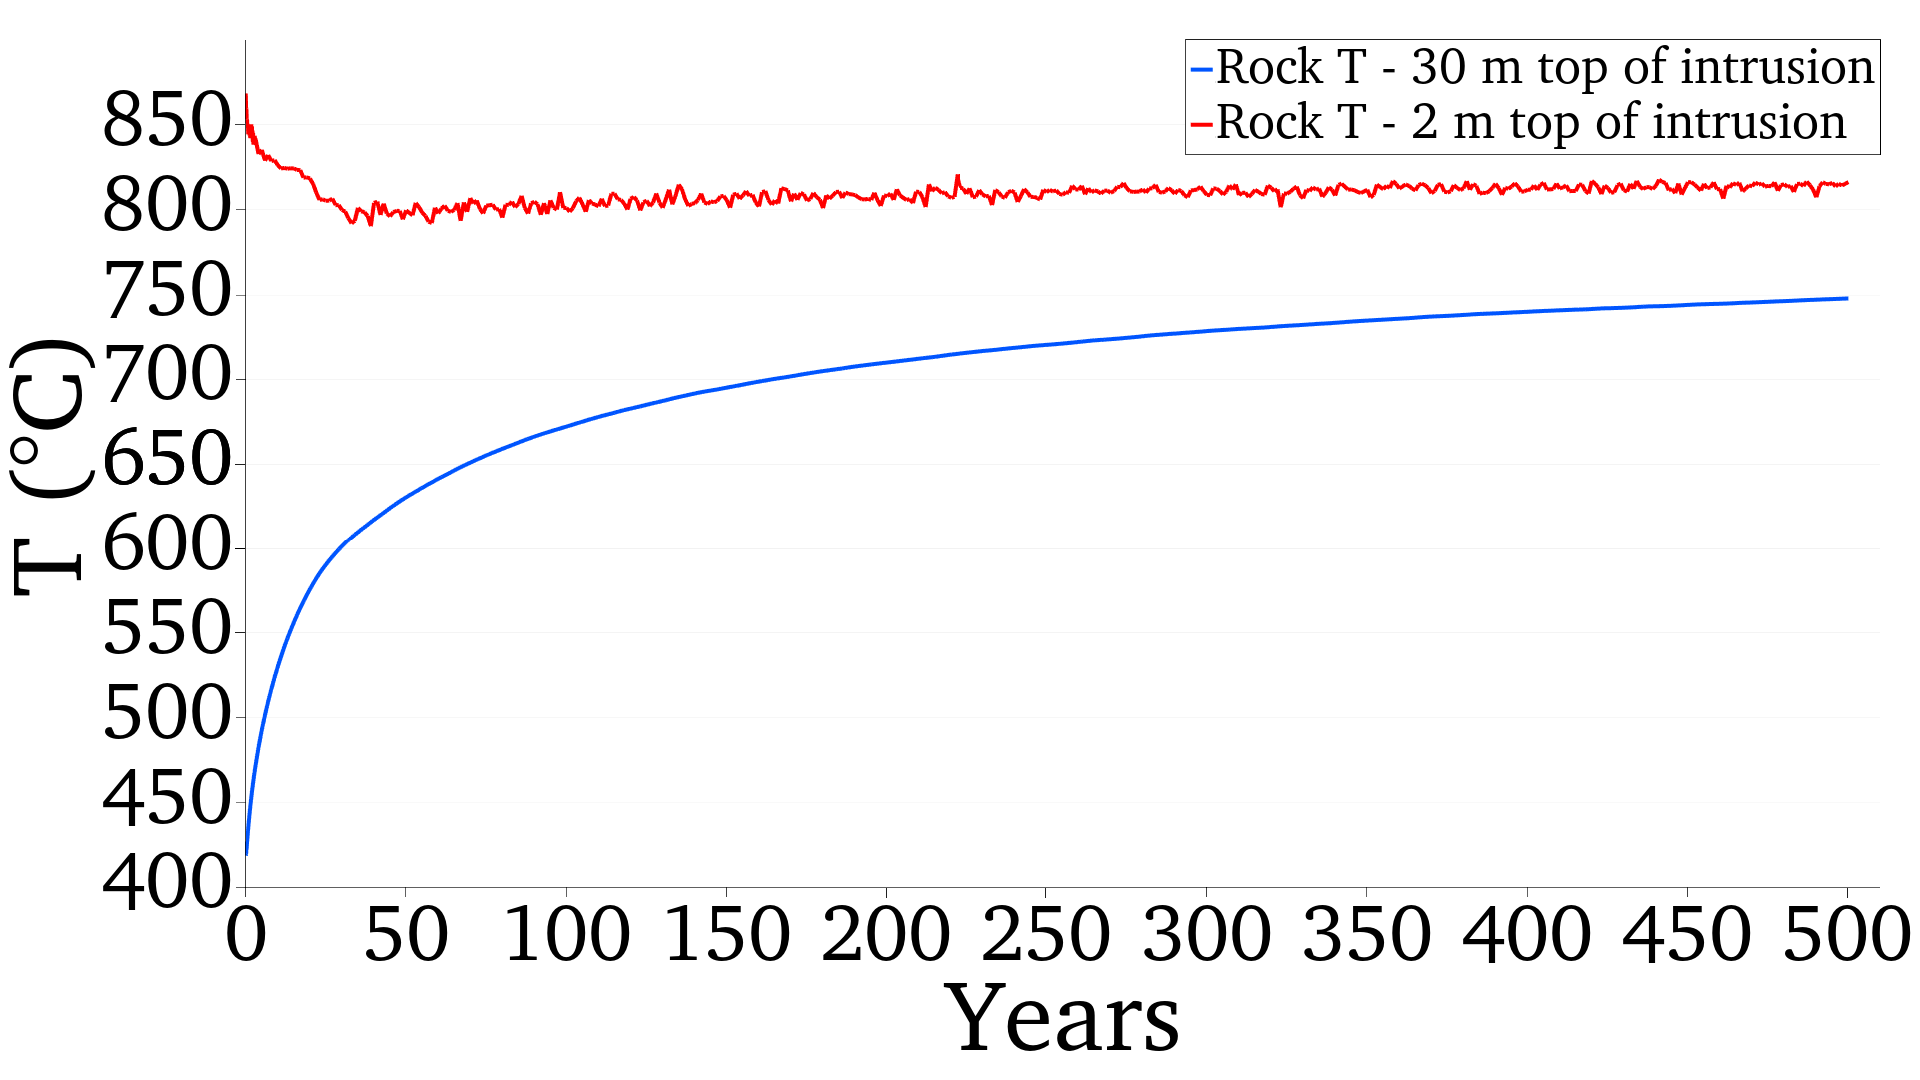
\includegraphics[width=1\linewidth]{img/chapter3/rocks_2_points.png}
	\caption{Temperature field for the 2D convection 1c benchmark once it has reached the final steady state stage}
	\label{fig:rock_2_points}
\end{figure}


\subsubsection{Velocity}
Initial velocity is set to be zero at the boundaries, for the whole duration of the simulations, and a value close to zero, $1\times10^{-8}$ m/s in this case, in order to favor numerical stability. Immediately after the first few time steps, convection begins, developing clear convective cells, easily visible in figure \ref{fig:velocity}a. The faster velocity registered during the simulation is 0.0049 m/s at the early stages of the simulation, specifically after 0.7 years (8.4 months). From this point on, the highest simulated velocities are always slower, behaving similarly as the temperature and semi-stabilizing oscillating between values of the order of  $1\times10^{-4}$ m/s and $1\times10^{-5}$ m/s. This 
As time progresses, convection slows down and evolves into less organized and defined state, exhibiting a more chaotic behavior.
\begin{figure}
	\centering
	\begin{tikzpicture}
		\node[inner sep=0pt] (img1) at (0,0) {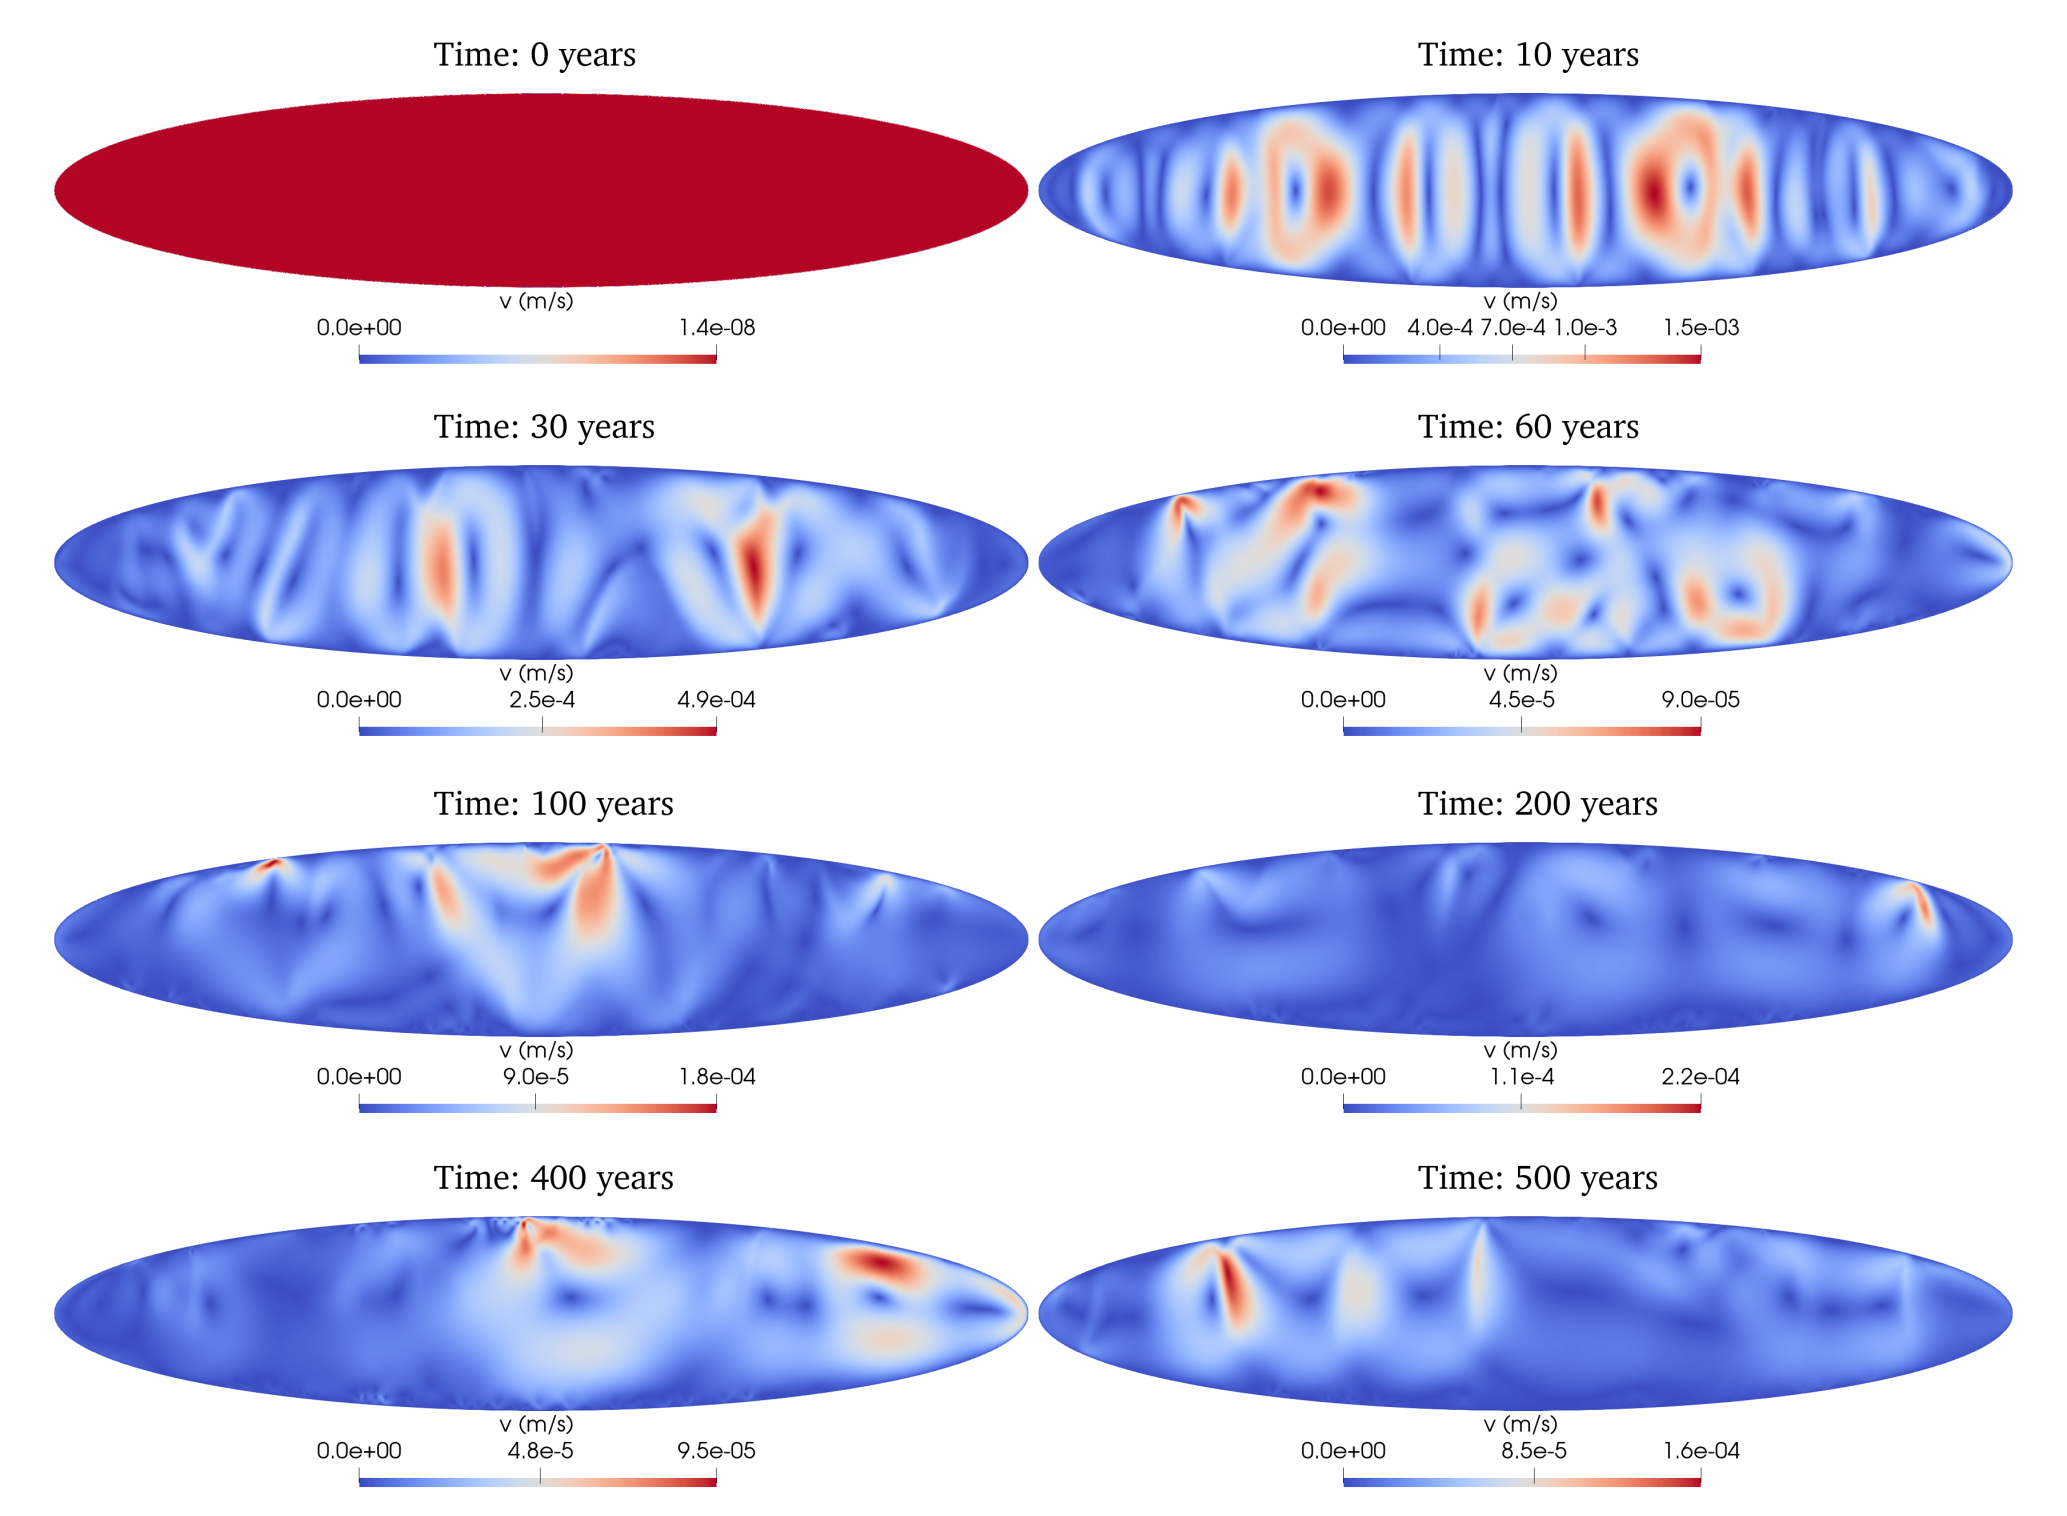
\includegraphics[width=1\linewidth]{img/chapter3/velocity/velocities.png}};
		\node[anchor=north east, xshift=-8pt, yshift=-5pt] at (img1.north east) {\textbf{(a)}};
	\end{tikzpicture}
	\begin{tikzpicture}
		\node[inner sep=0pt] (img2) at (0,0) {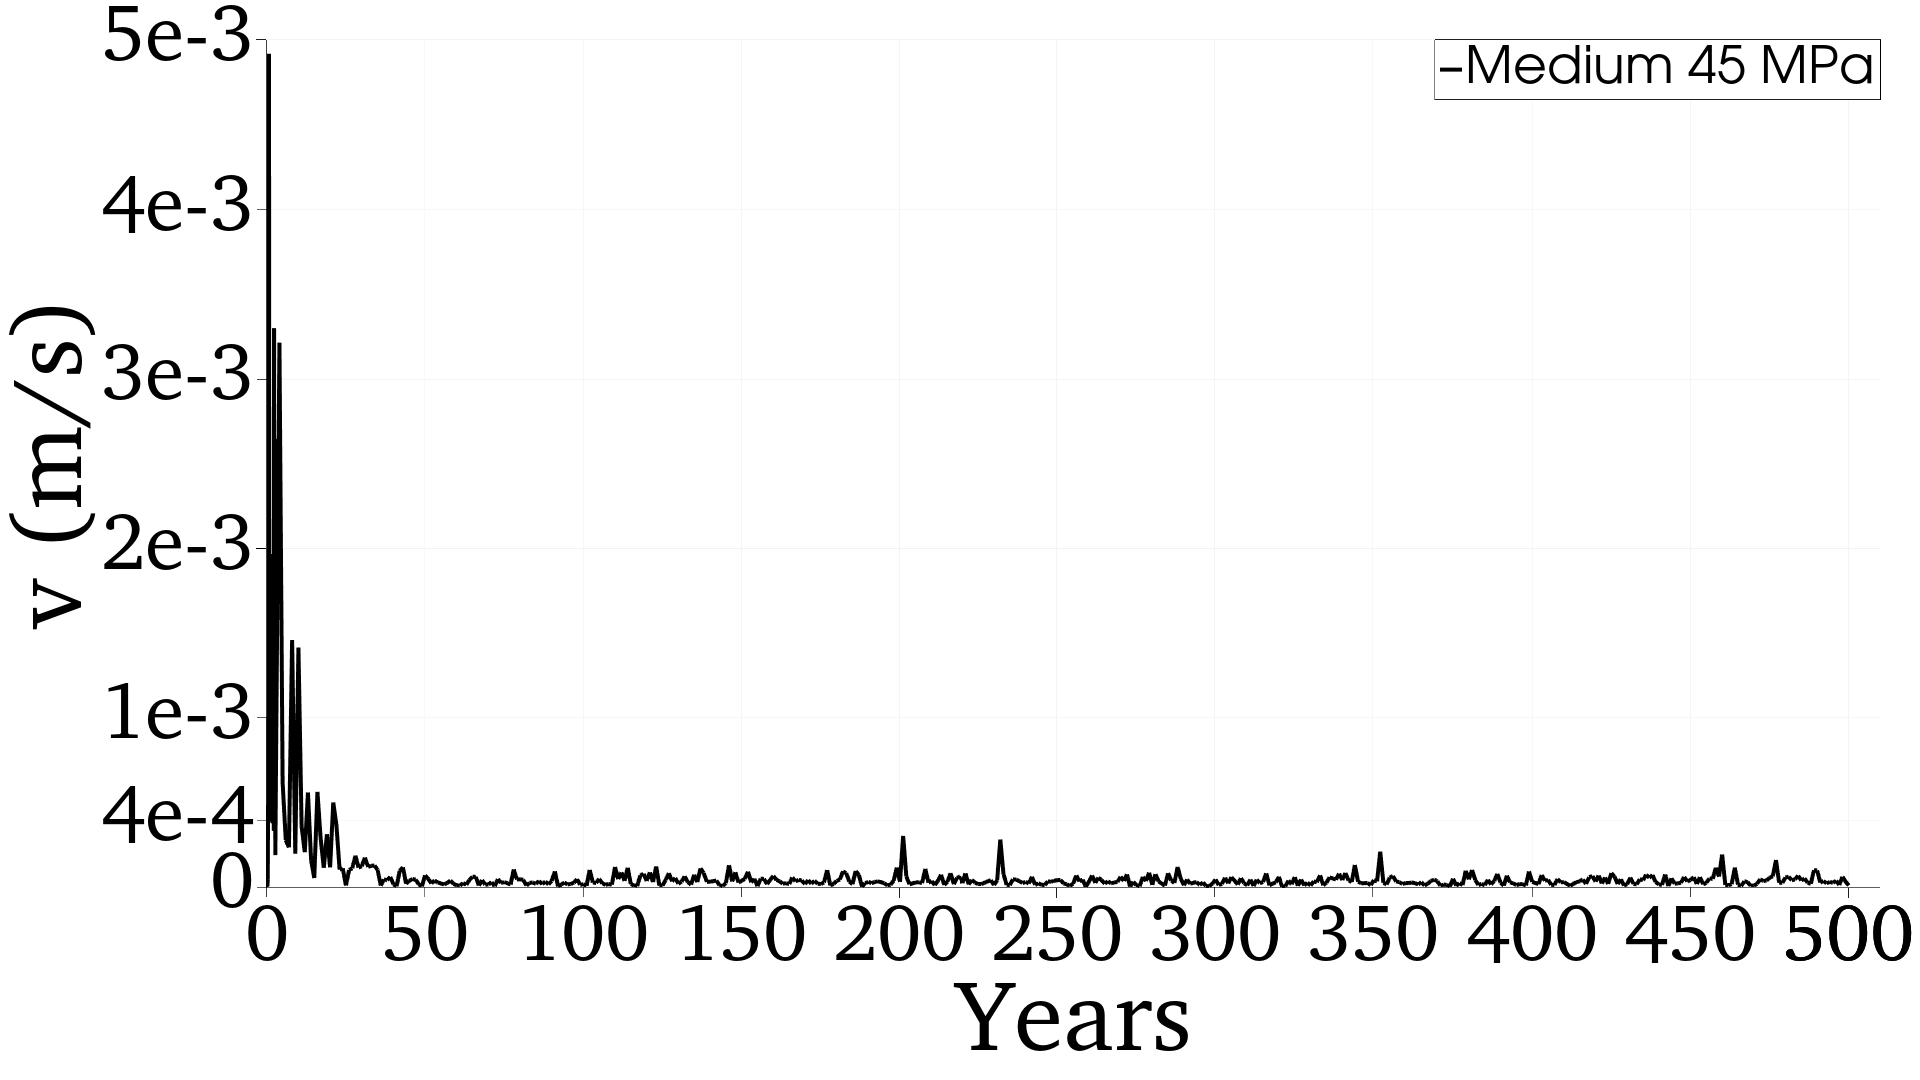
\includegraphics[width=1\linewidth]{img/chapter3/velocity/random_point.png}};
		\node[anchor=north east, xshift=-8pt, yshift=-5pt] at (img2.north east) {\textbf{(b)}};
	\end{tikzpicture}
	\caption{a) Shows snapshots of the simulations at different times up to 500 years. 
		b) Shows the integrated temperature over the whole domain}
	\label{fig:velocity}
\end{figure}


\subsubsection{Pressure}
\begin{figure}
	\centering
	\begin{tikzpicture}
		\node[inner sep=0pt] (img1) at (0,0) {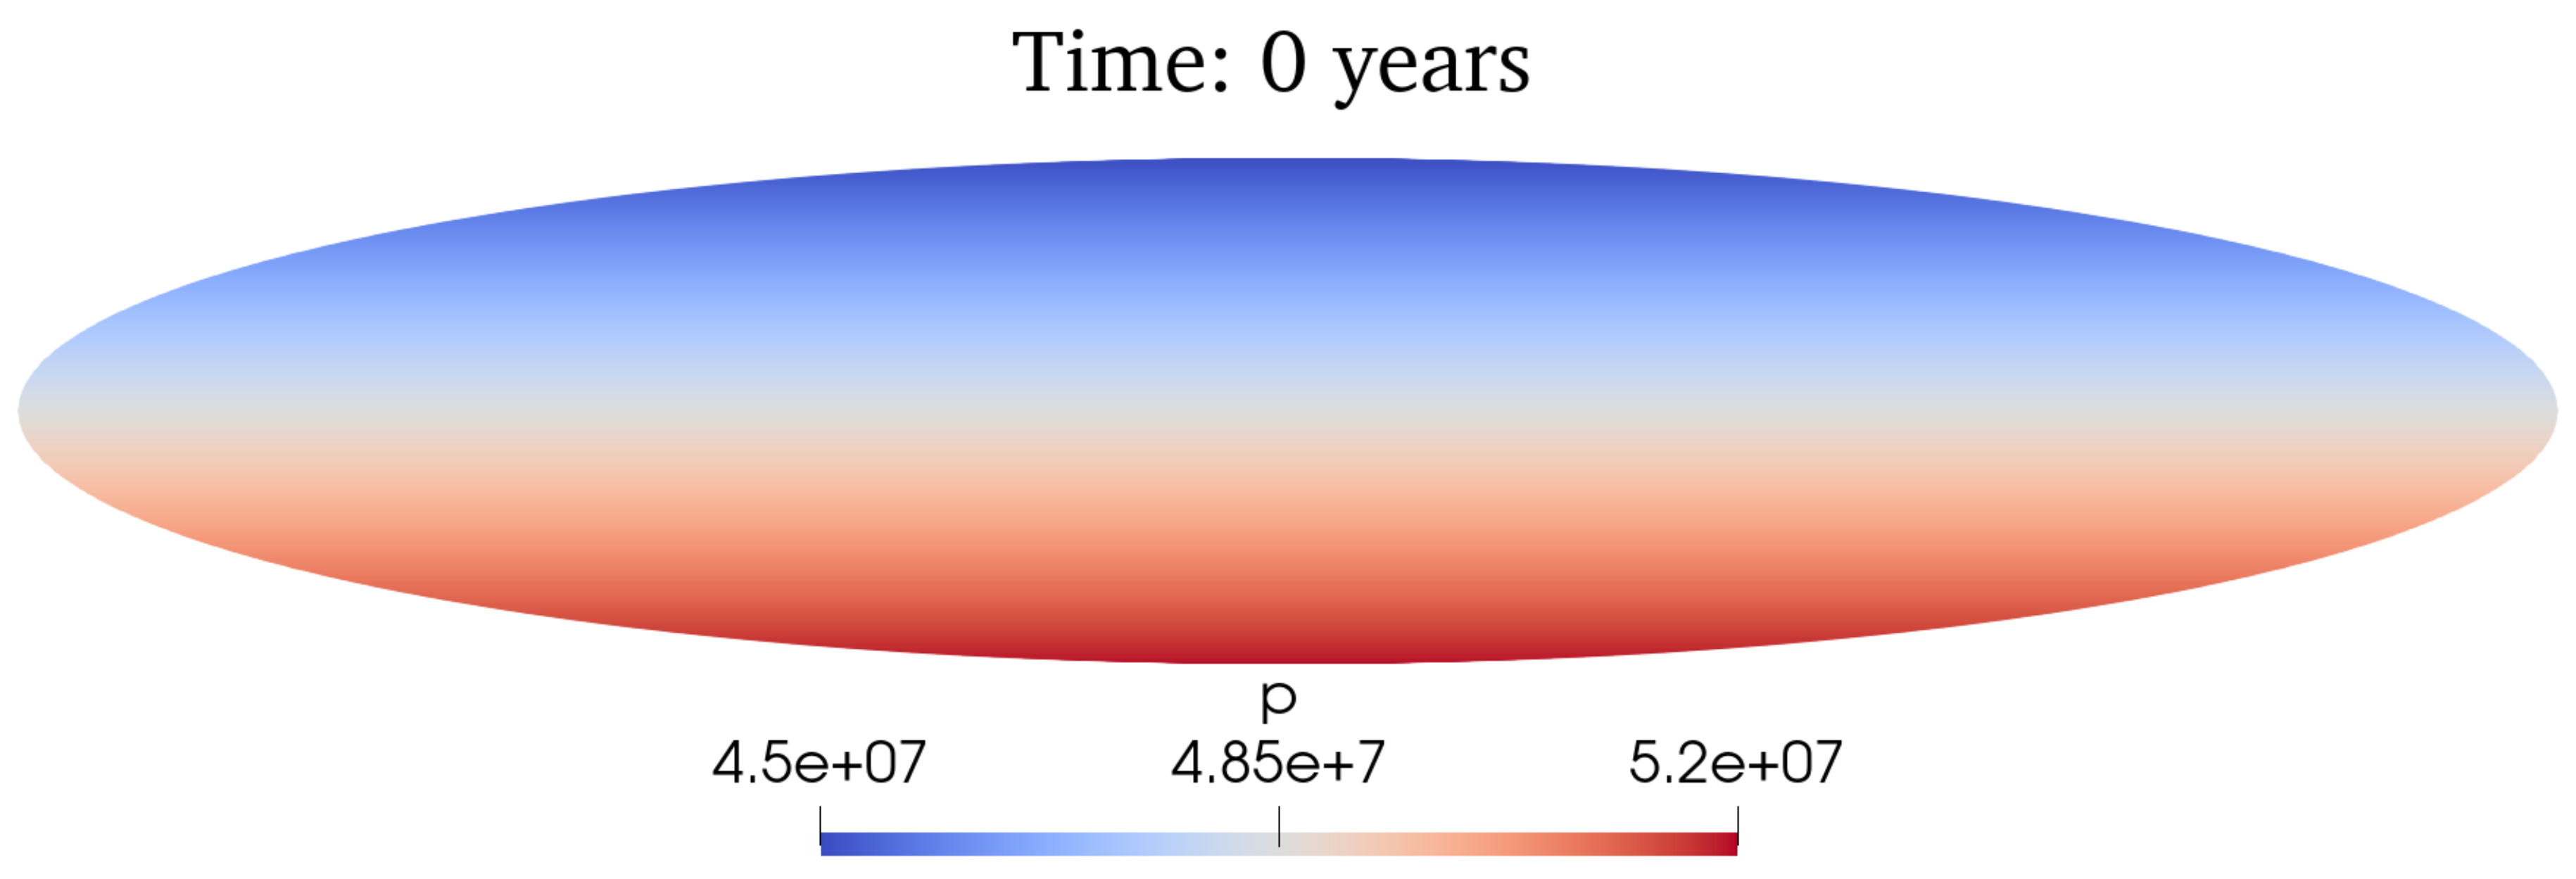
\includegraphics[width=1\linewidth]{img/chapter3/pressure/0_p.png}};
		\node[anchor=north east, xshift=-8pt, yshift=-5pt] at (img1.north east) {\textbf{(a)}};
	\end{tikzpicture}
	\begin{tikzpicture}
		\node[inner sep=0pt] (img2) at (0,0) {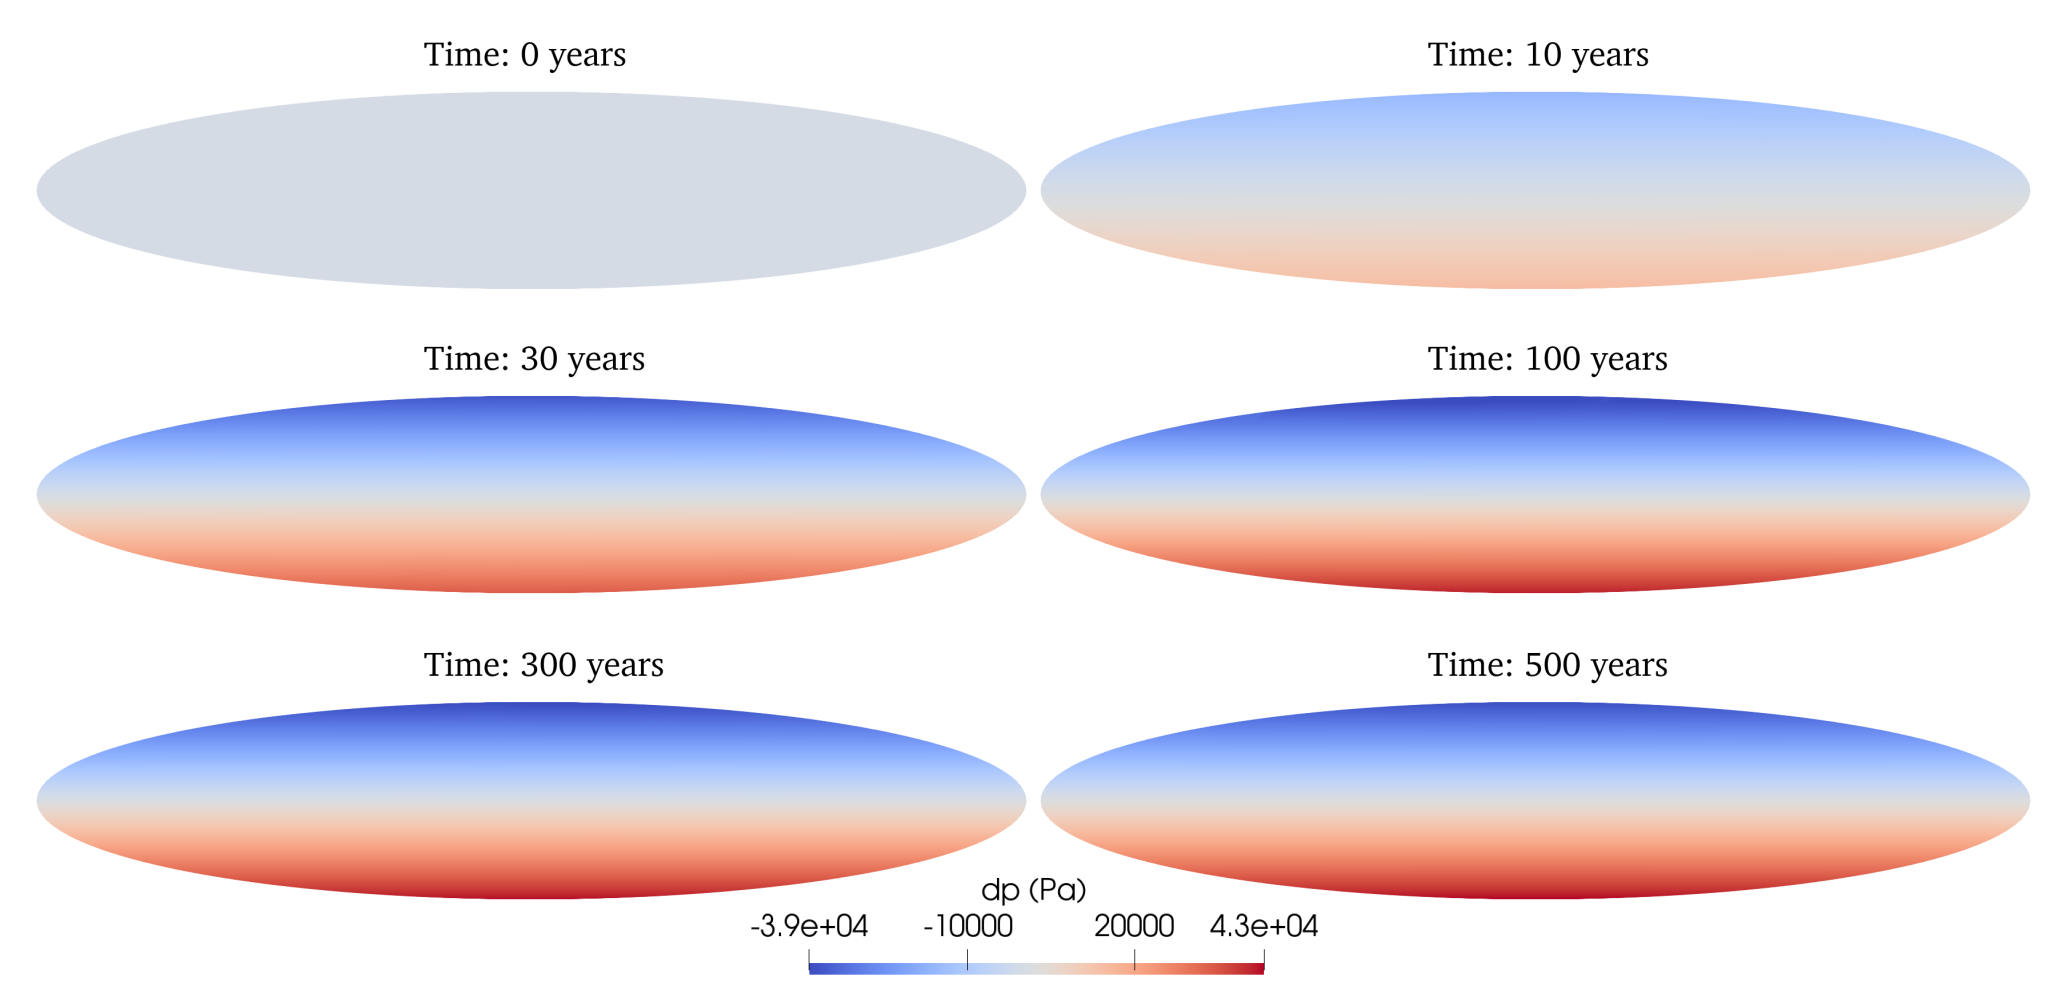
\includegraphics[width=1\linewidth]{img/chapter3/pressure/dp.png}};
		\node[anchor=north east, xshift=-8pt, yshift=-5pt] at (img2.north east) {\textbf{(b)}};
	\end{tikzpicture}
	\begin{tikzpicture}
		\node[inner sep=0pt] (img2) at (0,0) {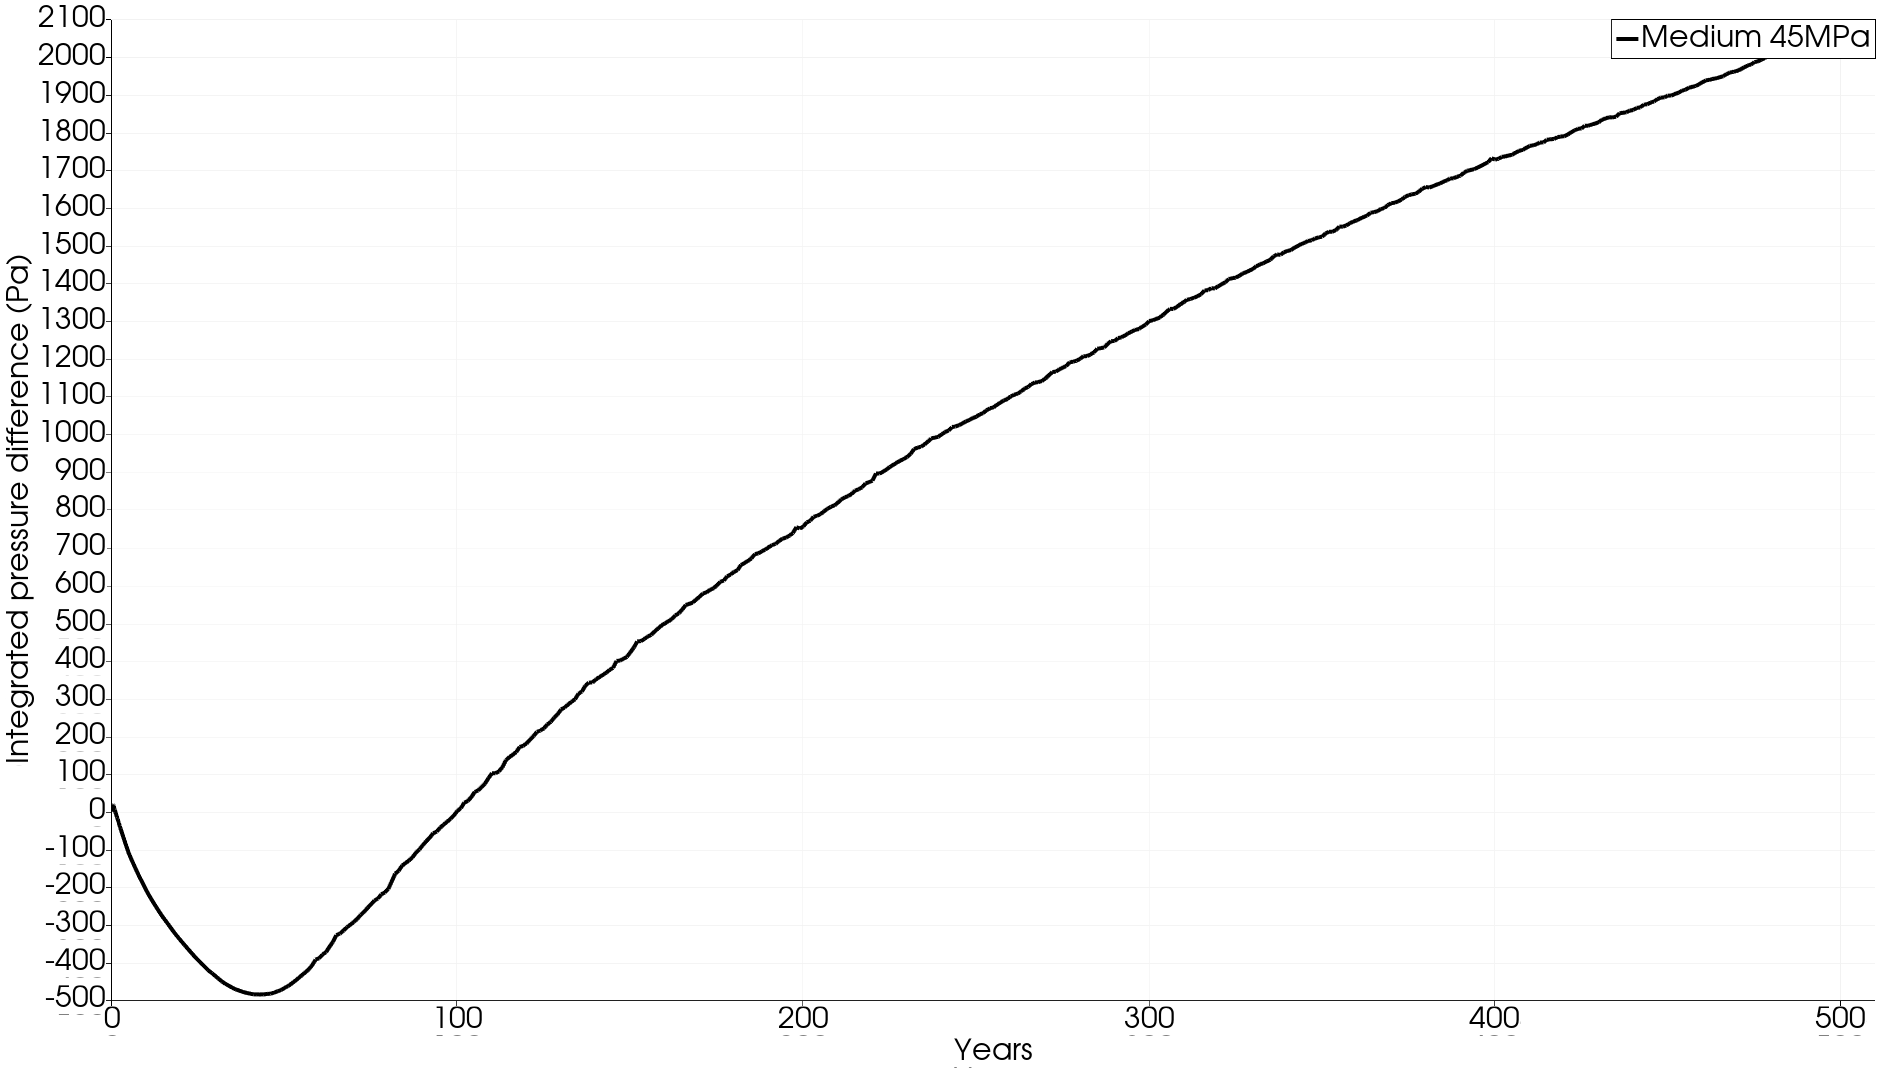
\includegraphics[width=1\linewidth]{img/chapter3/pressure/integrated_dp.png}};
		\node[anchor=north east, xshift=-8pt, yshift=-5pt] at (img2.north east) {\textbf{(c)}};
	\end{tikzpicture}
	\caption{a) Shows snapshots of the simulations at different times up to 500 years. 
		b) Shows the integrated temperature over the whole domain}
	\label{fig:pressure}
\end{figure}
% Insert further chapters using the following syntax
% \input{Source_Folder_Name/FileName}


\cleardoublepage
\phantomsection
\addcontentsline{toc}{chapter}{\bibname}
\small
\bibliographystyle{plain}
\bibliography{thesis}

\end{document}
